\documentclass[xcolor=pdftex,dvipsnames,table,notheorems]{beamer}
\usetheme{Madrid}
\usepackage{lmodern}
\setbeamercovered{dynamic}
\usepackage{wrapfig}
\setbeamertemplate{navigation symbols}{}
\usepackage[absolute,overlay]{textpos}
%\usepackage{hyperref}
\usepackage{graphics}
\usepackage[T1]{fontenc}
\usepackage{amsmath, amssymb,mathtools}
\usepackage[utf8]{inputenc}
\usepackage{hyperref}
\usepackage{bbm} 
\usepackage{graphicx}
\usepackage{appendixnumberbeamer}
\usepackage{color}
%\usepackage{xcolor}
\usepackage{subcaption}
\usepackage{centernot}
\usepackage{booktabs}
\usepackage{threeparttable}
\usepackage{tikz}
\usetikzlibrary{arrows.meta}
\usepackage{pgfplots}
\pgfplotsset{compat=1.18}
\usepackage{comment}
\setbeamercovered{invisible}
\usepackage[dvipsnames]{xcolor}
\usepackage{soul}
\usepackage{xcolor}
\usepackage{comment}

\newcommand\independent{\protect\mathpalette{\protect\independenT}{\perp}}
\def\independenT#1#2{\mathrel{\rlap{$#1#2$}\mkern2mu{#1#2}}}

\usepackage{amsthm}
\setbeamertemplate{theorems}[numbered]
\newtheorem{theorem}{Theorem}
\newtheorem{corollary}{Corollary}[theorem]
\newtheorem{lemma}{Lemma}
\newtheorem{proposition}[theorem]{Proposition}
\newtheorem{assumption}{Assumption}
\newtheorem{definition}{Definition}


\newcommand*{\boxedcolor}{red}
\makeatletter
\renewcommand{\boxed}[1]{\textcolor{\boxedcolor}{%
  \fbox{\normalcolor\m@th$\displaystyle#1$}}}
  
  \newcommand{\sym}[1]{\rlap{#1}}

\let\estinput=\input% define a new input command so that we can still flatten the document

\newcommand{\estwide}[3]{
		\vspace{.85ex}{
			\begin{tabular*}
			{\textwidth}{@{\hskip\tabcolsep\extracolsep\fill}l*{#2}{#3}}
			\toprule
			\estinput{#1}
			\bottomrule
			\addlinespace[.85ex]
			\end{tabular*}
			}
		}

\newcommand\norm[1]{\left\lVert#1\right\rVert}


\captionsetup[figtext]{justification=justified,font=footnotesize}

\newcommand{\figtext}[1]{%
% 	\vspace{-1.9ex}
\captionsetup{options=figtext}
\caption*{\hspace{6pt}\hangindent=1.5em #1}
}
\newcommand{\Figtext}[1]{%
\begin{tablenotes}[para,flushleft]
\hspace{6pt}
\hangindent=1.85em
#1
\end{tablenotes}
}
\newcommand{\Fignote}[1]{\Figtext{\emph{Note:~}~#1}}
\newcommand{\Figsource}[1]{\Figtext{\emph{Source:~}~#1}}


\usecolortheme[named=Blue]{structure}

\setbeamertemplate{caption}[numbered]{}


\newcommand\bfootnote[1]{%
  \begingroup
  \renewcommand\thefootnote{}\footnote{#1}%
  \addtocounter{footnote}{-1}%
  \endgroup
}

\definecolor{col_before}{HTML}{489c74}
\definecolor{col_after}{HTML}{cc640c}

\usepackage[dvipsnames]{xcolor}
\graphicspath{{../figures/}}
\begin{document}
\title[Reformas Ótimas da Previdência]{\large{Reformas Ótimas da Previdência:} \\ Uma Aplicação aos Dados Administrativos Brasileiros}
\author{Gustavo Gonzaga (PUC-Rio) \\ Gabriel Lemos (MIT Sloan) \\ Juan Rios (PUC-Rio)}
\date{IPEA Rio de Janeiro}
\date{\today}



\maketitle


%%%%%%%%%%%%%%%%%%%%%%%%%%%%%%%%%%%%%%%%%%%%%%%%%%%%%%%%%%%%%%%%%%%%%%%%%%%%%%%%%%%%%%%%%%%%%%%%%%%%%%%%%%%%%%%%%%%%%%%%%%%%%%%%%%%%%%%%%%%%%%%%%%%%%%%%%%%%%%%%%%%%%%%%%%%%%%%%%%
%\beamerdefaultoverlayspecification{<+->}

\begin{frame}{Gastos do Governo Federal Brasileiro}
    \centering
    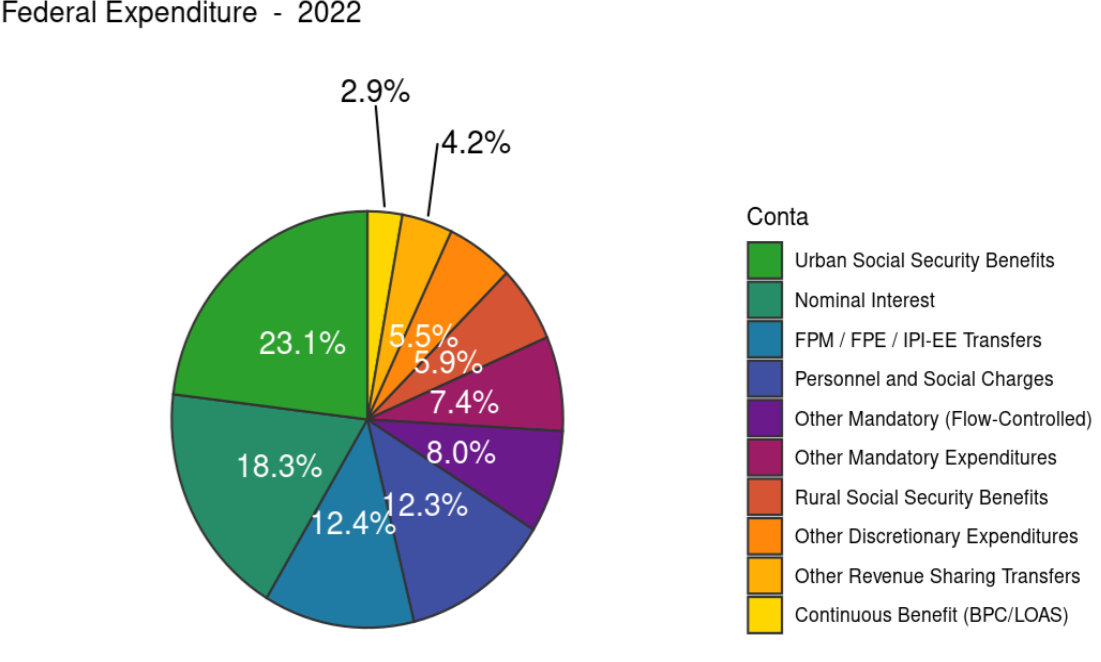
\includegraphics[width=.9\linewidth]{image37.png}
\end{frame}

\begin{frame}
\frametitle{Motivação}
    \begin{itemize}
        \item A reforma previdenciária é uma questão central em todo o mundo, mas o Brasil é um caso especialmente relevante
        \begin{itemize}
            \item O Brasil gasta muito com aposentadorias: 10.4\% do PIB em 2019 (média da OCDE: 7.7\%)
            \item Esse gasto elevado ocorre apesar de uma razão de dependência dos idosos relativamente baixa: 15.8\% em 2022 (média da OCDE: 31.3\%)
        \end{itemize}
        \item Houve tentativas recentes de conduzir análises de bem-estar dessas reformas previdenciárias usando fórmulas de estatísticas suficientes
        \item O desenho ótimo foi estudado na literatura estrutural e teórica
    \end{itemize}
\end{frame}

\begin{frame}
\frametitle{Contexto e Pergunta de Pesquisa}
    \begin{columns}
        \begin{column}{0.55\textwidth}
            \begin{itemize}
                \item Exploramos uma reforma da regra brasileira de aposentadoria por tempo de contribuição
                \begin{itemize}
                     \item Os benefícios dependem de pontos = idade + anos de contribuição
                    \item[] 
                    %\item No minimum claiming age
                    \uncover<2->{\item A reforma alterou tanto o \textbf{nível do benefício $b_L$} quanto a \textbf{inclinação do benefício $b_S$} após um limiar de pontos} 
                \end{itemize}
            \end{itemize}
        \end{column}
        \begin{column}{0.4\textwidth}
          \centering
          %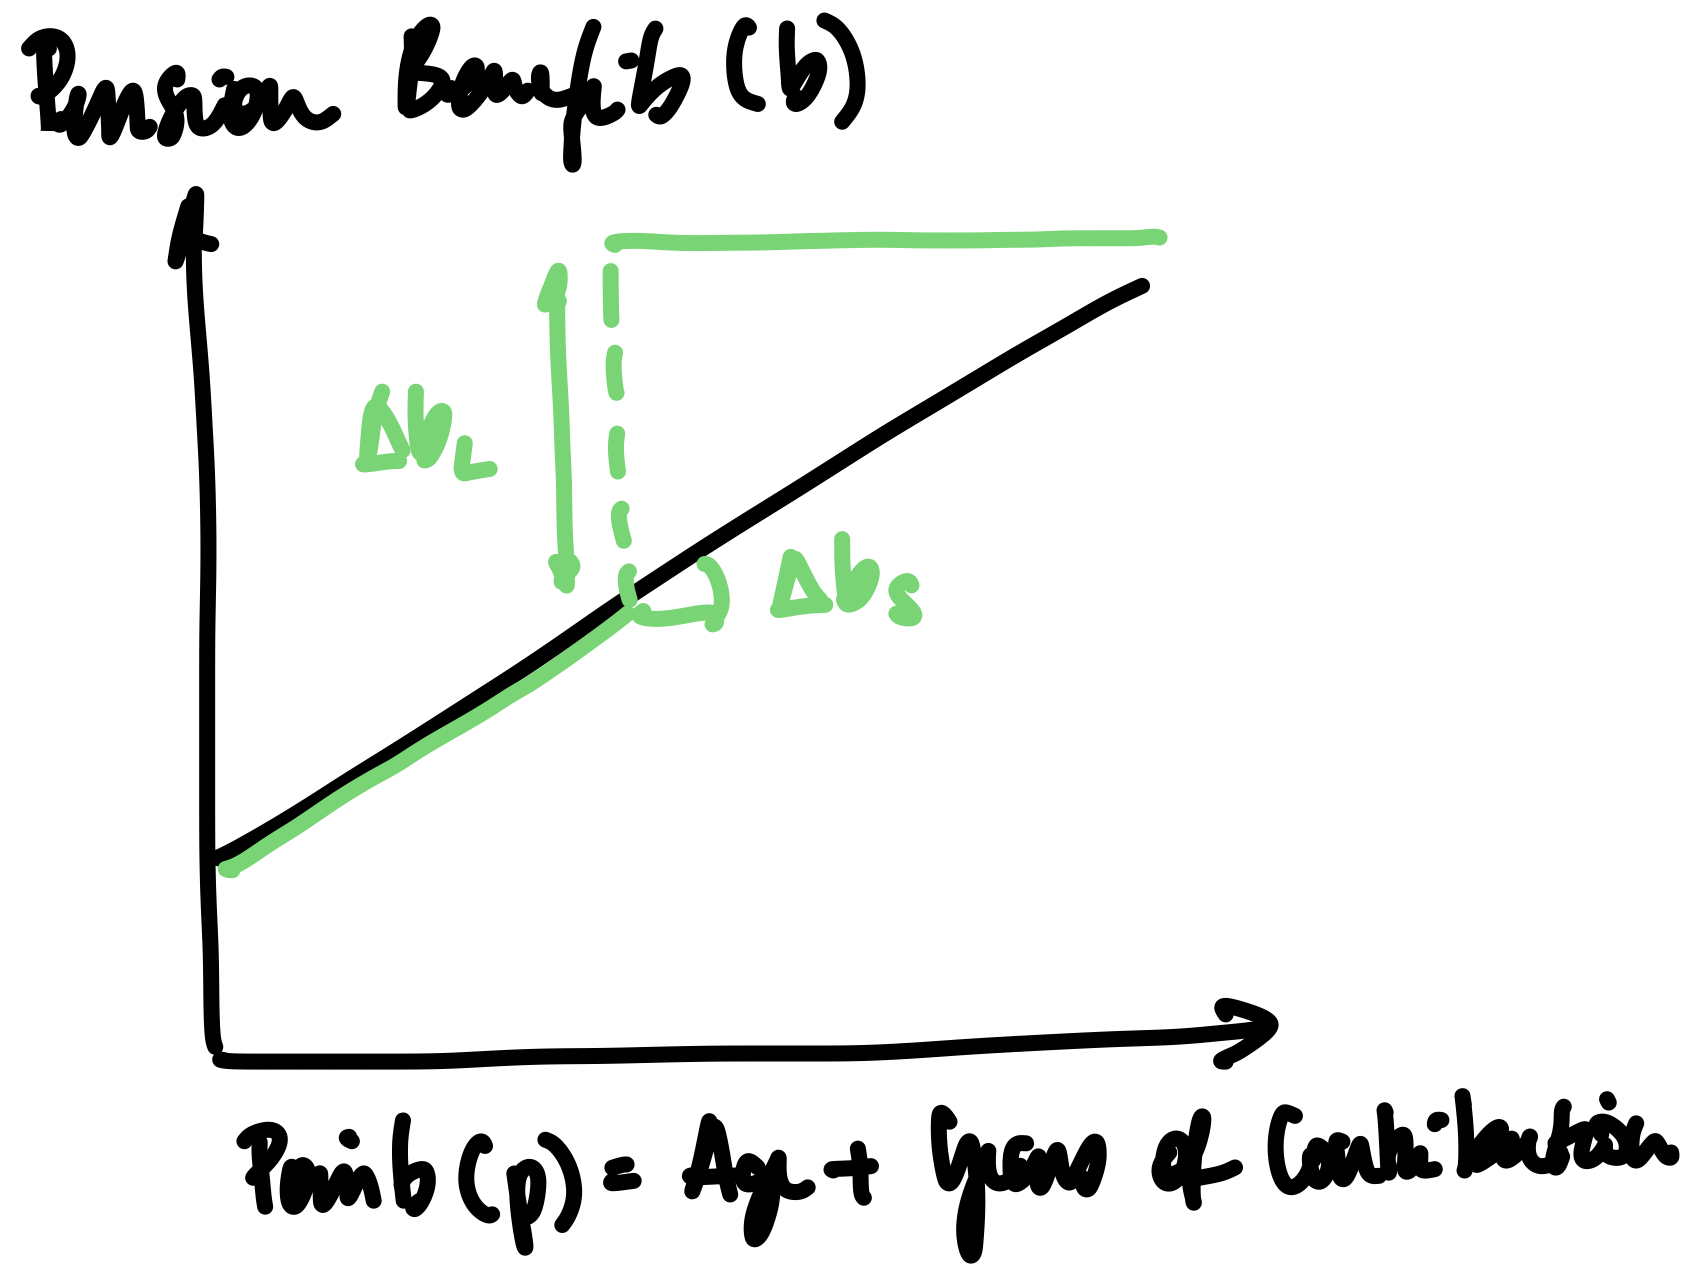
\includegraphics[width=\linewidth]{scheduleReform.png}
          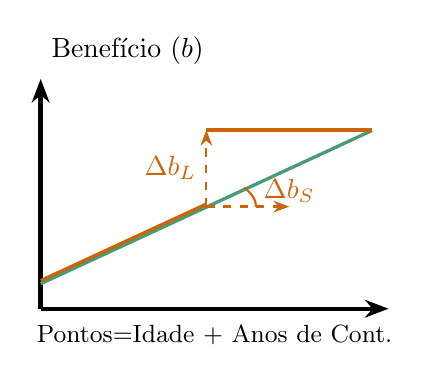
\begin{tikzpicture}
  \begin{axis}[
    width=6cm, height=4.5cm,
    axis lines=left,
    axis line style={-{Stealth[length=3mm]}, ultra thick},
    xmin=0, xmax=4.2, ymin=0, ymax=9,
    xtick=\empty, ytick=\empty, clip=false,
    xlabel={},
    xlabel style={at={(axis description cs:1.02,0)}, anchor=west},
    ylabel={},
  ]

    % Axis labels
    \node[anchor=south, rotate=0] at (axis description cs:0.25,1.02) {Benefício ($b$)};
    \node[anchor=south, rotate=0] at (axis description cs:0.5,-0.2) {\small Pontos=Idade + Anos de Cont.};

    % Black baseline line
    \addplot[very thick,col_before,domain=0:4] {0.98+1.5*x};

    % Orange shifted line (parallel, upward shift)
    \only<2->{\addplot[very thick,col_after,domain=0:2] {1.1+1.5*x};

    % Orange horizontal line
    \addplot[very thick,col_after,domain=2:4] {7};}

    % Pick a reference point along the black line
    \coordinate (A) at (axis cs:2,{1+1.5*2});
    \coordinate (B) at (axis cs:2,7); % same x, higher y (on green line)
    \coordinate (C) at (axis cs:3,{1+1.5*2}); % shift right to hit green line

     % Dashed arrows showing Δb_ℓ (vertical) and Δb_s (horizontal)
    \only<2->{\draw[col_after, dashed, thick, -{Stealth[length=2mm]}] (A) -- (B) node[midway,left] {$\Delta b_L$};
    \draw[col_after, dashed, thick, -{Stealth[length=2mm]}] (A) -- (C);
    \node[col_after] at (axis cs:3,4.6) {$\Delta b_S$};

    % Arc to show angle
  \draw[thick,col_after] (2.6,4) arc[start angle=0,end angle=22,radius=2];}

  \end{axis}
\end{tikzpicture}
          % Optionally, a caption
          % {\small Caption here}
        \end{column}
    \end{columns}
    \vspace{0.6em}
    \uncover<3>{\begin{enumerate}
        \item Qual foi o efeito de bem-estar da reforma? 
        \item Como devemos reformar essa regra?
        \begin{itemize}
            \item Precisamos separar os efeitos de bem-estar de $\Delta b_L$ e $\Delta b_S$
        \end{itemize}
    \end{enumerate}}
\end{frame}

\begin{frame}[label=mainResults]{Principais Resultados}
\begin{itemize}
    \item Qual foi o efeito de bem-estar da reforma?
    \begin{itemize}
        \item $MVPF=DAP/Custo$ mede a disposição a pagar dos beneficiários para cada R\$1 gasto na reforma (Hendren and Sprung-Keyser, 2020)
        \item Seja $\eta$ o peso médio de bem-estar atribuído aos beneficiários da reforma
        \item $WMVPF = \eta MVPF$ é o efeito de bem-estar para cada R\$1 gasto
        \item Encontramos que $MVPF \approx 0.31$ e $WMVPF\approx 0.26$
    \end{itemize}
    %\item What is the optimal local reform? How should we change $b_L$ and $b_S$ to maximize welfare increase in a budget neutral reform?
    % \item Bergstrom, Dodds and Rios (2026) mostram que a reforma ótima (que maximiza bem-estar) deve gastar em políticas com maior WPIC e arrecadar em políticas com menor WPIC
    % \begin{itemize}
    %     %\item Policymaker should spend on (raise revenue from) policies with highest (lowest) WMVPFs (Bergstrom, Dodds and Rios, 2026)
    %     \item No caso neutro em orçamento, $WPIC = WMVPF \Rightarrow$ aumentar a inclinação do benefício e reduzir o nível do benefício
    %     %\item (Preliminary) Optimal reform consists of increasing benefit slope and decreasing benefit level
    %     \item No caso de gasto financiado pela folha, $WPIC = WNSBD \Rightarrow$ aumentar a inclinação do benefício e financiar isso com imposto sobre a folha
    % \end{itemize}
\end{itemize}
\bfootnote{\hyperlink{literature}{\beamerbutton{literatura}}}
\end{frame}

\begin{frame}{Roteiro}
  \tableofcontents
\end{frame}

\section{Contexto Institucional e Dados}

\begin{frame}{Aposentadorias no Brasil}
    \begin{itemize}
        \item Maior programa da seguridade social no Brasil
        \begin{itemize}
            \item \alt<2->{\textbf{RGPS}}{RGPS}: trabalhadores do setor privado (90.5\% dos gastos)
            \item RPPS: servidores públicos (9.5\%)
        \end{itemize}
        \item  RGPS se divide em trabalhadores \alt<3->{\textbf{urbanos}}{urbanos} (69.2\%) e rurais (30.8\%)
        \item Trabalhadores urbanos podiam requerer segundo dois critérios:
        \begin{itemize}
            \item Idade: 60 para mulheres e 65 para homens
            \item \alt<4->{\textbf{Tempo de contribuição}}{Tempo de contribuição}: mulheres (homens) podiam requerer antes se tivessem contribuído por 30 (35) anos
        \end{itemize}
        \item 55.2\% desses trabalhadores urbanos se aposentavam por tempo de contribuição
    \end{itemize}
\end{frame}

\begin{frame}{Regra da Aposentadoria por Tempo de Contribuição}
    \begin{itemize}
        \item Aposentadoria integral equivalente a 80\% dos maiores salários desde julho de 1994 ajustados pela inflação (salário de contribuição)
        \item Benefícios limitados por um piso (salário mínimo) e um teto (5.6 salários mínimos $\approx$ percentil 90 da distribuição de renda)
        \item O fator previdenciário (benefício/salário de cont.) é função da idade, anos de cont. e expectativa de sobrevida no requerimento
        % \begin{itemize}
        %     \item May be above 1
        % \end{itemize}
        \item Os trabalhadores podem requerer e continuar no setor formal sem suspensão do benefício
    \end{itemize}
\end{frame}

\begin{frame}{Dados}
    \begin{itemize}
        \item Análise principal: dados administrativos da seguridade social (SUIBE)
        \begin{itemize}
            \item Universo dos requerimentos de aposentadoria precoce de empregados formais do setor privado entre 2012 e 2019 (2.7 M)
            \item Inclui valor do benefício, data do requerimento, fator previdenciário, anos de contribuição, data de nascimento etc.
        \end{itemize}
        \item Complementamos com
        \begin{itemize}
            \item RAIS: mede (i) histórico de contribuição antes e depois do requerimento e (ii) pagamentos na folha e imposto de renda
            \item ELSI e POF: medidas de consumo para beneficiários (idosos) e para a população em geral, necessárias para a análise de bem-estar
        \end{itemize}
    \end{itemize}
\end{frame}

\begin{frame}[label=reform]{A Reforma de 2015}
    \begin{columns}
        \begin{column}{0.48\textwidth}
            \begin{itemize}
                \item Desde 1999, os benefícios aumentavam quase linearmente com pontos (idade+anos de contribuição) 
                \item Em abril de 2015, o Congresso iniciou a discussão sobre a reforma
                \item Em junho de 2015, a reforma alterou dois parâmetros:
            \end{itemize}
        \end{column}
        \begin{column}{0.48\textwidth}
          \centering
          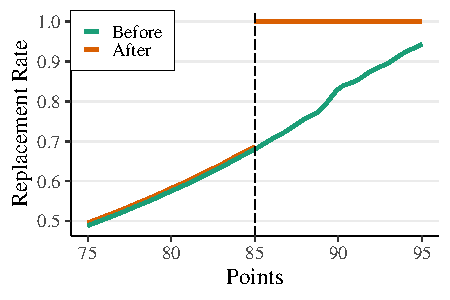
\includegraphics[width=\linewidth]{schedule_women_new.pdf}
        \end{column}
    \end{columns}
    % We first calculate the average replacement rate for each cohort in the data according to their mean input (years of contribution, wage, life expectancy etc)
    % We then take the average across cohorts 
    % The bump comes from adjustments in life expectancy.
    \begin{enumerate}
        \item o nível do benefício $b_L$ aumentou em 85 (95) pontos para mulheres (homens)
        \item a inclinação do benefício $b_S$ foi removida após o mesmo limiar de 85/95 pontos para mulheres/homens
    \end{enumerate}
    \bfootnote{\hyperlink{dataReplacement}{\beamerbutton{Dados}}
    \hyperlink{men}{\beamerbutton{Homens}}}
\end{frame}

\begin{frame}[label=rfEvidence]{Densidade de Requerimento (Dados Brutos)}
    \centering
    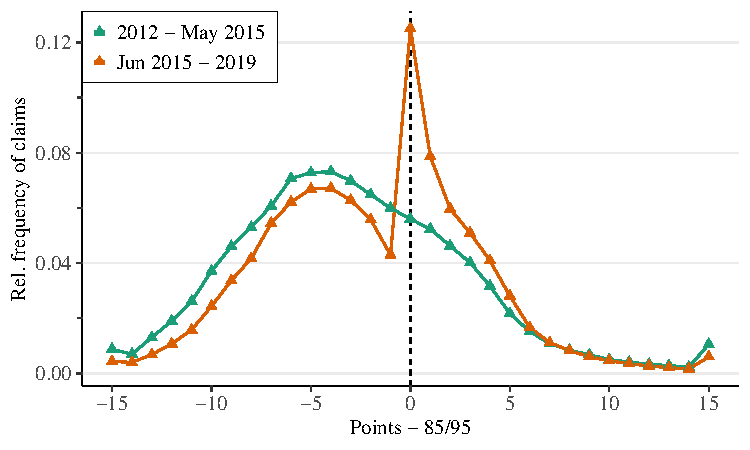
\includegraphics[width=.9\linewidth]{E3_claiming_density.pdf}
\bfootnote{\hyperlink{rfEvidenceWomen}{\beamerbutton{Mulheres}} \hyperlink{rfEvidenceMen}{\beamerbutton{Homens}}}
\end{frame}

\section{Modelo}

\begin{frame}[label=model]
\frametitle{Problema do agente}
\begin{itemize}
    \item Os agentes maximizam a utilidade esperada sujeita a uma restrição orçamentária
    \begin{align*}
        \max_{x_{it}} &\Bigg\{\sum_{s=t}^{T_i}\beta^s E[ u(x_{is})]\quad \text{ s.t. } \\
         &\quad a_{i,t+1} =(1+r)[a_{it}+y_{it}(x_{it})-\tau(x_{it})+b(x_{it})-c_{it}]\Bigg\}
    \end{align*}
    \item O vetor de escolhas $x_{it}$ inclui ativos $a_{it}$, consumo $c_{it}$, decisão de requerer benefícios, trabalho formal e informal, esforço etc.
    \item Eles carregam para o período seguinte toda a renda $y_{it}$, os ativos $a_{it}$ e os benefícios $b$ que não são usados para pagar impostos $\tau$ ou consumo $c_{it}$
    % b(x_it) should actually be b_t({x_is}s=0^t) but we are saving notation. 
\end{itemize}
\end{frame}

\begin{frame}
\frametitle{Bem-estar e orçamento do governo}
\begin{itemize}
    \item No período da reforma $t=0$, o bem-estar é $\sum_{i} \sum_{t=0}^T\beta^t E[ u(x_{it})]$
    % Juan: quero revisar esta expressão. Como cada individuo vive ate T_i, pode ser que a soma correta precise explicitar o horizonte individual, por exemplo \sum_i \sum_{t=0}^{T_i}.
    % Opinião do Codex: eu interpretaria que a forma com T_i faz mais sentido se x_{it} estiver definido apenas enquanto o individuo vive. Manter T comum so funciona se, para t>T_i, consumo, beneficio e utilidade forem definidos como zero ou se T for apenas um atalho notacional para um horizonte maximo comum.
    \item A restrição orçamentária do governo é
    \begin{align*}
        \sum_{t=0}^T \sum_i \frac{E[\tau(x_{it})]-E[b(x_{it})]}{(1+r)^t}\geq\bar G_0,
    \end{align*}
    % This is weaker than requiring that the budget closes under each state of the world. 
    \item Dois conceitos de regra de benefícios
    % technically, it also depends on states, but we are saving notation
    % Note that the actual schedule differs for those who claimed above the threshold depending on whether they claim before or after the reform
    % The counterfactual schedule is the same
    \begin{itemize}
        \item $b^c(\cdot)$: benefício contrafactual na ausência da reforma
        \item $b^a(\cdot)$: benefício observado com a reforma
    \end{itemize}
    \item Isso leva a dois conceitos distintos de vetor de escolhas
    \begin{itemize}
        \item $x^c_{it}$: sob o benefício contrafactual
        \item $x_{it}^a$: sob o benefício observado (reformado)
    \end{itemize}
    %\item These choices also may affect the state distribution
\end{itemize}
\end{frame}

\begin{frame}{Análise de Bem-Estar}
    \begin{itemize}
        \item Pelo teorema do envelope, o efeito de bem-estar por real gasto na reforma de $b^c$ para $b^a$ é:
        \begin{align*}
            WMVPF(b^c,b^a)=\frac{\sum_t \sum_i E(SMU_{it}[b^a(x^c_{it})-b^c(x^c_{it})])}{C(b^c,b^a)}
        \end{align*}
        % b_a'=b^a(x_{it}|a(x_{it})=a)
        % b_a=b(x_{it}|a(x_{it})=a)
        \item Onde $SMU_{it} \equiv \beta^t \frac{\partial u(x_{it})}{\partial c_{it}}$ é a utilidade marginal social do consumo do agente $i$ no período $t$
        \item $C(b^c,b^a)$ é o custo da reforma, incluindo externalidades fiscais:
    \end{itemize}
    \small
    \begin{align*}
        \small
        \sum_{t=0}^T \sum_i \frac{\overbrace{E[b^a(x_{it}^a)]-E[b^c(x_{it}^c)]}^{\text{Mudanças em benefícios}}-
        \overbrace{\left[E[\tau(x_{it}^a)]-E[\tau(x_{it}^c)]\right]}^{\text{Mudanças em arrecadação}}}{(1+r)^t}
    \end{align*}
\end{frame}

\section{Estratégia Empírica}

\begin{frame}{Estratégia Empírica: Visão Geral}
\begin{itemize}
    \item Qual foi o efeito de bem-estar da reforma? O objetivo é calcular o MVPF (Marginal Value of Public Funds)
    \item[] $\Rightarrow$  Fazemos isso em quatro etapas:
    \begin{enumerate}
        \item \alt<2>{\textbf{Estimar como a reforma afetou a distribuição de pontos}}{Estimar como a reforma afetou a distribuição de pontos}
        %\item Medir o valor presente dos benefícios vitalícios líquidos de impostos
        \item Estimar o efeito mecânico no valor presente dos benefícios (DAP)
        \item Estimar o custo total da reforma
        \item Medir o efeito de bem-estar da reforma e construir seu (W)MVPF
    \end{enumerate}
\end{itemize}
\end{frame}

\begin{frame}[label=identification]{Hazard de Requerimento}
    \centering
    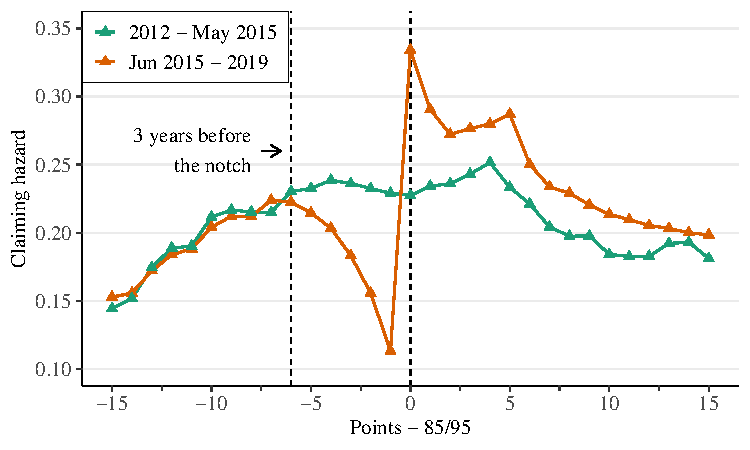
\includegraphics[width=.9\linewidth]{E3_claiming_haz_dist.pdf}
    % These are simulated points 
\end{frame}

\begin{frame}{DD: Efeito da Reforma no Hazard de Requerimento (CH)}
    \begin{itemize}
        \item $p$: pontos normalizados, ie, pontos - 85 (95) para mulheres (homens)
        \item Grupo de controle: agentes com $p<-6$ em $t$
        \item Grupos de tratamento: agentes com $p \in \tilde p$ em $t$ para $\tilde p=[-6,-3); [-3,0);[0,2);[2,7), [7,\infty)$
    \end{itemize}
    % Note that these are simulated points at each period t rather than points at claiming. 
    \begin{align*}
        CH_{ipt} = \sum_{k \neq -2} \beta_{k,\tilde p} 1(p \in \tilde p) \times 1(t = k) + \delta_t + \gamma_{p} +\zeta X_{ip} + \varepsilon_{ipt}
    \end{align*}
    \begin{itemize}
        \item $\beta_{k,\tilde p}$: efeito da reforma sobre o CH em $p\in \tilde p$
        \item $\delta_t$, $\gamma_{p}$: efeitos fixos de tempo e de pontos normalizados
        \item $X_{ip}$ inclui efeitos fixos de gênero, microrregião, escolaridade, raça e ano de nascimento (no momento do requerimento)
    \end{itemize}
\end{frame}

\begin{frame}{Efeito Negativo na CH Logo Abaixo do Limite $p\in [-2,0)$}
    \centering
    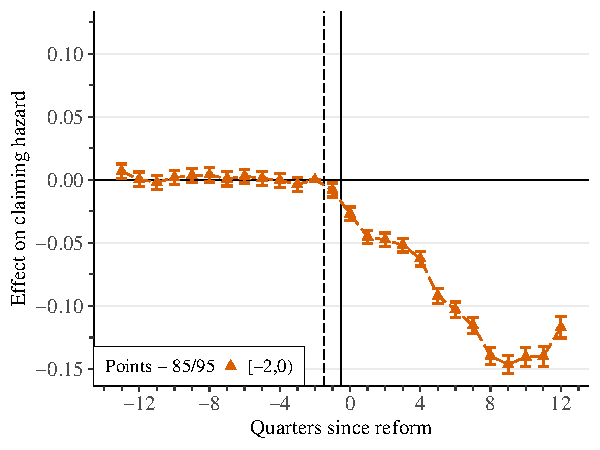
\includegraphics[width=0.8\linewidth]{F4_eventstudy_agg_2.pdf}
\end{frame}

\begin{frame}[label=ChDdRightAbove]{Efeito Positivo na CH Logo Acima do Limite $p \in[0,2)$}
    \centering
    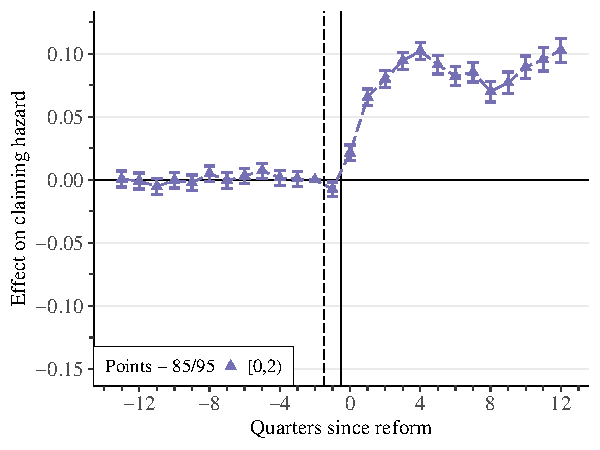
\includegraphics[width=0.8\linewidth]{F4_eventstudy_agg_3.pdf}
    \bfootnote{\hyperlink{chDdOther}{\beamerbutton{Outras Faixas de Pontos}} \hyperlink{trend}{\beamerbutton{Tendências Brutas}}\hyperlink{chToFrequencies}{\beamerbutton{CH para Frequências}}}
\end{frame}

\begin{frame}{Frequências Observadas e Contrafactuais
    \only<1>{Q4 2014}\only<2>{Q1 2015}\only<3>{Q2 2015}\only<4>{Q3 2015}\only<5>{Q4 2015}\only<6>{Q1 2016}\only<7>{Q2 2016}\only<8>{Q3 2016}\only<9>{Q4 2016}\only<10>{Q1 2017}\only<11>{Q2 2017}\only<12>{Q3 2017}\only<13>{Q4 2017}\only<14>{Q1 2018}\only<15>{Q2 2018}\only<16>{Q3 2018}}
     \centering \only<1>{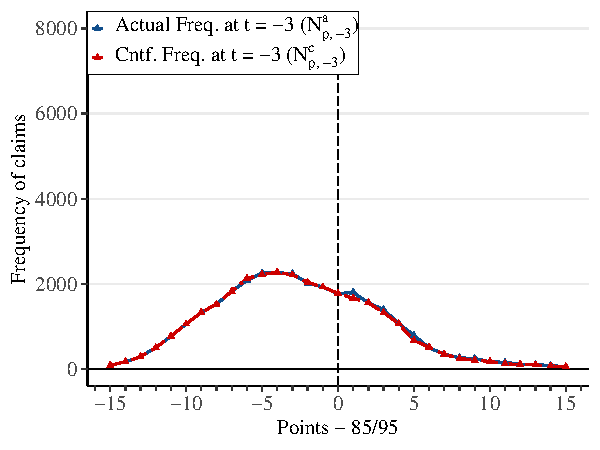
\includegraphics[width=.9\linewidth]{frequenciesQ-3.pdf}}\only<2>{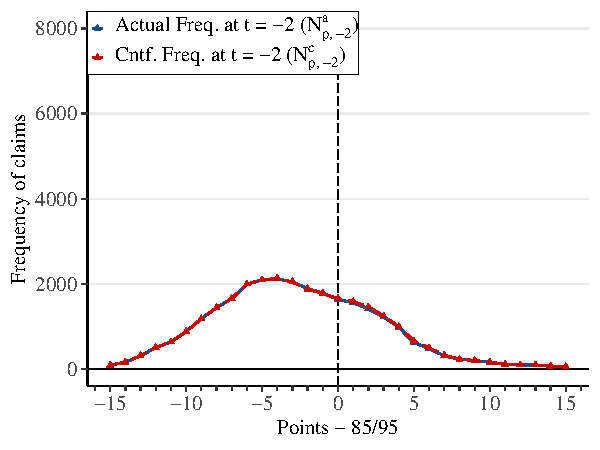
\includegraphics[width=.9\linewidth]{frequenciesQ-2.pdf}}\only<3>{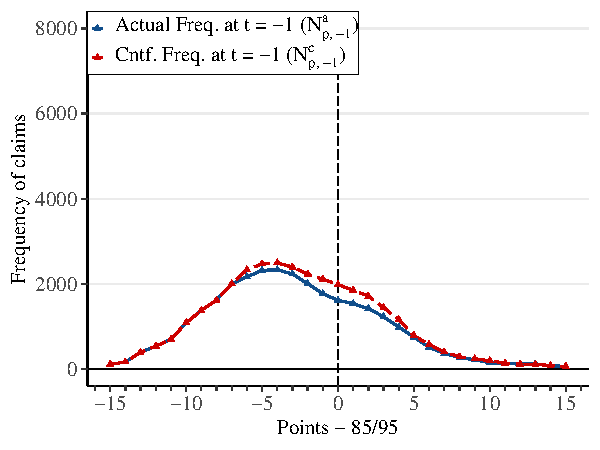
\includegraphics[width=.9\linewidth]{frequenciesQ-1.pdf}}\only<4>{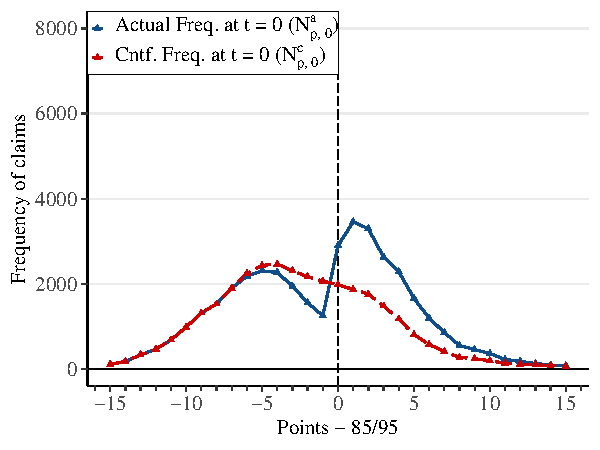
\includegraphics[width=.9\linewidth]{frequenciesQ0.pdf}}\only<5>{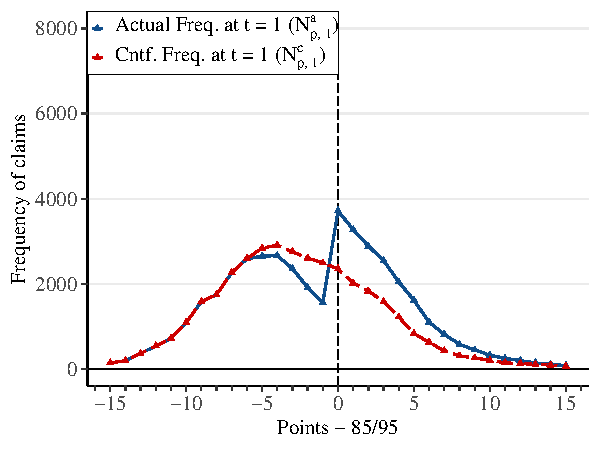
\includegraphics[width=.9\linewidth]{frequenciesQ1.pdf}}\only<6>{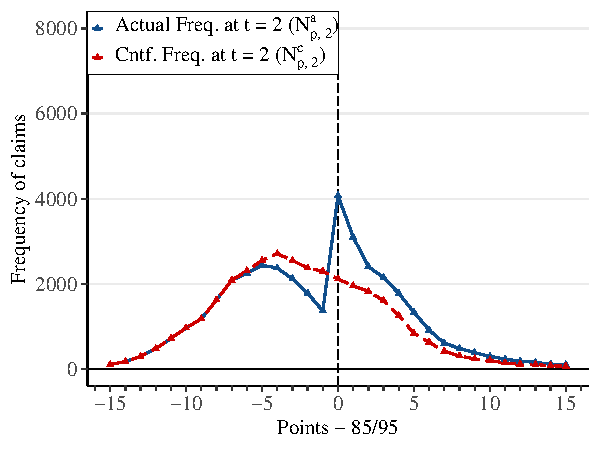
\includegraphics[width=.9\linewidth]{frequenciesQ2.pdf}}\only<7>{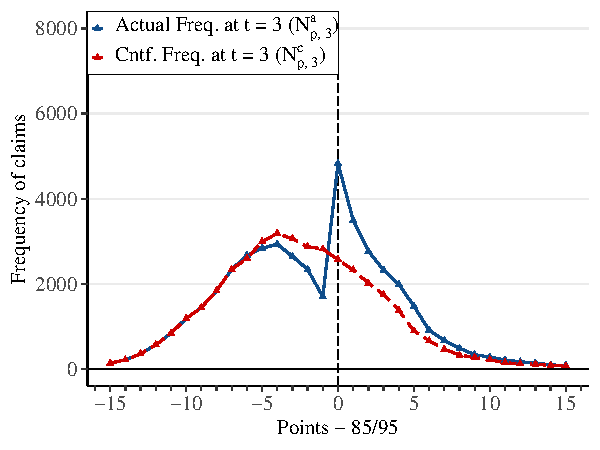
\includegraphics[width=.9\linewidth]{frequenciesQ3.pdf}}\only<8>{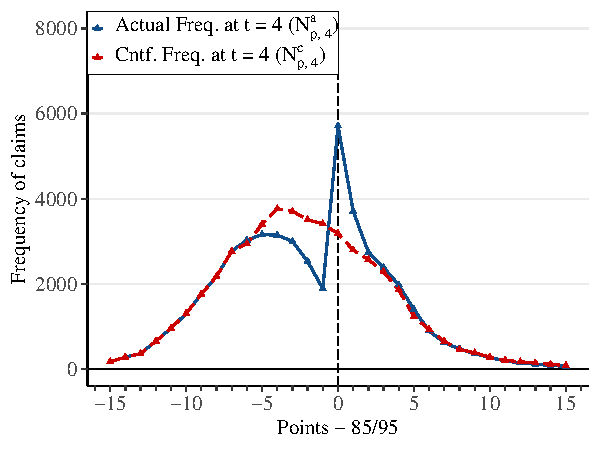
\includegraphics[width=.9\linewidth]{frequenciesQ4.pdf}}\only<9>{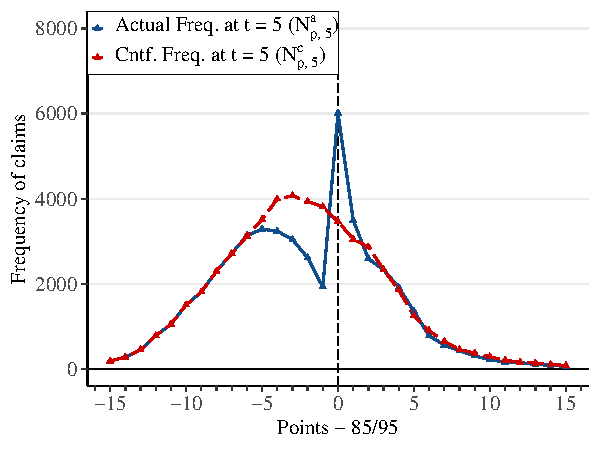
\includegraphics[width=.9\linewidth]{frequenciesQ5.pdf}}\only<10>{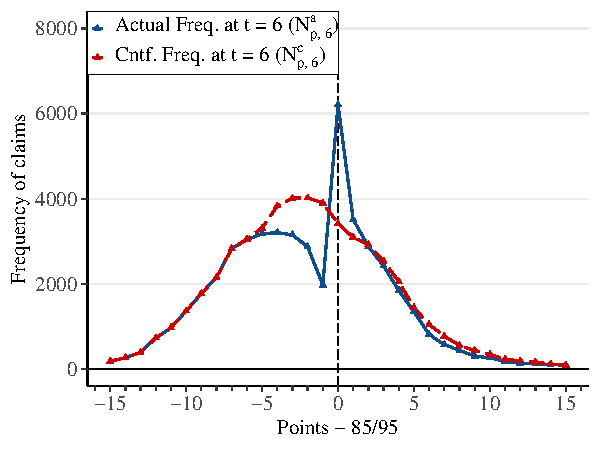
\includegraphics[width=.9\linewidth]{frequenciesQ6.pdf}}\only<11>{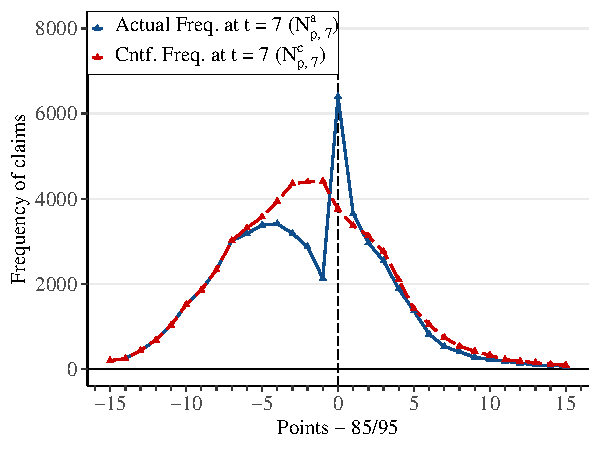
\includegraphics[width=.9\linewidth]{frequenciesQ7.pdf}}\only<12>{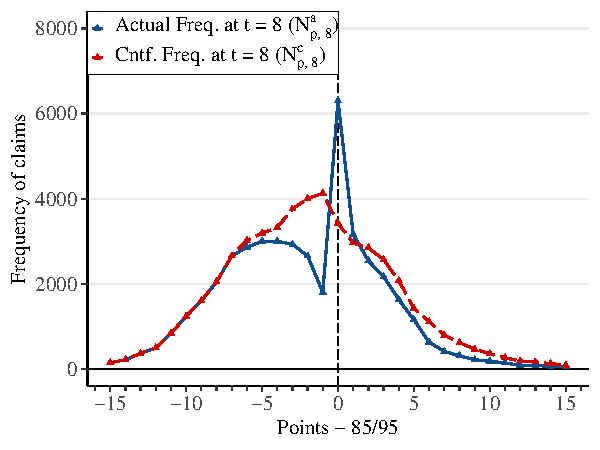
\includegraphics[width=.9\linewidth]{frequenciesQ8.pdf}}\only<13>{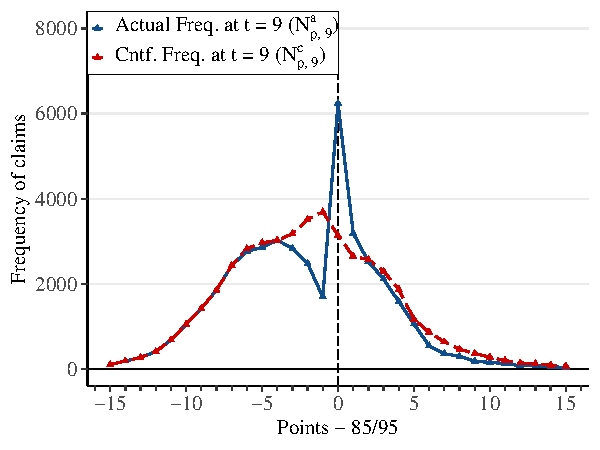
\includegraphics[width=.9\linewidth]{frequenciesQ9.pdf}}\only<14>{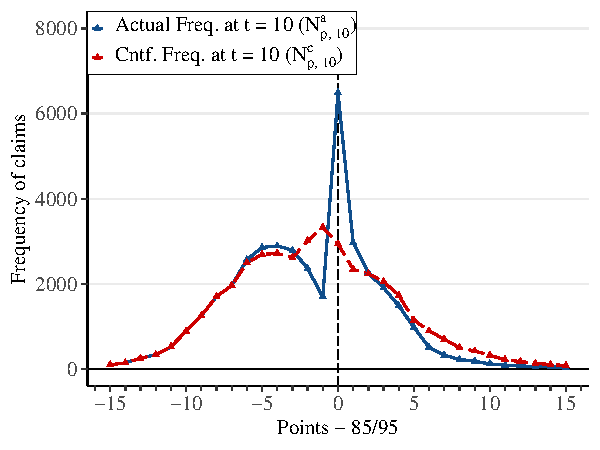
\includegraphics[width=.9\linewidth]{frequenciesQ10.pdf}}\only<15>{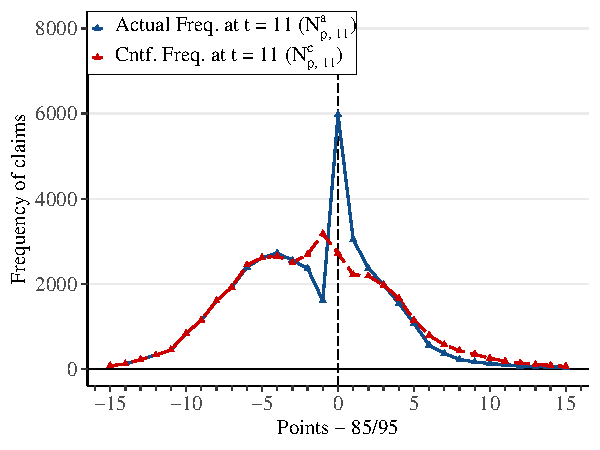
\includegraphics[width=.9\linewidth]{frequenciesQ11.pdf}}\only<16>{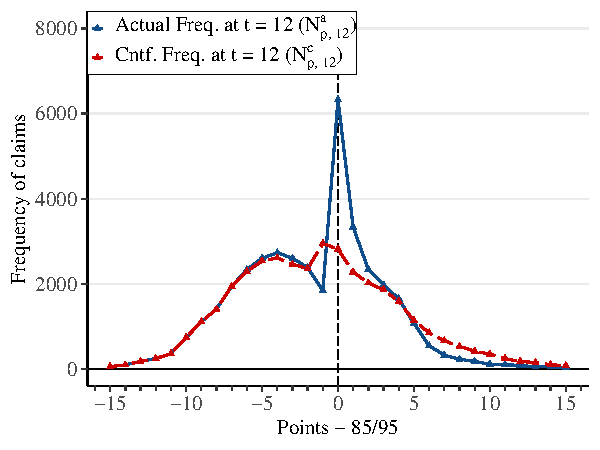
\includegraphics[width=.9\linewidth]{frequenciesQ12.pdf}}
\end{frame}

\begin{frame}[label=empiricalOverviewDAP]{Estratégia Empírica: Visão Geral}
\begin{itemize}
    \item Qual foi o efeito de bem-estar da reforma? O objetivo é calcular o MVPF (Marginal Value of Public Funds)
    \item[] $\Rightarrow$  Fazemos isso em quatro etapas:
    \begin{enumerate}
        \item Estimar como a reforma afetou a distribuição de pontos
        %\item Medir o valor presente dos benefícios vitalícios líquidos de impostos
        \item \textbf{Estimar o efeito mecânico no valor presente dos benefícios (DAP)}
        \item {Estimar o custo total da reforma}
        \item Medir o efeito de bem-estar da reforma e construir seu (W)MVPF
    \end{enumerate}
\end{itemize}
\bfootnote{\hyperlink{npv}{\beamerbutton{VPD líquido de impostos}}}
\end{frame}

\begin{frame}[label=MEandFE]{Efeito Mecânico e Disposição a Pagar}
    \begin{itemize}
        \item A DAP é capturada pelo efeito mecânico (teorema do envelope)
    \end{itemize}
    {\small
    \begin{align*}
         \sum_i \sum_{t=0}^{T_i} \frac{E[b^a(x^c_{it})]-E[b^c(x_{it}^c)]}{(1+r)^t}
    \end{align*}
    }
    \begin{itemize}
        \item Efeito mecânico: aumento contrafactual dos gastos com benefícios sob a regra reformada, mas na ausência de respostas comportamentais
        \item Podemos recuperar $\sum_t b^a(\mathbf{x_{it}^a})/(1+r)^t$ e $\sum_t b^c(\mathbf{x_{it}^a})/(1+r)^t$, mas precisamos de:
        \begin{enumerate}
            \item benefícios contrafactuais $\sum_t b^c(\mathbf{x_{it}^c})/(1+r)^t$
            \item benefícios mecânicos $\sum_t b^a(\mathbf{x^c_{it}})/(1+r)^t$
        \end{enumerate}
        \item Com as frequências contrafactuais de requerimento, só precisamos dos benefícios médios contrafactuais e mecânicos em cada $p$
    \end{itemize}
\end{frame}

\begin{frame}{Benefícios Contrafactuais Médios: $\frac{1}{N_{p,t}^c}\sum_{i:p(x_{it})=p}\sum_t \frac{b^c(x_{it}^c)}{(1+r)^t}$}
% This should be the sum of the PDV (from the perpective of the refomr) of benefits for those who claim at t with p points from t=0 to T_i.
% So p(x_it) = p only if i claims at t with p. 
    \begin{itemize}
        \item $\bar{b}^{c,a}_{p,t} \equiv \frac{1}{N_{p,t}} \sum_{i:p(x_{it}^a)=p}\sum_t b^c(x_{it}^a)/(1+r)^t$: VPD médio dos benefícios que teriam sido pagos aos que requerem com $p$ pontos normalizados no trimestre $t$ sob a regra contrafactual e as escolhas observadas
        \item Problema: os \textit{bunchers} podem ser positivamente selecionados (por exemplo, salários mais altos)
        \item Hipótese de identificação: $\bar{b}^{c,a}_{p,t}$ para $p\geq -6$ permaneceria paralelo ao observado em $p<-6$ na ausência da reforma
        \item O DiD recupera o efeito da reforma sobre esses benefícios médios $\beta^{c,a}_{k,p}$ em cada ponto normalizado $p$ e trimestre $k$:
         \begin{align*}
            \bar{b}^{c,a}_{p,t}=\delta_p^{c,a}+\gamma_t^{c,a} +\sum_{k\neq -2}\beta_{p,k}^{c,a} 1(p\in \tilde p)*1(t=k)+\varepsilon_{p,t}^{c,a}
        \end{align*}
        \item $\bar{b}^{c,a}_{p,t}-\hat \beta_{p,t}^{c,a}$ é uma estimativa de $\frac{1}{N_{p,t}^c}\sum_{i:p(x_{it})=p}\sum_t \frac{b^c(x^c_{it})}{(1+r)^t}$
    \end{itemize}
    % The estimate for the average benefit that would have been paid in the absence of the reform at point p and quarter t is estimated as bar b^o_{p,t}-\beta_{t,p}
\end{frame}

\begin{frame}{Efeito nos Benefícios Contrafs. Médios em $p \in [-2,0)$}
    \centering
    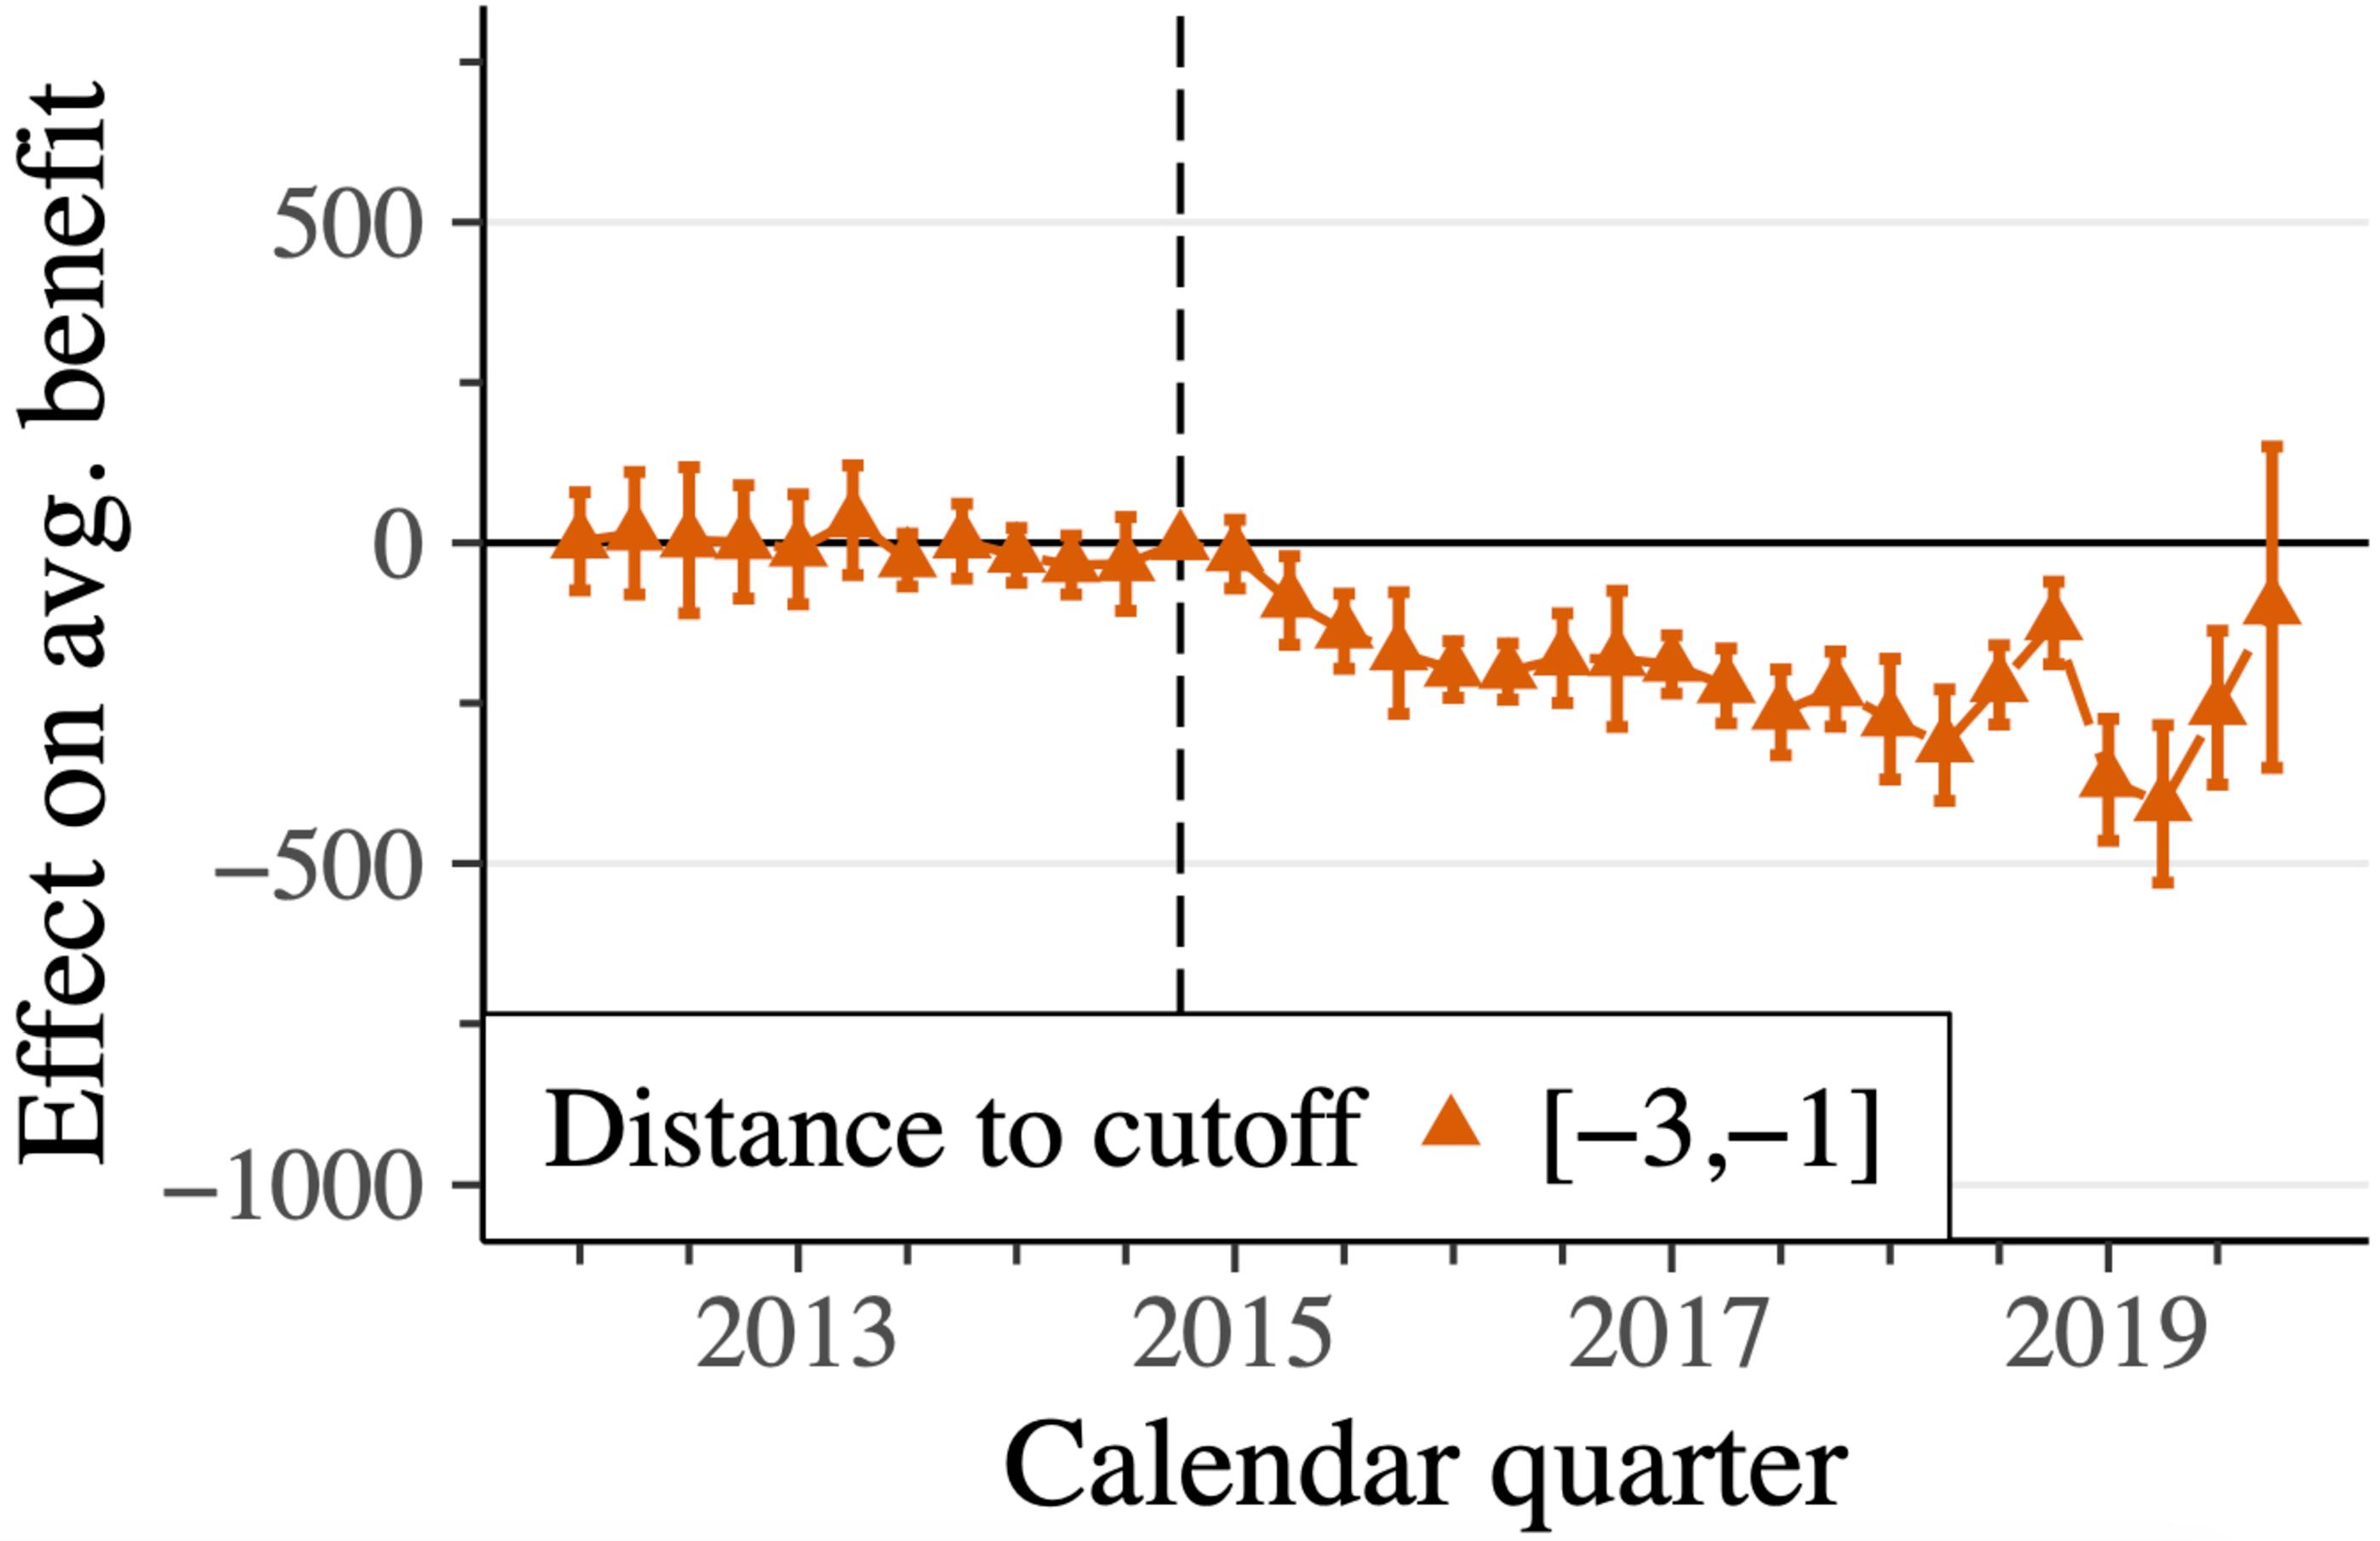
\includegraphics[width=0.8\linewidth]{old-3.pdf}
\end{frame}

\begin{frame}[label=selectionRightAbove]{Efeito nos Benefícios Contrafactuais Médios em $p \in [0,2)$}
    \centering
    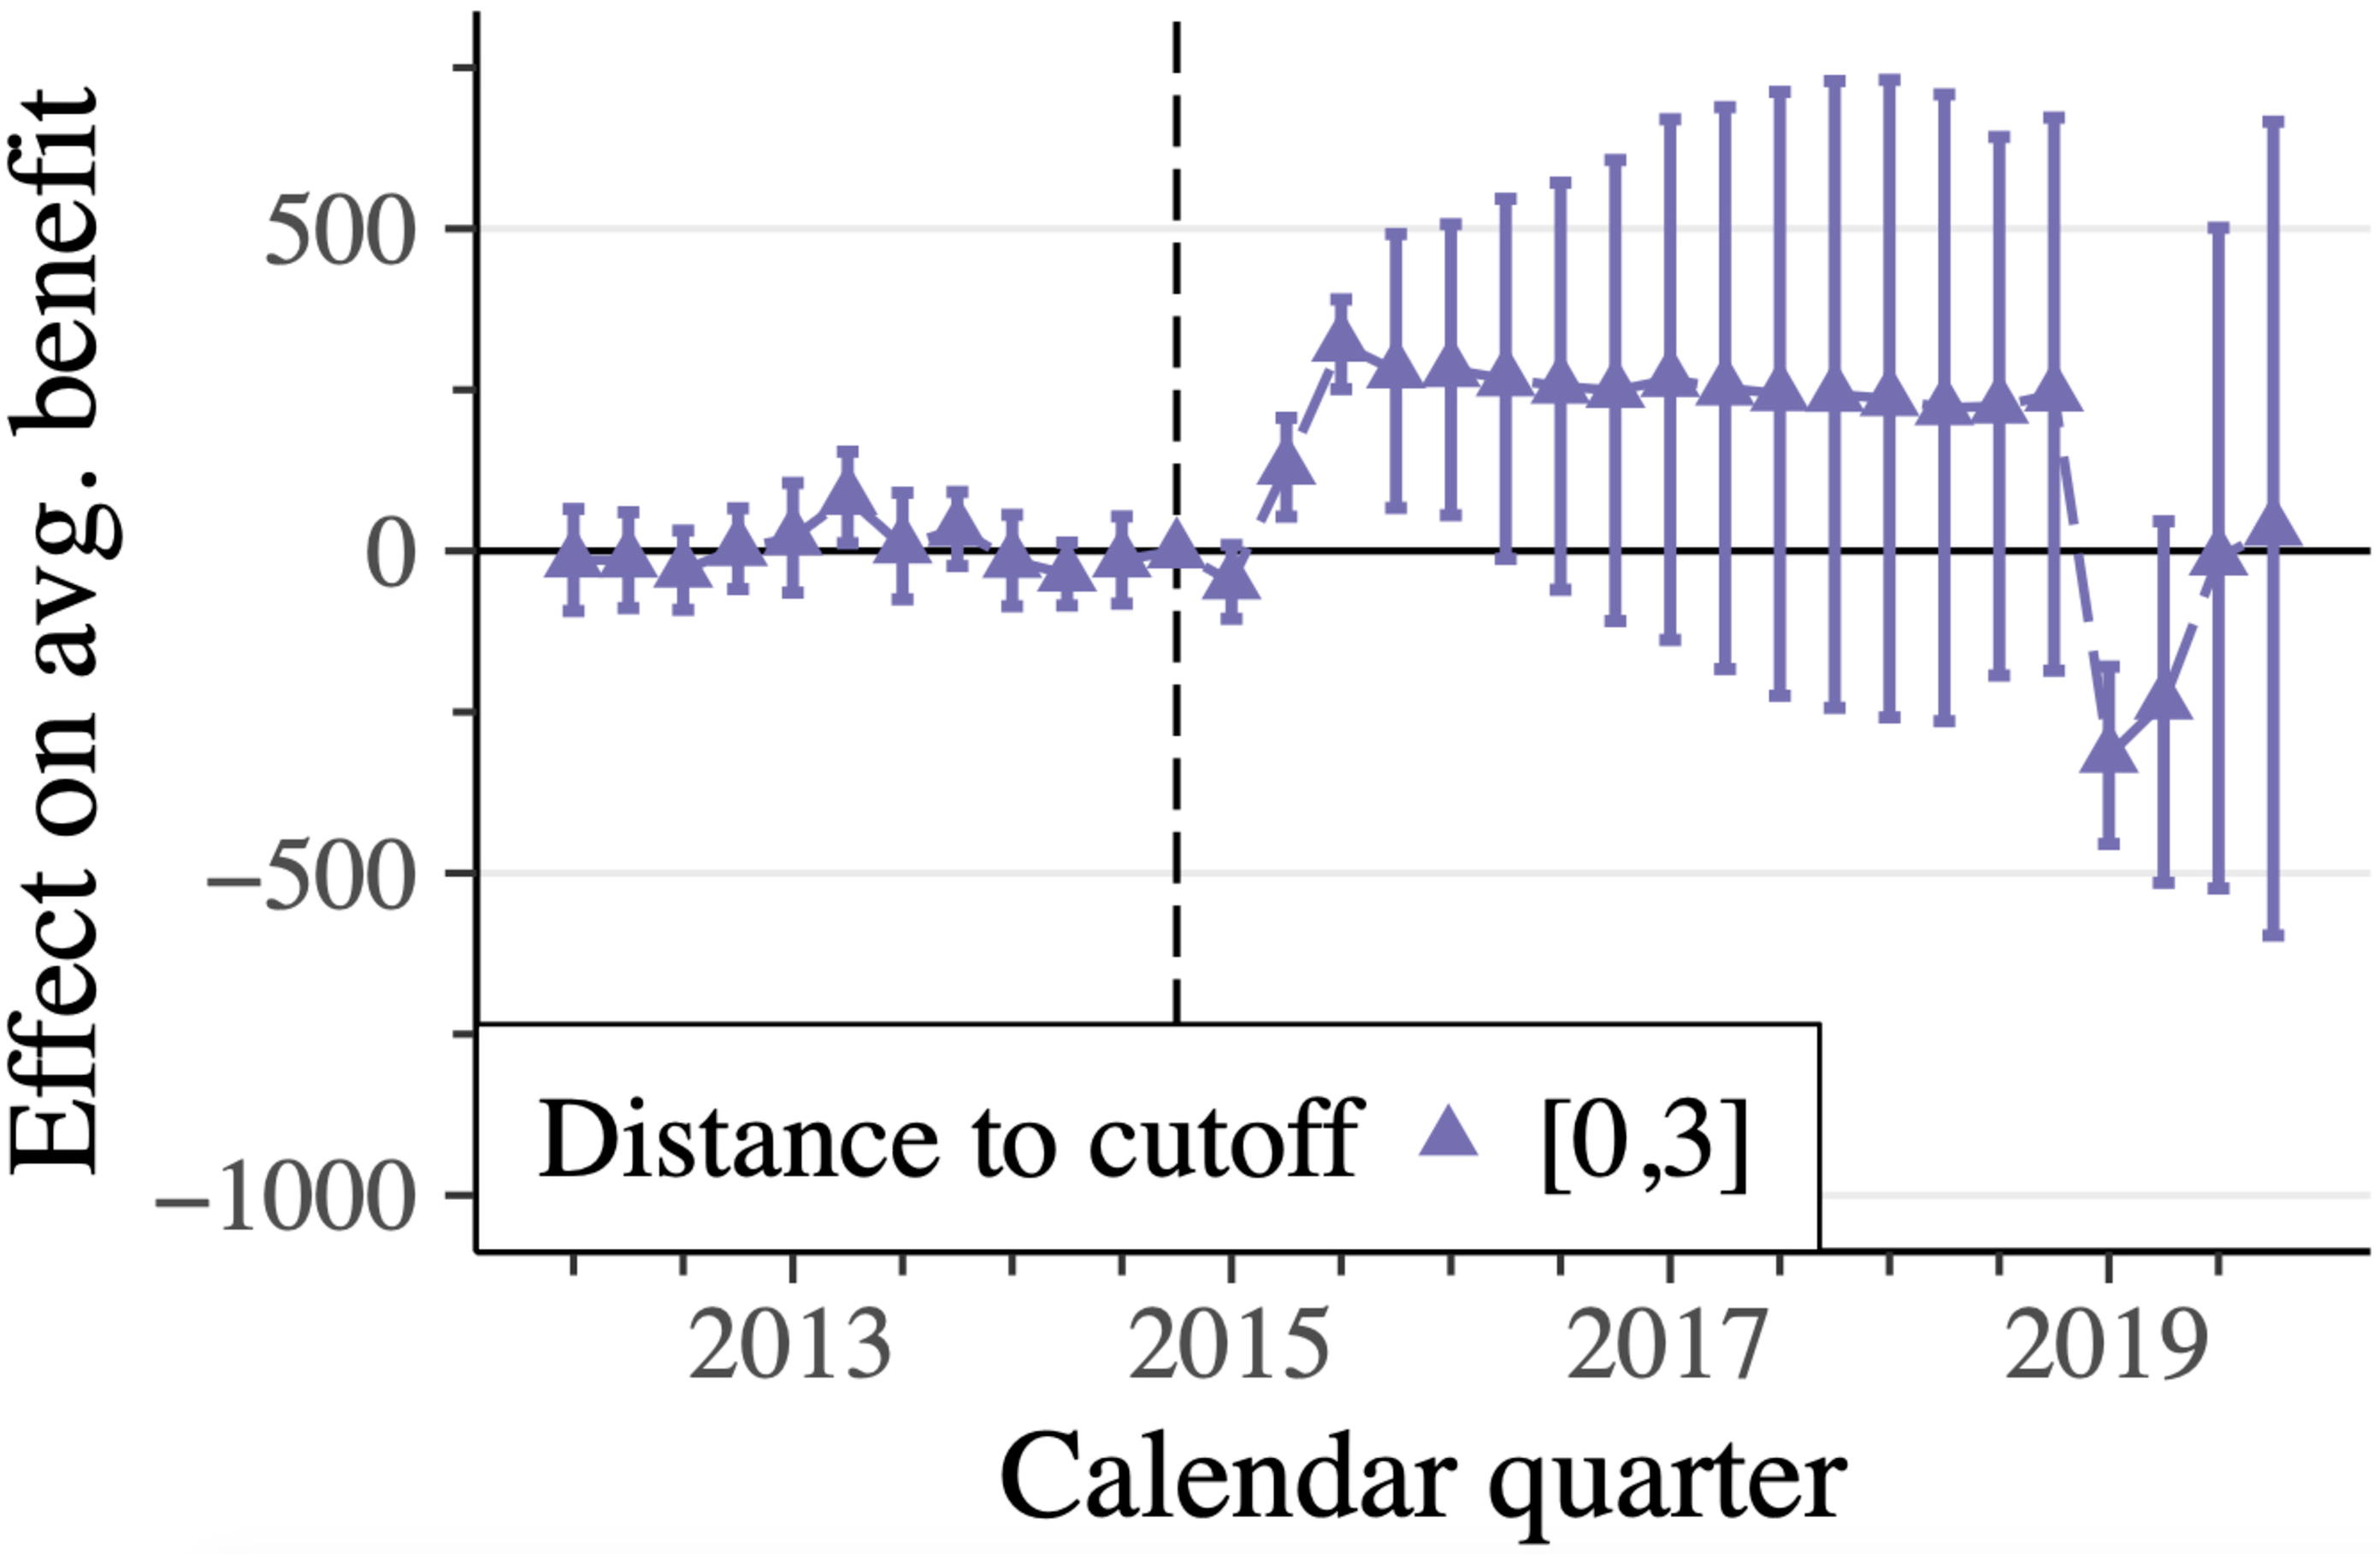
\includegraphics[width=0.8\linewidth]{old0.pdf}
    \bfootnote{\hyperlink{selectionOther}{\beamerbutton{Outras Faixas de Pontos}}}
\end{frame}


\begin{frame}{Benefícios Mecânicos Médios: $\frac{1}{N^c_{p,t}}\sum_{i:p(x_{it})=p} \sum_t \frac{b^a(x_{it}^c)}{(1+r)^t}$}
    \begin{itemize}
        %\item We correct the observed benefit outlay in each point $p$ and quarter $t$ by the selection of individuals that responded to the reform
        \item $\bar{b}^{a,a}_{p,t} \equiv \frac{1}{N_{p,t}}\sum_{i:p(x_{it}^a)=p}\sum_t \frac{b^a(x_{it}^a)}{(1+r)^t}$: VPD médio dos benefícios pagos aos que requerem com $p$ em $t$ sob a regra e escolhas observadas $\Rightarrow$ é preciso corrigir pelas respostas comportamentais
        \item Hipótese de identificação: $\bar{b}^{a,a}_{p,t}$ para $p\geq -6$ permaneceria paralelo ao observado em $p<-6$ na ausência da reforma
        \item O DiD a seguir recupera o efeito da reforma sobre esses benefícios médios $\beta^{a,a}_{k,p}$ em cada ponto normalizado $p$ e trimestre $k$:
         \begin{align*}
            \bar{b}^{a,a}_{p,t}=\delta_p^{a,a}+\gamma_t^{a,a} +\sum_{k\neq -2}\beta_{k,p}^{a,a} 1(p\in \tilde p)*1(t=k)+\varepsilon_{p,t}^{a,a}
        \end{align*}
        \item $\bar{b}^{a,a}_{p,t}-\hat \beta_{p,t}^{a,a}$ é uma estimativa de $\frac{1}{N^c_{p,t}}\sum_{i:p(x_{it})=p}\sum_t \frac{b^a(x^c_{it})}{(1+r)^t}$
    \end{itemize}
\end{frame}

\begin{frame}{Efeito sobre os Benefícios Observados Médios em $p \in [-2,0)$}
    \centering
    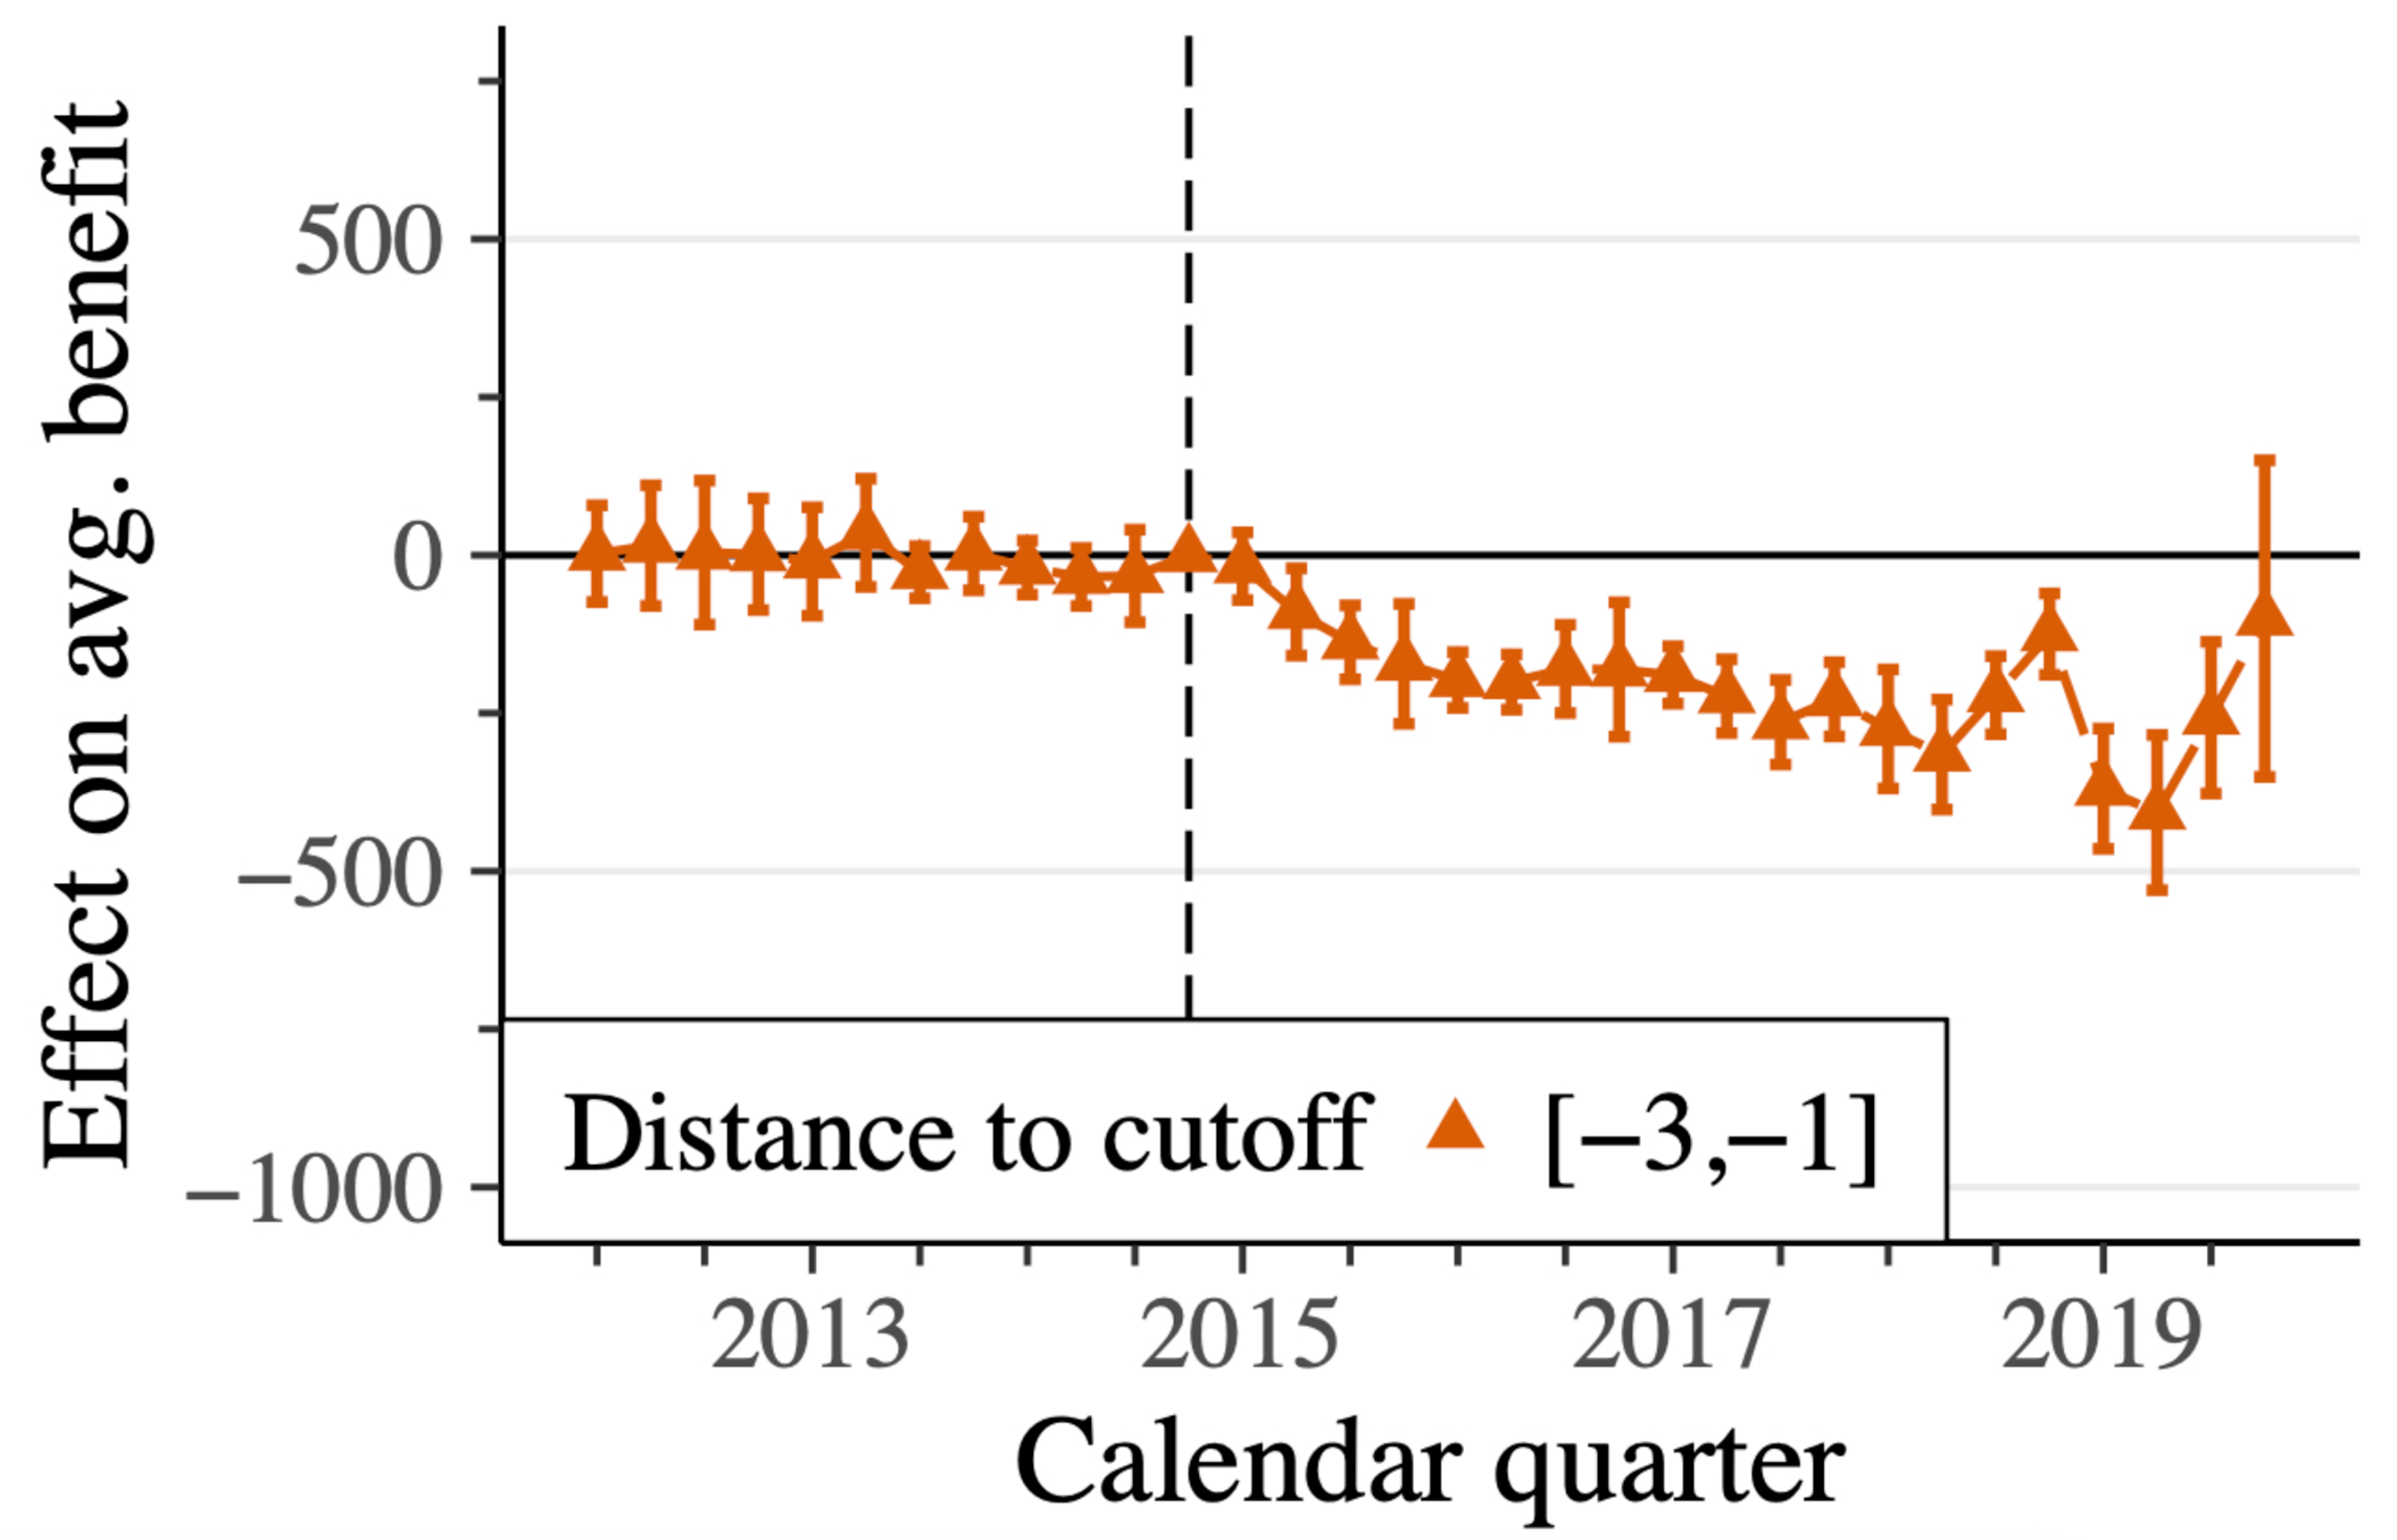
\includegraphics[width=0.8\linewidth]{new-3.pdf}
\end{frame}

\begin{frame}[label=mechanicalRightAbove]{Efeito sobre os Benefícios Observados Médios em $p \in [0,2)$}
    \centering
    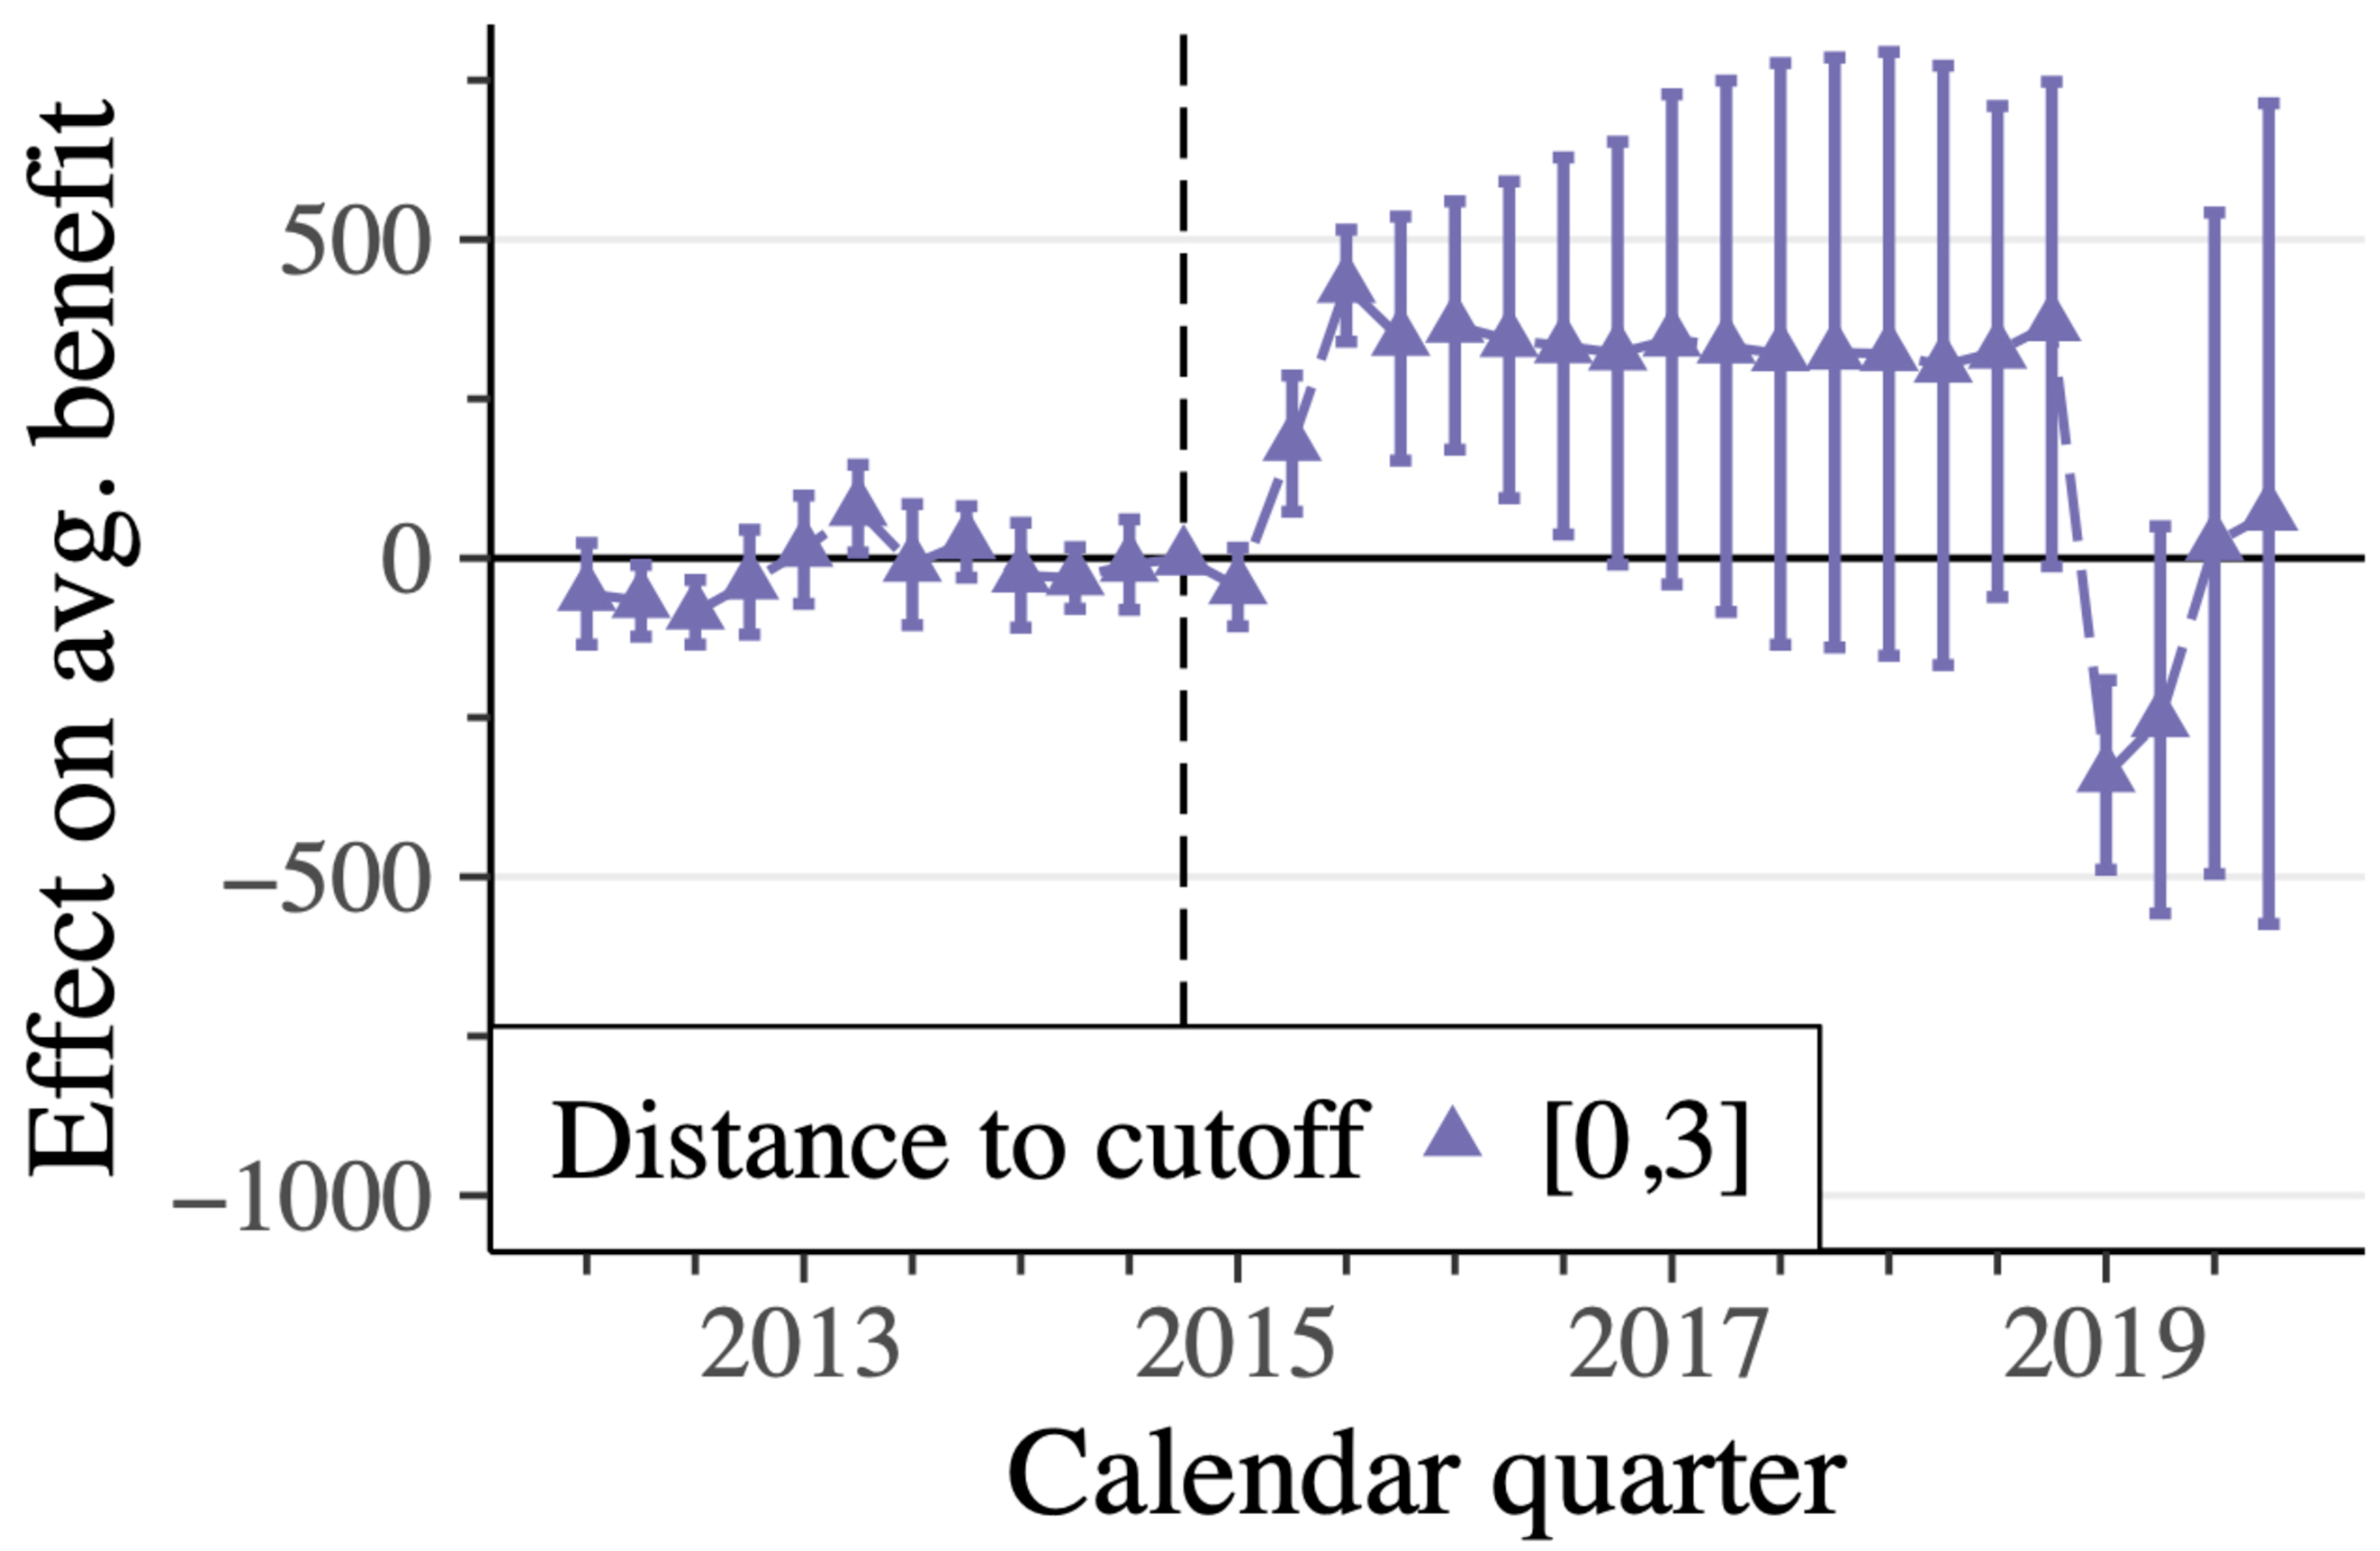
\includegraphics[width=0.8\linewidth]{new0.pdf}
    \bfootnote{\hyperlink{mechanicalOther}{\beamerbutton{Outras Faixas de Pontos}}}
\end{frame}

\begin{frame}{Estratégia Empírica: Visão Geral}
\begin{itemize}
    \item Qual foi o efeito de bem-estar da reforma? O objetivo é calcular o MVPF (Marginal Value of Public Funds)
    \item[] $\Rightarrow$  Fazemos isso em quatro etapas:
    \begin{enumerate}
        \item Estimar como a reforma afetou a distribuição de pontos
        %\item Medir o valor presente dos benefícios vitalícios líquidos de impostos
        \item {Estimar o efeito mecânico no valor presente dos benefícios (DAP)}
        \item \textbf{Estimar o custo total da reforma}
        \item Medir o efeito de bem-estar da reforma e construir seu (W)MVPF
    \end{enumerate}
\end{itemize}
\end{frame}

\begin{frame}[label=costReform]{Custo da Reforma}
    \begin{itemize}
        \item O custo total da reforma é
    \end{itemize}
    \only<1>{\small
    \begin{align*}
        \small
        \sum_{t=0}^T \sum_i \frac{E[b^a(x_{it}^a)-\tau(x_{it}^a)]-E[b^c(x^c_{it})-\tau(x_{it}^c)]}{(1+r)^t}
    \end{align*}
    }
    \only<2>{\small
    \begin{align*}
        \small
        \sum_{t=0}^T \sum_i \frac{E[b^a(x_{it}^a)]-E[b^c(x^c_{it})]}{(1+r)^t}
    \end{align*}
    }
    \begin{itemize}
        \item No período pós-reforma, os custos observados $b^a(x_{it}^a)-\tau(x_{it}^a)$ são diretamente observados, mas precisamos dos custos contrafactuais $b^c(x^c_{it})-\tau(x^c_{it})$
        \item Como temos as frequências contrafactuais de requerimento, só precisamos do benefício líquido de impostos contrafactual médio
        \item \only<1>{Hoje vamos apresentar resultados que ignoram as externalidades fiscais sobre a arrecadação tributária}\only<2>{\textbf{Hoje vamos apresentar resultados que ignoram as externalidades fiscais sobre a arrecadação tributária}}
    \end{itemize}
    \bfootnote{\hyperlink{netOfTaxBenefits}{\beamerbutton{Benefícios Contrafactuais Líquidos de Impostos}}}
\end{frame}

\begin{frame}{Estratégia Empírica: Visão Geral}
\begin{itemize}
    \item Qual foi o efeito de bem-estar da reforma? O objetivo é calcular o MVPF (Marginal Value of Public Funds)
    \item[] $\Rightarrow$  Fazemos isso em quatro etapas:
    \begin{enumerate}
        \item Estimar como a reforma afetou a distribuição de pontos
        %\item Medir o valor presente dos benefícios vitalícios líquidos de impostos
        \item {Estimar o efeito mecânico no valor presente dos benefícios (DAP)}
        \item {Estimar o custo total da reforma}
        \item \textbf{Medir o efeito de bem-estar da reforma e construir seu (W)MVPF}
    \end{enumerate}
\end{itemize}
\end{frame}

\begin{frame}{WMVPF e MVPF da Reforma}
    \begin{itemize}
        \item Sob as condições do envelope, o efeito de bem-estar por real gasto é:
        % It is an approximation because we are considering a non-infinitesimal reform
        \begin{align*}
            WMVPF(b^c,b^a)\approx \frac{\sum_t \sum_x E(SMU_{it}|x)*[b^a(x)-b^c(x)]}{C(b^c,b^a)}
        \end{align*}
        % technically, we are also holding constant the state of the world in b^a(x,pi). I believe we want the same distribution as in the absence of the reform. 
        % For example, if someone gets fired with a higher probability under the reformed schedule, we want to compute their benefits with the lower probability before the reform was enacted 
        \item Onde $E(SMU_{it}|x) \equiv E\left(\beta^t \frac{\partial u(x_{it})}{\partial c_{it}} \middle| x_{it}=x\right)$ é a utilidade marginal social média do consumo para agentes com escolhas $x$
        \item Supondo que os benefícios previdenciários não tenham valor de seguro e que não haja internalidades:
    \end{itemize}
    \begin{align*}
        MVPF & = \frac{\sum_t \sum_x E[b^a(x)-b^c(x)]}{C(b^c,b^a)} \\
        & = \frac{\text{Efeito Mecânico}}{\text{Custo Total}}
    \end{align*}
\end{frame}

\begin{frame}[label=consumptionApprox]{Medindo o Efeito de Bem-Estar da Reforma}
    \begin{itemize}
        \item Planejador utilitarista + normalização da utilidade marginal pela média da economia + CRRA constante:
        % CRRA constant across individuals, allow us to write gamma without i
        % CRRA constant across consumption levels allow us to use equal instead of approx
        \begin{align*}
            E(SMU_{it}|x) = \beta^{t}\left(1-\gamma\frac{c_{x}-c}{c}\right)
        \end{align*}
        \begin{itemize}
            \item $\gamma$ é o parâmetro de CRRA (assumido igual a 4), $c_x$ é o consumo médio entre os que escolhem $x$, e $c$ é o consumo médio da população brasileira
        \end{itemize}
        \item As evidências de pesquisa sugerem que o consumo é:
        \begin{enumerate}
            \item constant across points (ELSI)
            \item 4.2\% higher among beneficiaries than in the overall population (POF)
        \end{enumerate}
        % I also think we are using just the average c_x instead of c_x in the end
        % I think the correct thing to do is to use (c_x-c)*(b_x-b) and then sum..
        % This has to do with the jensen inequality
    \end{itemize}
\end{frame}

\begin{frame}[label=survey]{ELSI: Consumo por Pontos Normalizados}
    \centering 
    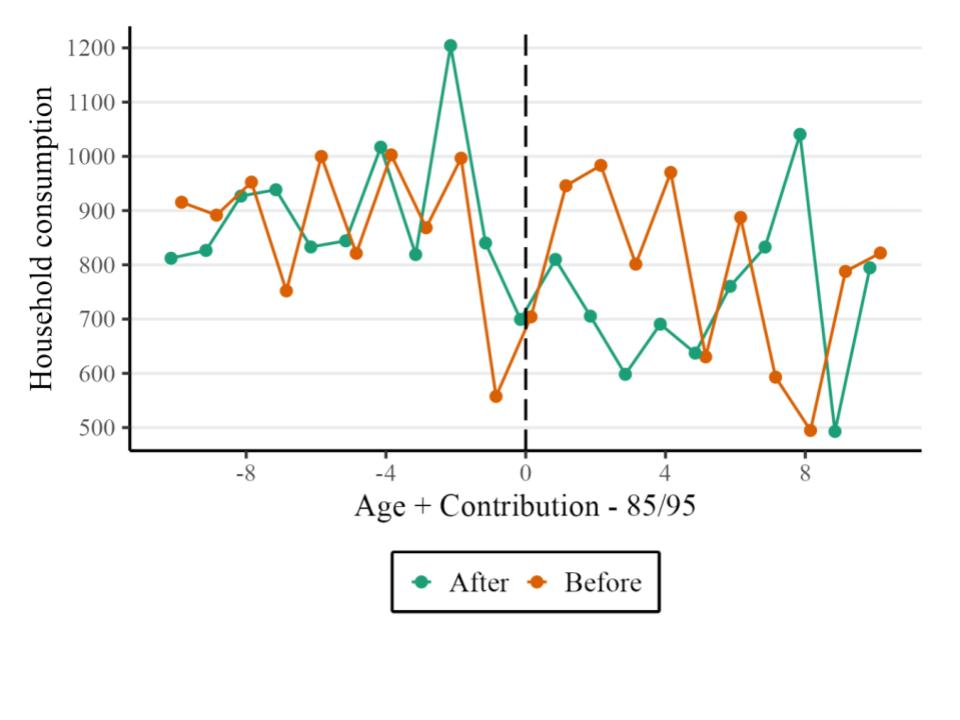
\includegraphics[width=\textwidth]{ELSI.jpg}
    % Roughly constant, 
    % It doesnt seem like redistribution within beneficiaries was that important
\end{frame}

\begin{frame}{Resultados da POF}
    \centering 
    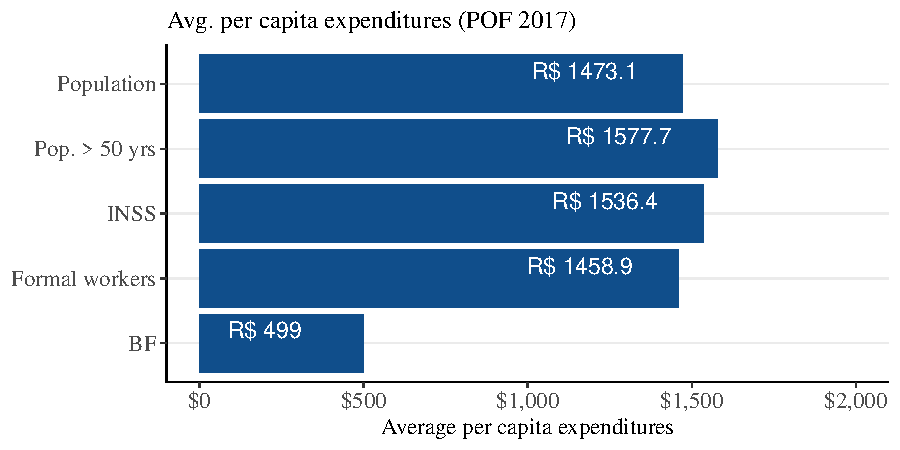
\includegraphics[width=\textwidth]{plot_expenditures_groups.pdf}
    % Pension beneficiaries consumed 8.2% more
    % Their marginal utility is therefore lower. 
    % Welfare effect < Mechanical effect
\end{frame}

\section{Efeito de Bem-Estar da Reforma}

\begin{frame}[label=welfareGraph]{MVPF Ponderado por Bem-Estar}
    \begin{figure}
        \centering
        \label{plot_wmvpf}
        %\caption{}
        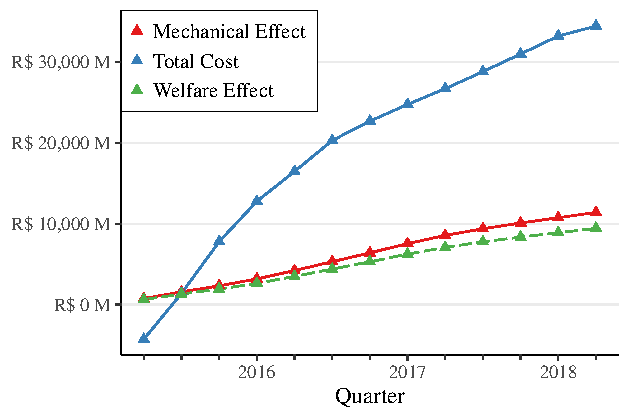
\includegraphics[width=0.8\linewidth]{plot_wmvpf.pdf}
    \end{figure}
    \begin{itemize}
        \item $WMVPF \approx 0.26$ (>3 para o BF)
    \end{itemize}
\end{frame}

\section{Separando Respostas a $\Delta b_L$ e $\Delta b_S$}

\begin{frame}[label=twoCounterfactualReforms]{Reforma Ótima e Duas Reformas Contrafactuais}
    \begin{itemize}
        \item A reforma ótima orçariamente neutra de $b()$ depende dos efeitos de bem-estar de $\Delta b_S()$ e $\Delta b_L()$ (Bergstrom et al, 2026)
        \begin{itemize}
            \item Aumentar o gasto no parâmetro com maior WMVPF
            \item Reduzir o gasto no parâmetro com menor WMVPF
        \end{itemize}
    \end{itemize}
    \centering
    \begin{minipage}[b]{0.47\textwidth}
        \centering
        %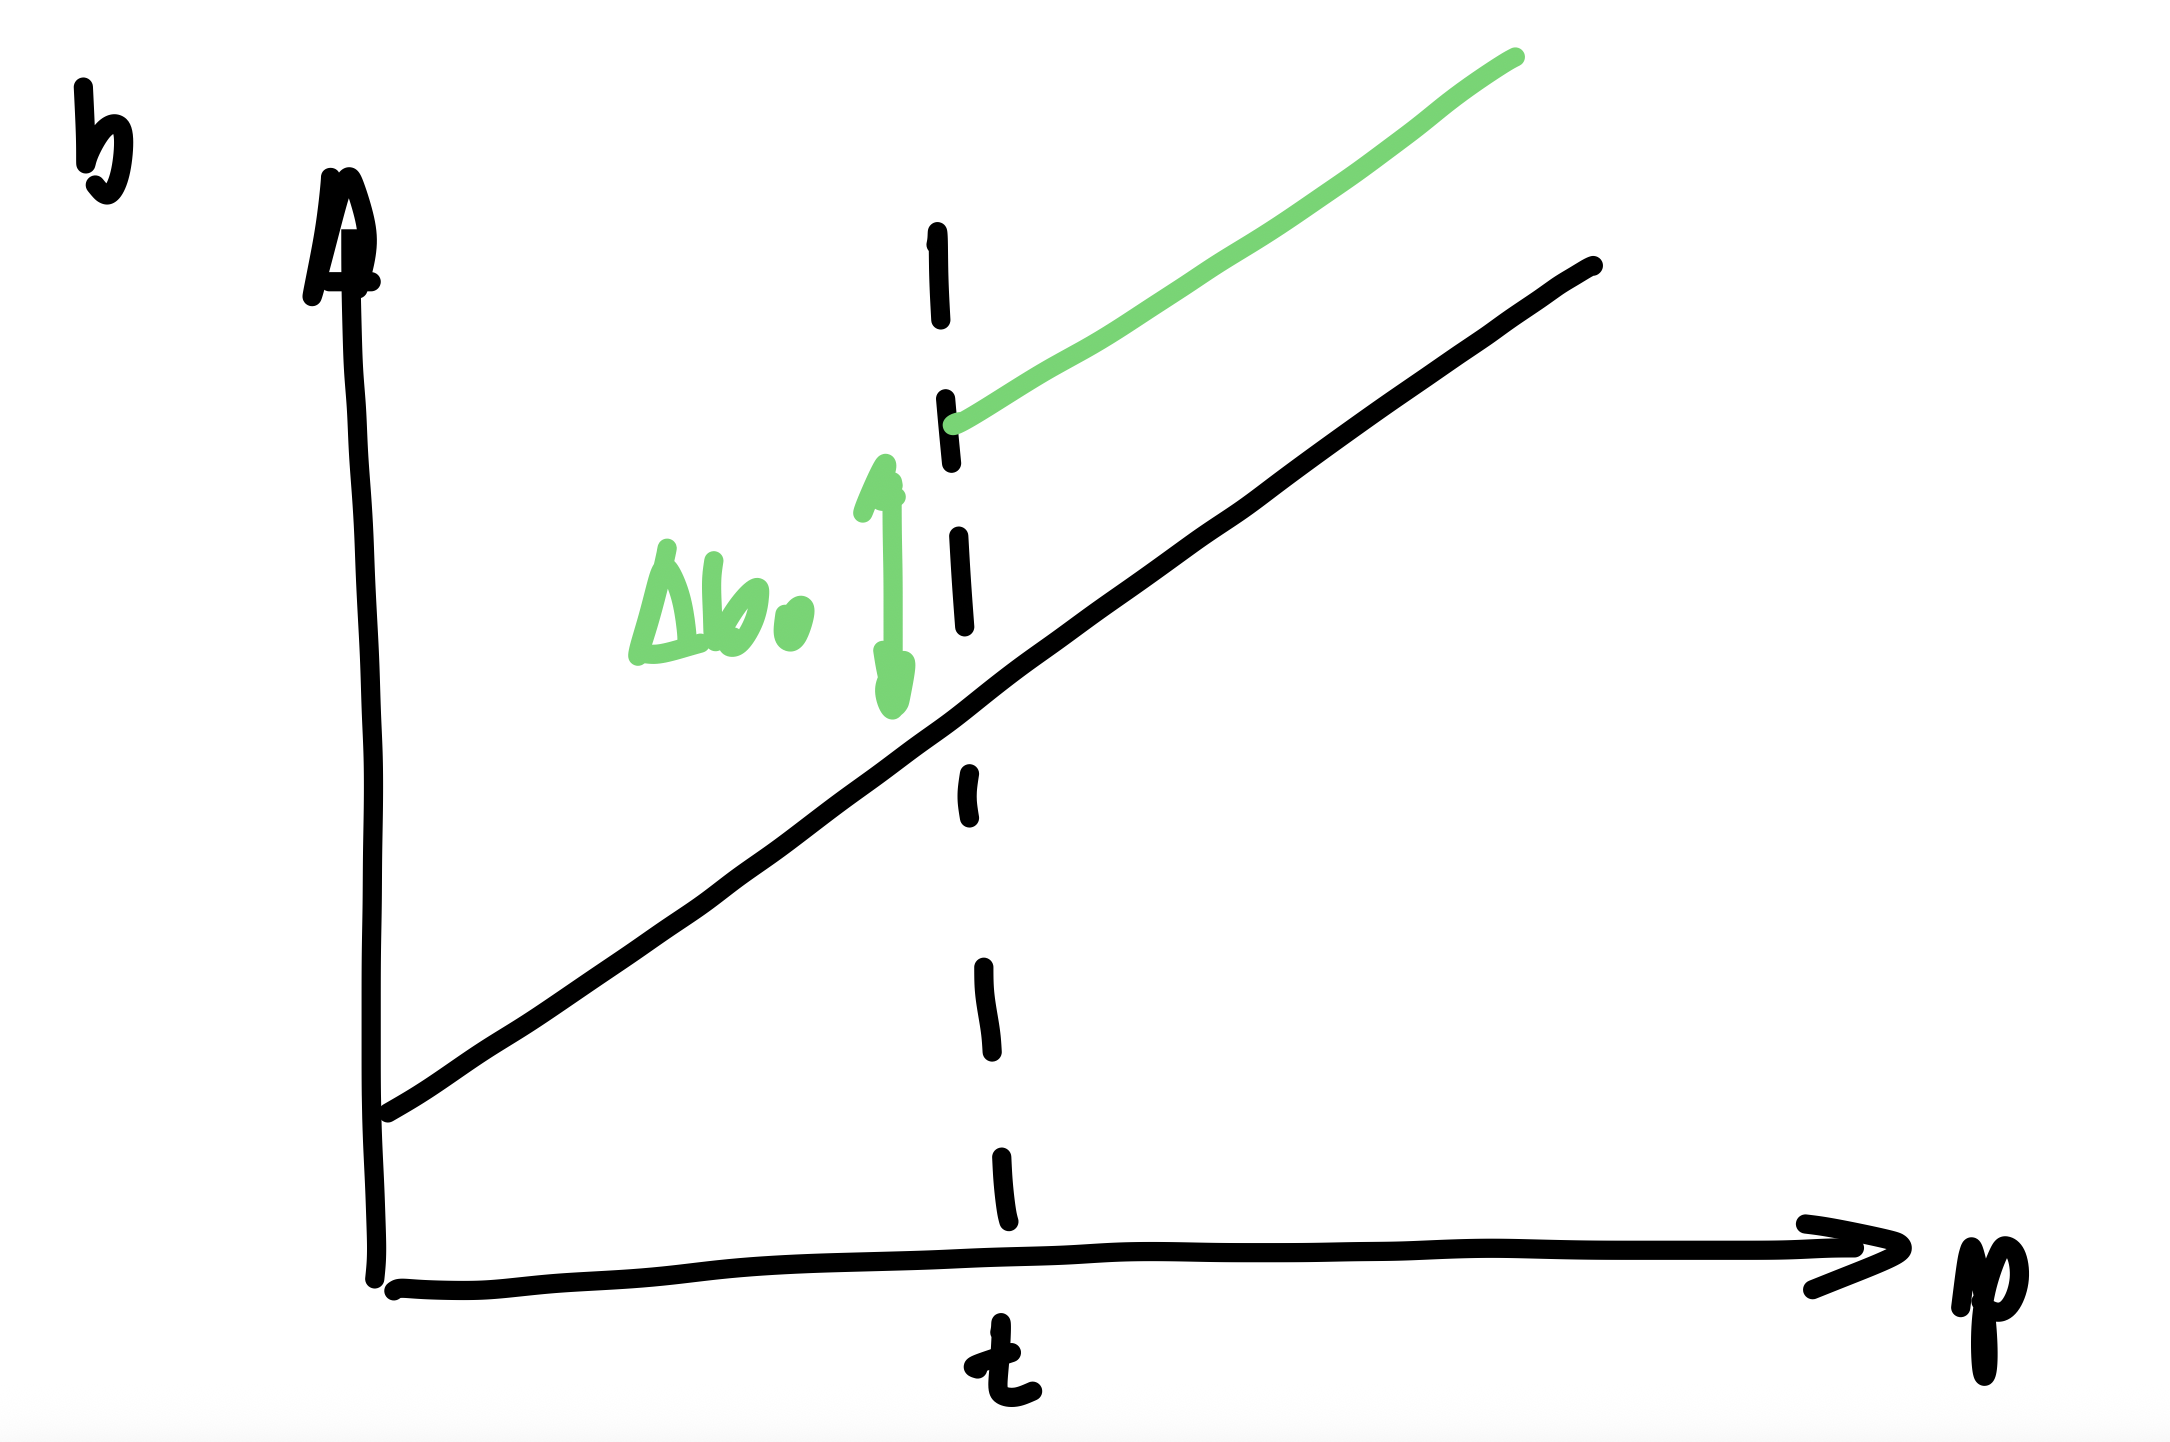
\includegraphics[width=\textwidth]{reformB0.png}
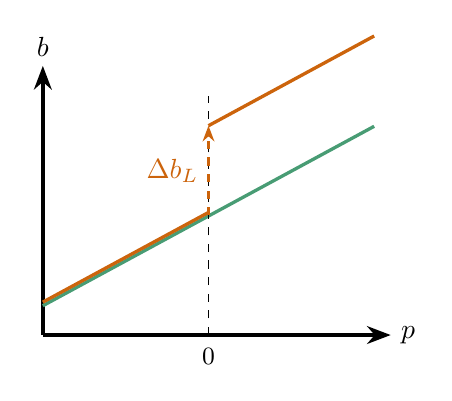
\begin{tikzpicture}
  \begin{axis}[
    width=6cm, height=5cm,
    axis lines=left,
    axis line style={-{Stealth[length=3mm]}, ultra thick},
    xmin=0, xmax=4.2, ymin=0, ymax=9,
    xtick=\empty, ytick=\empty, clip=false,
    xlabel={},
    xlabel style={at={(axis description cs:1.02,0)}, anchor=west},
    ylabel={},
  ]

    % Axis labels
    \node[anchor=south, rotate=0] at (axis description cs:0,1) {$b$};
    \node[anchor=south, rotate=0] at (axis description cs:1.05,-0.07) {$p$};

    % Black baseline line
    \addplot[very thick,col_before,domain=0:4] {0.98+1.5*x};

    % Green shifted line (parallel, upward shift)
    \addplot[very thick,col_after,domain=0:2] {1.1+1.5*x};

    % Green horizontal line
    \addplot[very thick,col_after,domain=2:4] {4 + 1.5*x};

    \draw[dashed,black!60!black] (axis cs:2,0) -- (axis cs:2,8);

    % Pick a reference point along the black line
    \coordinate (A) at (axis cs:2,{1+1.5*2});
    \coordinate (B) at (axis cs:2,7); % same x, higher y (on green line)

    % Dashed arrows showing Δb_ℓ (vertical) and Δb_s (horizontal)
    \draw[col_after, dashed, thick, -{Stealth[length=2mm]}] (A) -- (B) node[midway,left] {$\Delta b_L$};

    \node at (axis cs:{2},-0.7) {\small $0$};

  \end{axis}
\end{tikzpicture}
    \end{minipage}
    \begin{minipage}[b]{0.47\textwidth}
        \centering
        %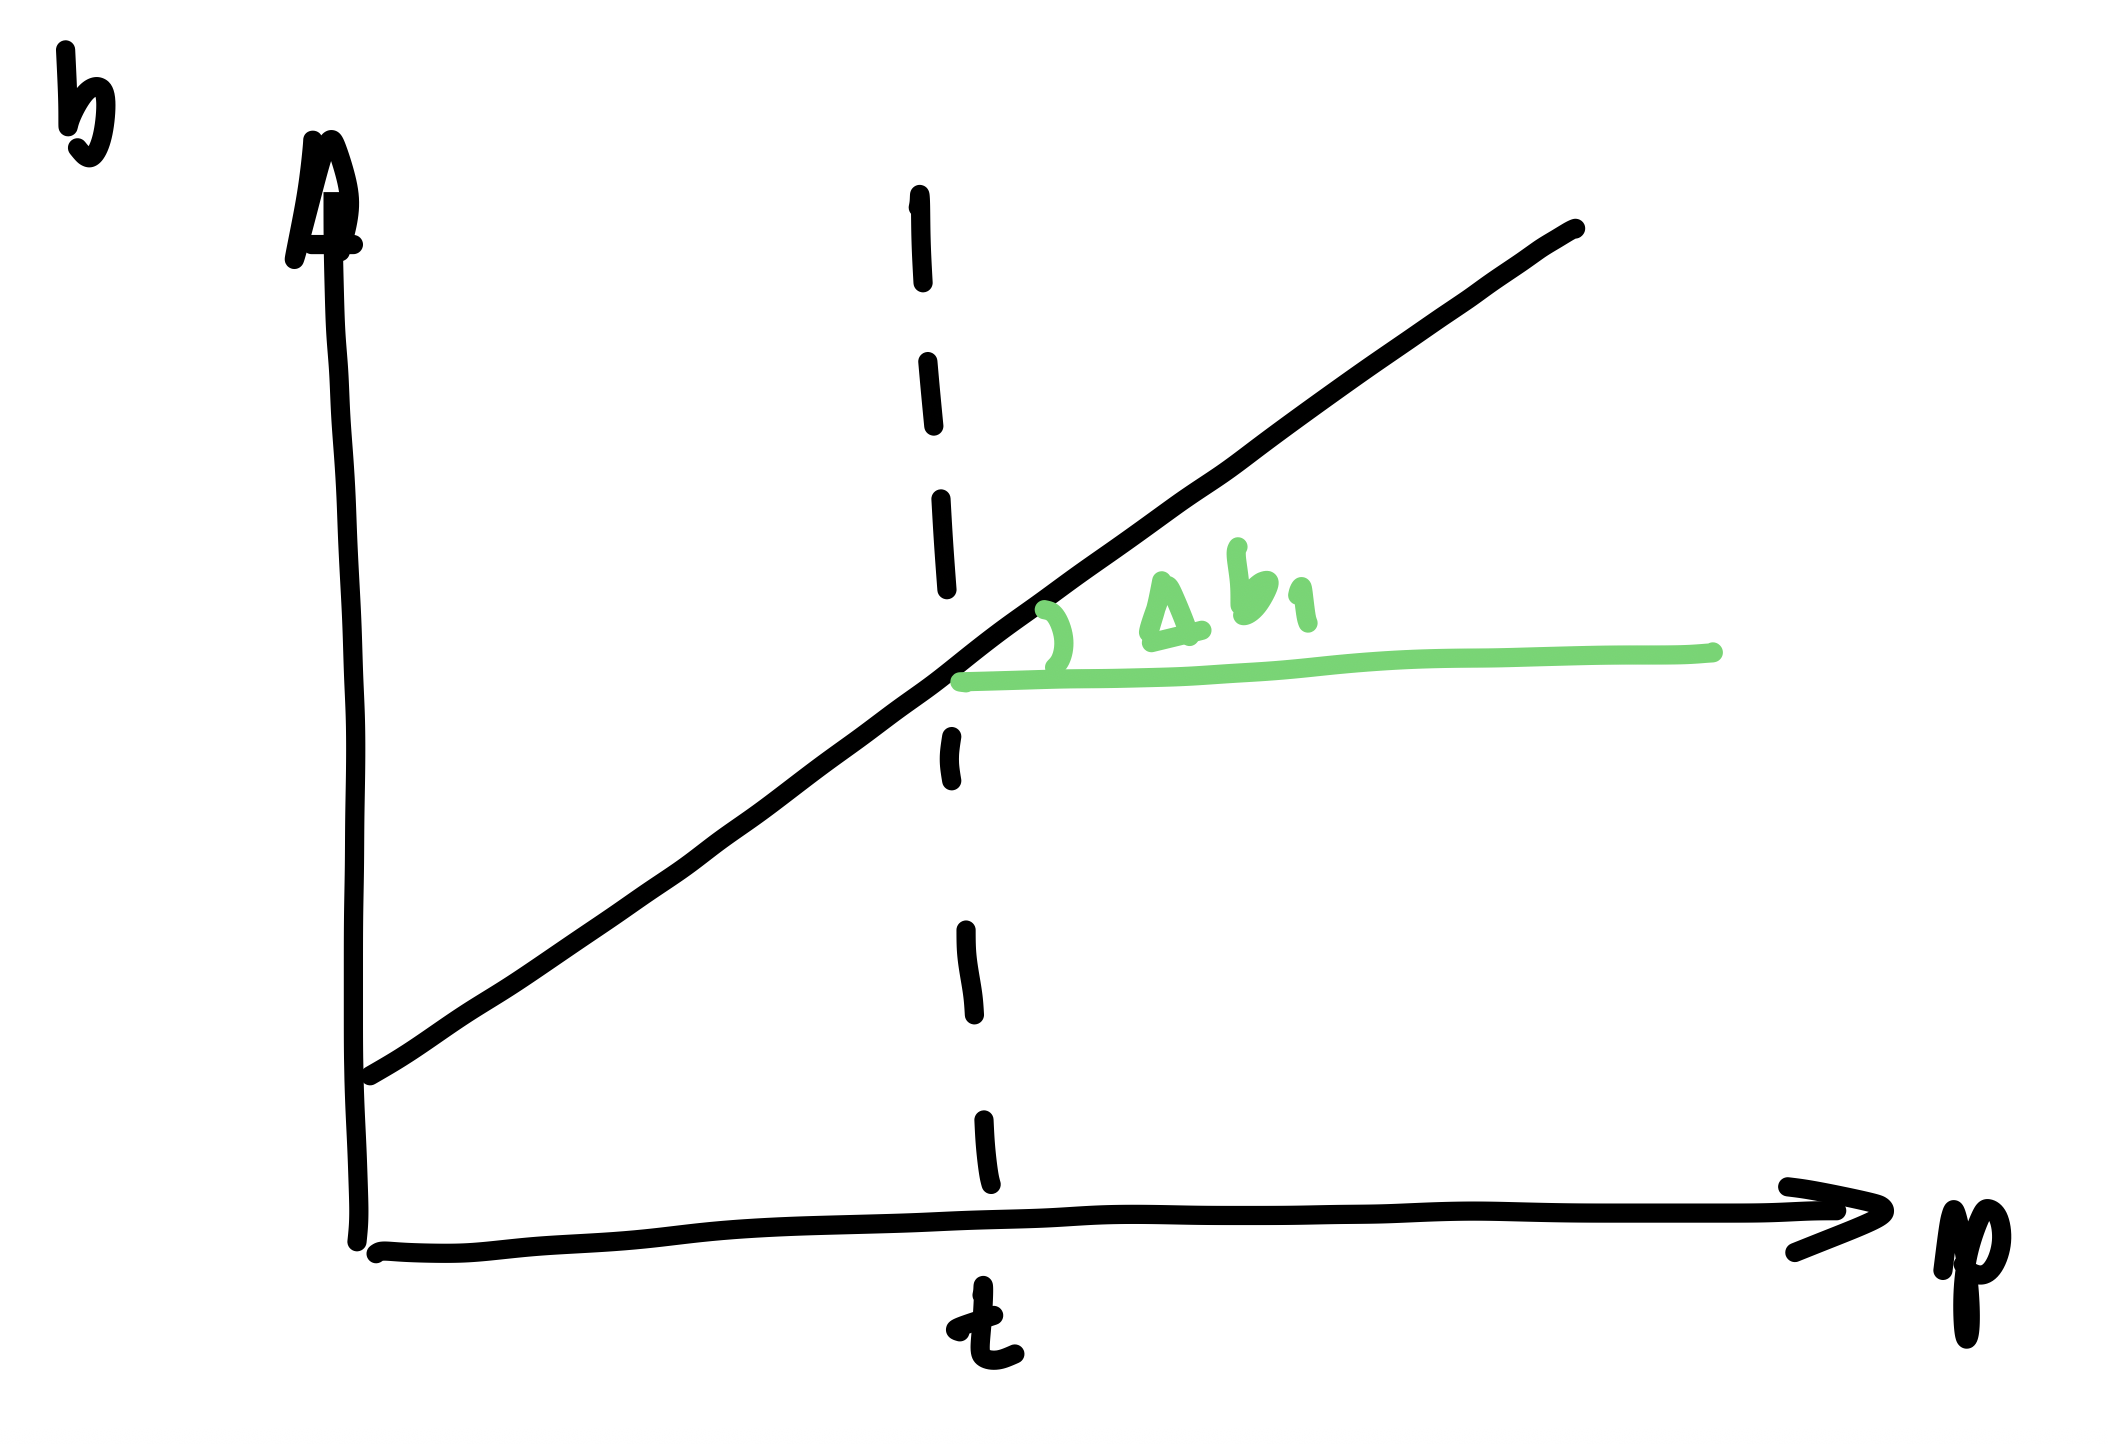
\includegraphics[width=\textwidth]{reformB1.png}
        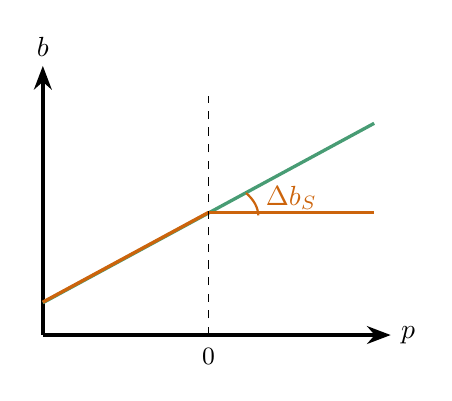
\begin{tikzpicture}
  \begin{axis}[
    width=6cm, height=5cm,
    axis lines=left,
    axis line style={-{Stealth[length=3mm]}, ultra thick},
    xmin=0, xmax=4.2, ymin=0, ymax=9,
    xtick=\empty, ytick=\empty, clip=false,
    xlabel={},
    xlabel style={at={(axis description cs:1.02,0)}, anchor=west},
    ylabel={},
  ]

    % Axis labels
    \node[anchor=south, rotate=0] at (axis description cs:0,1) {$b$};
    \node[anchor=south, rotate=0] at (axis description cs:1.05,-0.07) {$p$};

    % Black baseline line
    \addplot[very thick,col_before,domain=0:4] {1.08+1.5*x};

    % Green shifted line (parallel, upward shift)
    \addplot[very thick,col_after,domain=0:2] {1.1+1.5*x};

    % Green horizontal line
    \addplot[very thick,col_after,domain=2:4] {4.1};

    \node[col_after] at (axis cs:3,4.6) {$\Delta b_S$};

    \draw[dashed,black!60!black] (axis cs:2,0) -- (axis cs:2,8);

    % Arc to show angle
  \draw[thick,col_after] (2.6,4) arc[start angle=0,end angle=22,radius=2];

    \node at (axis cs:{2},-0.7) {\small $0$};

  \end{axis}
\end{tikzpicture}
    \end{minipage}
    
     \begin{itemize}
         \item Postergação em resposta a $\Delta b_L$ e antecipação em resposta a $\Delta b_S$
     \end{itemize}
     \bfootnote{\hyperlink{theory}{\beamerbutton{Modelo}} \hyperlink{intuition}{\beamerbutton{Intuição}}}
\end{frame}


\begin{frame}[label=counterfactualDistribution]{Distribuição Contrafactual de Requerimento}
    \centering 
    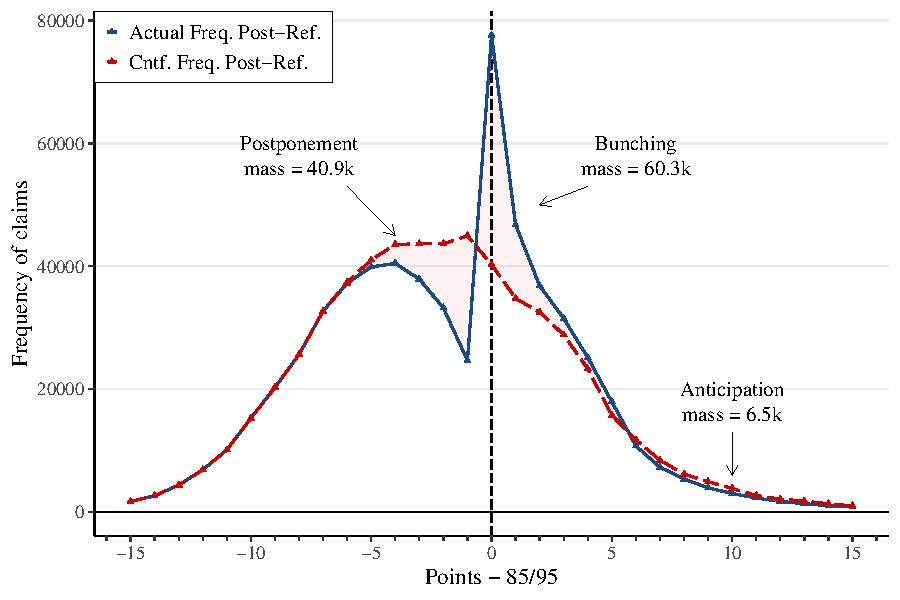
\includegraphics[width=.9\textwidth]{frequenciesAgg.pdf}
    % A little deceiving because there are individuals that claim that would not have claimed at all up to the end of 2018 (they are not in the counterfactual frequencies but are also anticipators)
\bfootnote{\hyperlink{pureLStep}{\beamerbutton{Separando Respostas}}}
\end{frame}

\begin{frame}{Conclusão}
    \begin{itemize}
        \item Documentamos respostas comportamentais grandes à reforma previdenciária de 2015
        \item Essas respostas, juntamente com o consumo relativamente mais alto dos beneficiários, geram um baixo efeito de bem-estar por real gasto
        \begin{itemize}
            \item WMVPF = 0.26 e MVPF = 0.32
        \end{itemize}
        \item O efeito de bem-estar por real é maior para $b_S$ do que para $b_L$, o que implica que a reforma ótima neutra em orçamento deveria
        \begin{itemize}
            \item Aumentar a inclinação do benefício
            \item Reduzir o nível do benefício
        \end{itemize}
        % \item If the government wants to spend optimally closing the budget with payroll taxes, it should increase the slope
    \end{itemize}
\end{frame}
%-----------------------------------------------------------

\begin{frame}
    \begin{itemize}
        \item Thank you!
        \begin{itemize}
            \item gtlemos@mit.edu
            \item juanrios@econ.puc-rio.br
            \item gonzaga@puc-rio.econ.br
            
            
        \end{itemize}
    \end{itemize}
\end{frame}

\appendix


\begin{frame}[label=literature]{Literatura Relacionada}
\begin{enumerate}
    \item \textbf{Efeitos de reformas previdenciárias}
    \vspace{0.3em}

    \begin{itemize}
        \item Friedberg (2000), Manoli \& Weber (2016), Seibold (2021), Lalive et al (2023),  Giupponi (2025)
        \vspace{0.3em}
        \item[\textcolor{violet}{$\rightarrow$}] \textcolor{violet}{A reforma permite separar respostas a nível e inclinação}
        
    \end{itemize}
    
    \vspace{0.3em}
    
    \item \textbf{Análise de bem-estar e desenho ótimo da previdência}
    \vspace{0.3em}
    
    \begin{itemize}
         \item Huggett e Parra (2010), Hosseini and Shourideh (2019), Giesecke and Jager (2021), Haller (2022), Kolsrud et al (2024), Seibold and Reck (2025), McKiernan (2022), Ndiaye and Yu (2025), 
        \item[\textcolor{violet}{$\rightarrow$}] \textcolor{violet}{Separar o efeito de bem-estar de diferentes parâmetros e orientar a reforma ótima com base em estatísticas suficientes}
    \end{itemize}
    \item \textbf{Estatísticas suficientes p/ análise de bem-estar e políticas ótimas}
    \vspace{0.3em}
    \begin{itemize}
        \item Feldstein (1999), Chetty (2009), Kleven (2018), Hendren and Sprung-Keyser (2020), Bergstrom et al (2026)
        \item[\textcolor{violet}{$\rightarrow$}] \textcolor{violet}{Arcabouço de estatísticas suficientes para reforma ótima local}
    \end{itemize}
\end{enumerate}
\bfootnote{\hyperlink{mainResults}{\beamerbutton{back}}}
\end{frame}

\begin{frame}[label=dataReplacement]{Distribuição Empírica}
          \centering
          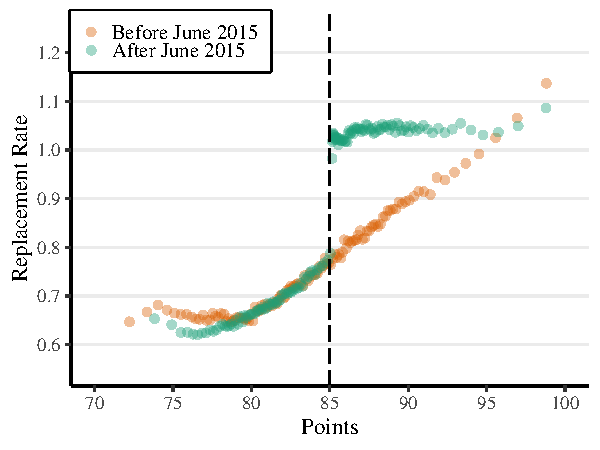
\includegraphics[width=.8\linewidth]{E4_pension_schedule_women.pdf}
    \bfootnote{\hyperlink{reform}{\beamerbutton{Voltar}}}
\end{frame}

\begin{frame}[label=men]{Taxa de Reposição dos Homens}
    \begin{columns}
        \begin{column}{0.45\textwidth}
            \centering
            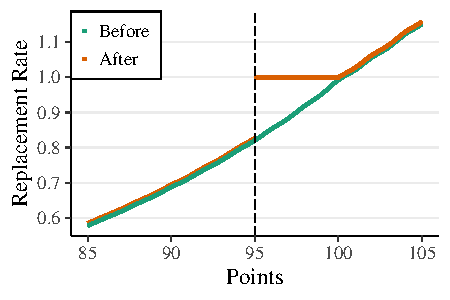
\includegraphics[width=\linewidth]{schedule_men_new.pdf}
        \end{column}
        \begin{column}{0.45\textwidth}
          \centering
          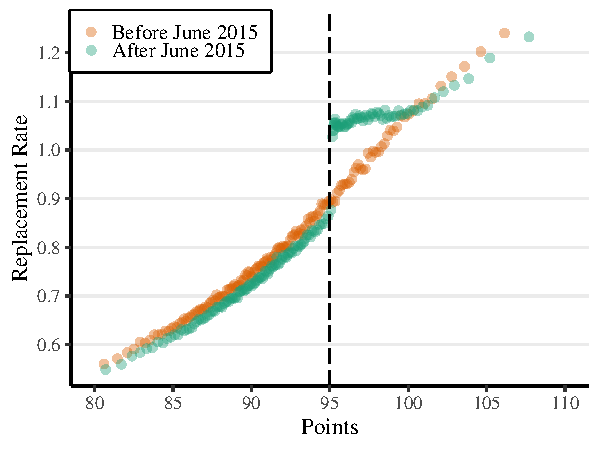
\includegraphics[width=\linewidth]{E4_pension_schedule_men.pdf}
        \end{column}
    \end{columns}
    \bfootnote{\hyperlink{reform}{\beamerbutton{Voltar}}}
\end{frame}

\begin{frame}[label=rfEvidenceWomen]{Evidência em Forma Reduzida (Mulheres)}
    \centering
    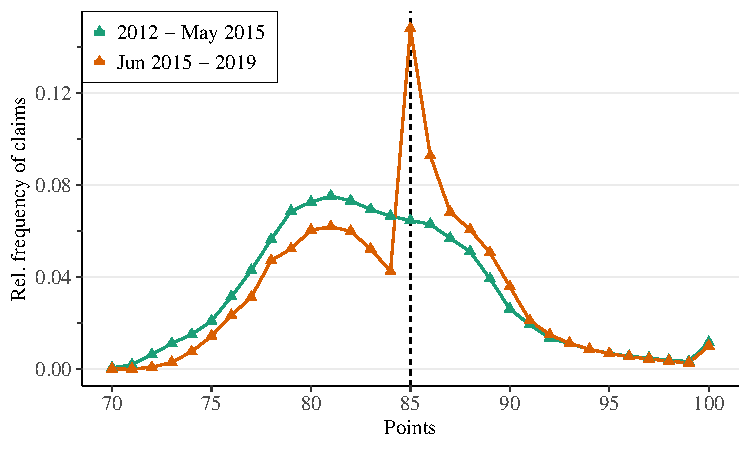
\includegraphics[width=.9\linewidth]{E3_claiming_density_women.pdf}
    \bfootnote{\hyperlink{rfEvidence}{\beamerbutton{Voltar}}}
\end{frame}

\begin{frame}[label=rfEvidenceMen]{Evidência em Forma Reduzida (Homens)}
    \centering
    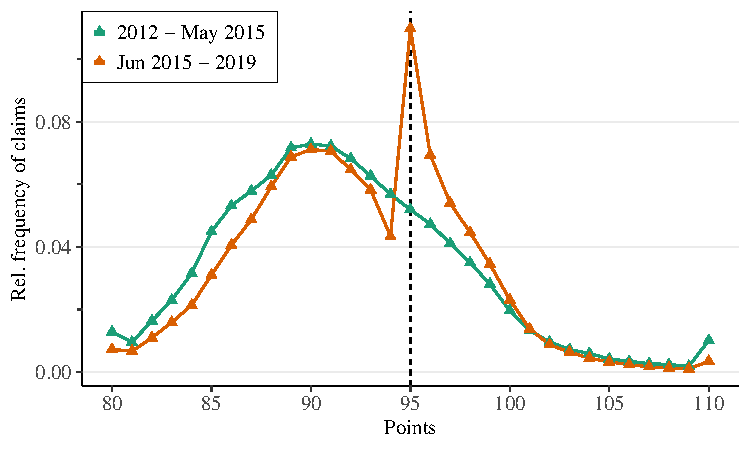
\includegraphics[width=.9\linewidth]{E3_claiming_density_men.pdf}
    \bfootnote{\hyperlink{rfEvidence}{\beamerbutton{Voltar}}}
\end{frame}



\begin{frame}[label=chDdOther]{Efeito Negativo sobre o CH em $p\in [-6,-2)$}
    \centering
    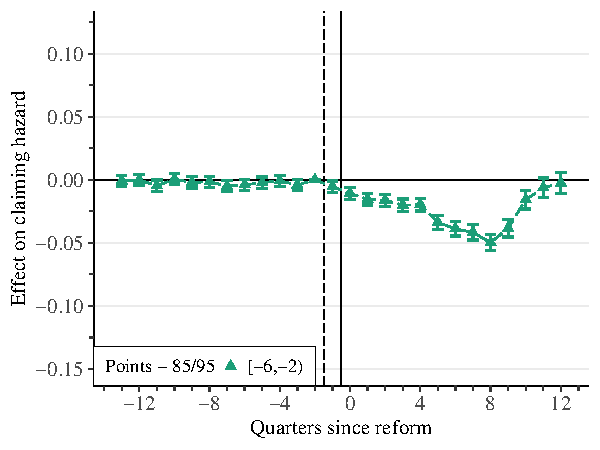
\includegraphics[width=0.7\linewidth]{F4_eventstudy_agg_1.pdf}
\end{frame}

\begin{frame}{Efeito Positivo de Curto Prazo sobre os CHs em $p\in [2,6]$}
    \centering
    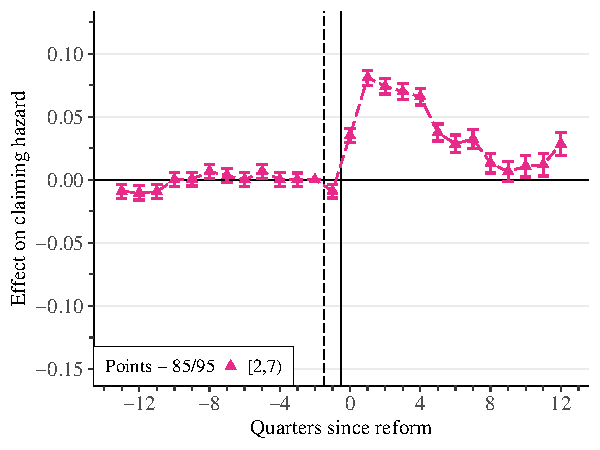
\includegraphics[width=0.7\linewidth]{F4_eventstudy_agg_4.pdf}
\end{frame}

\begin{frame}{Efeito Positivo de Curto Prazo sobre os CHs em $p\in [7,\bar 15]$}
    \centering
    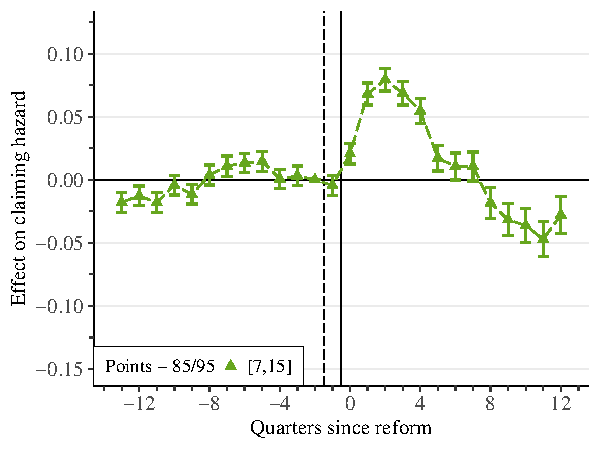
\includegraphics[width=0.7\linewidth]{F4_eventstudy_agg_5.pdf}
    \bfootnote{\hyperlink{ChDdRightAbove}{\beamerbutton{Voltar}}}
\end{frame}

\begin{frame}[label=trend]{CH para Todas as Faixas de Pontos}
    \centering
    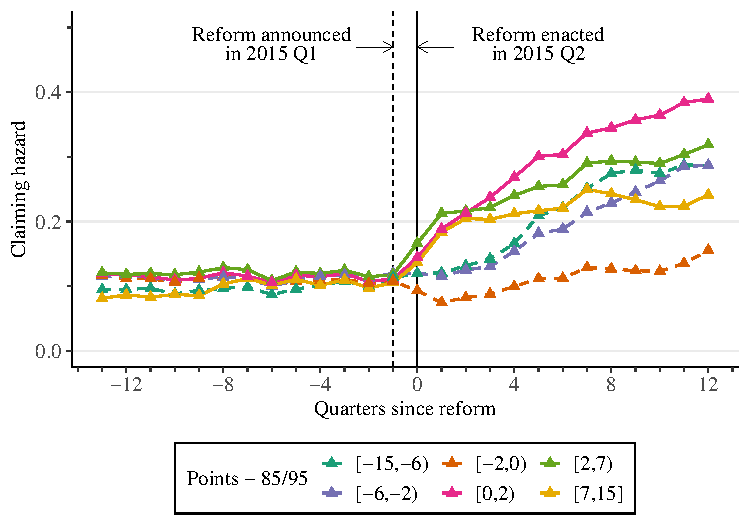
\includegraphics[width=.9\linewidth]{E3_claiming_haz_quarters_group.pdf}
    \bfootnote{\hyperlink{ChDdRightAbove}{\beamerbutton{Voltar}}}
\end{frame}

\begin{frame}[label=selectionOther]{Efeito sobre os Benefícios Médios Pré-Reforma em $p \in [\bar p-6,\bar p-2)$}
    \centering
    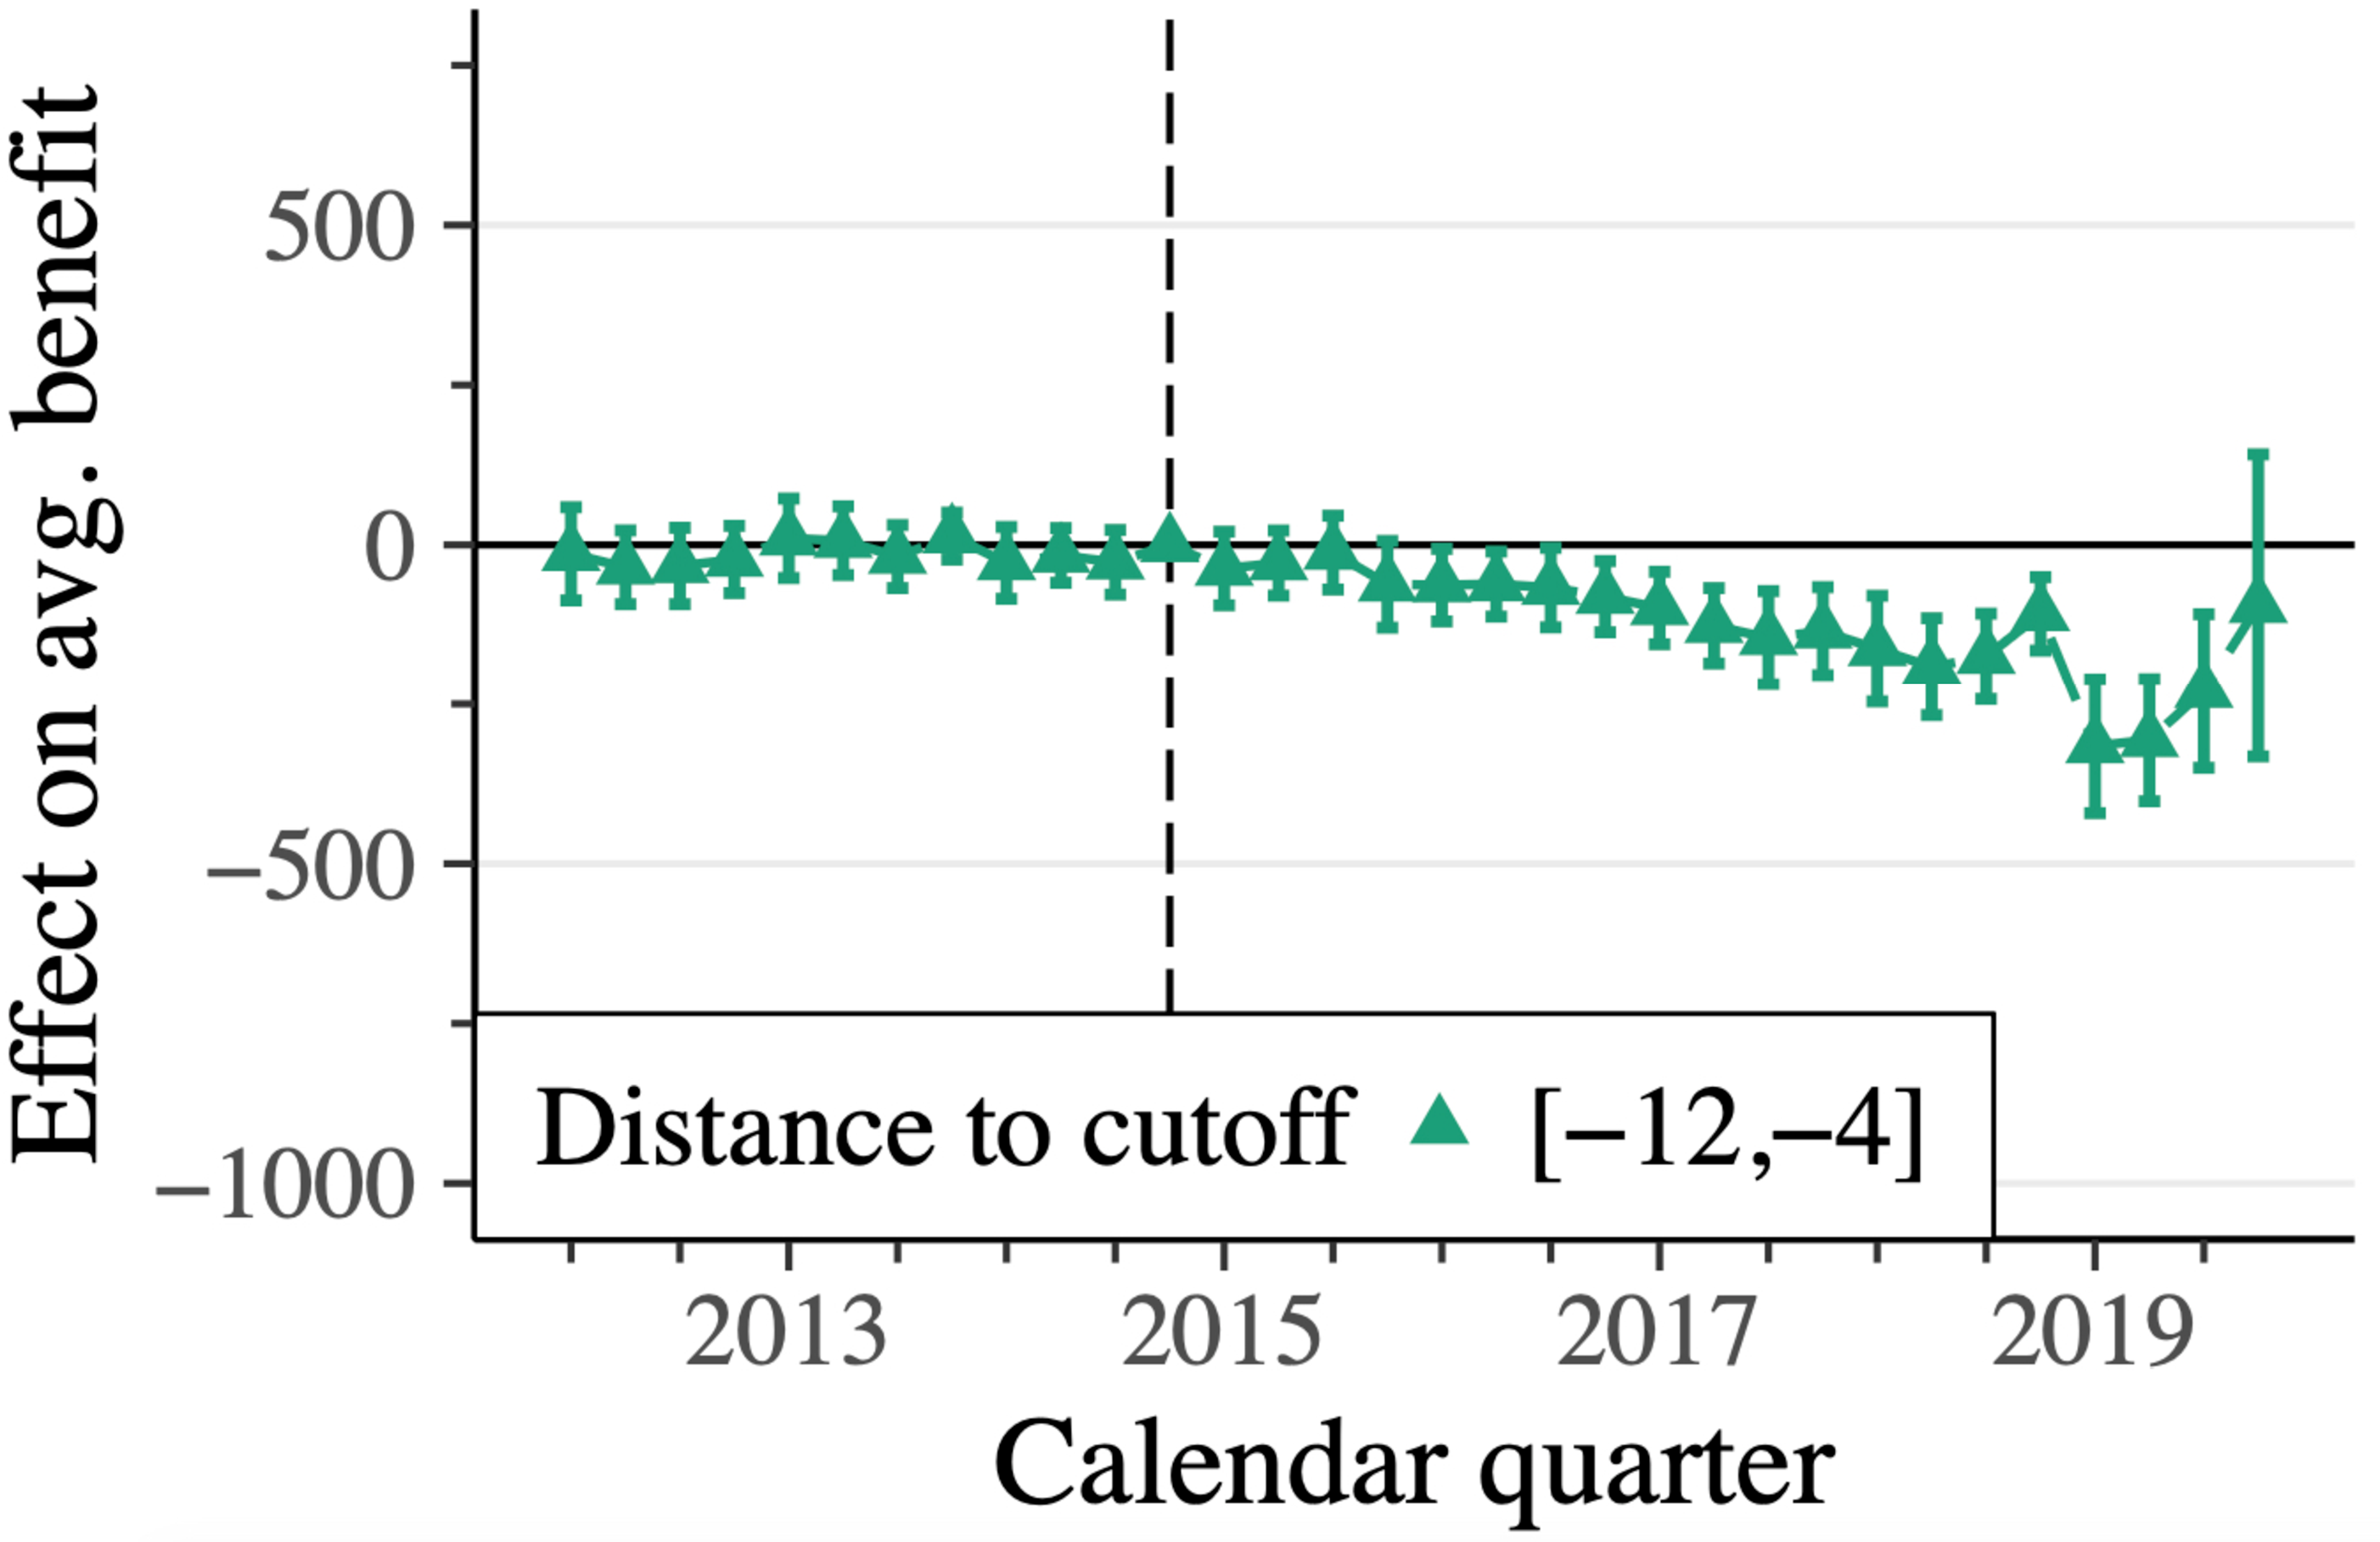
\includegraphics[width=0.8\linewidth]{old-12.pdf}
\end{frame}

\begin{frame}{Efeito sobre os Benefícios Médios Pré-Reforma em $p \in [\bar p+2,\bar p+6)$}
    \centering
    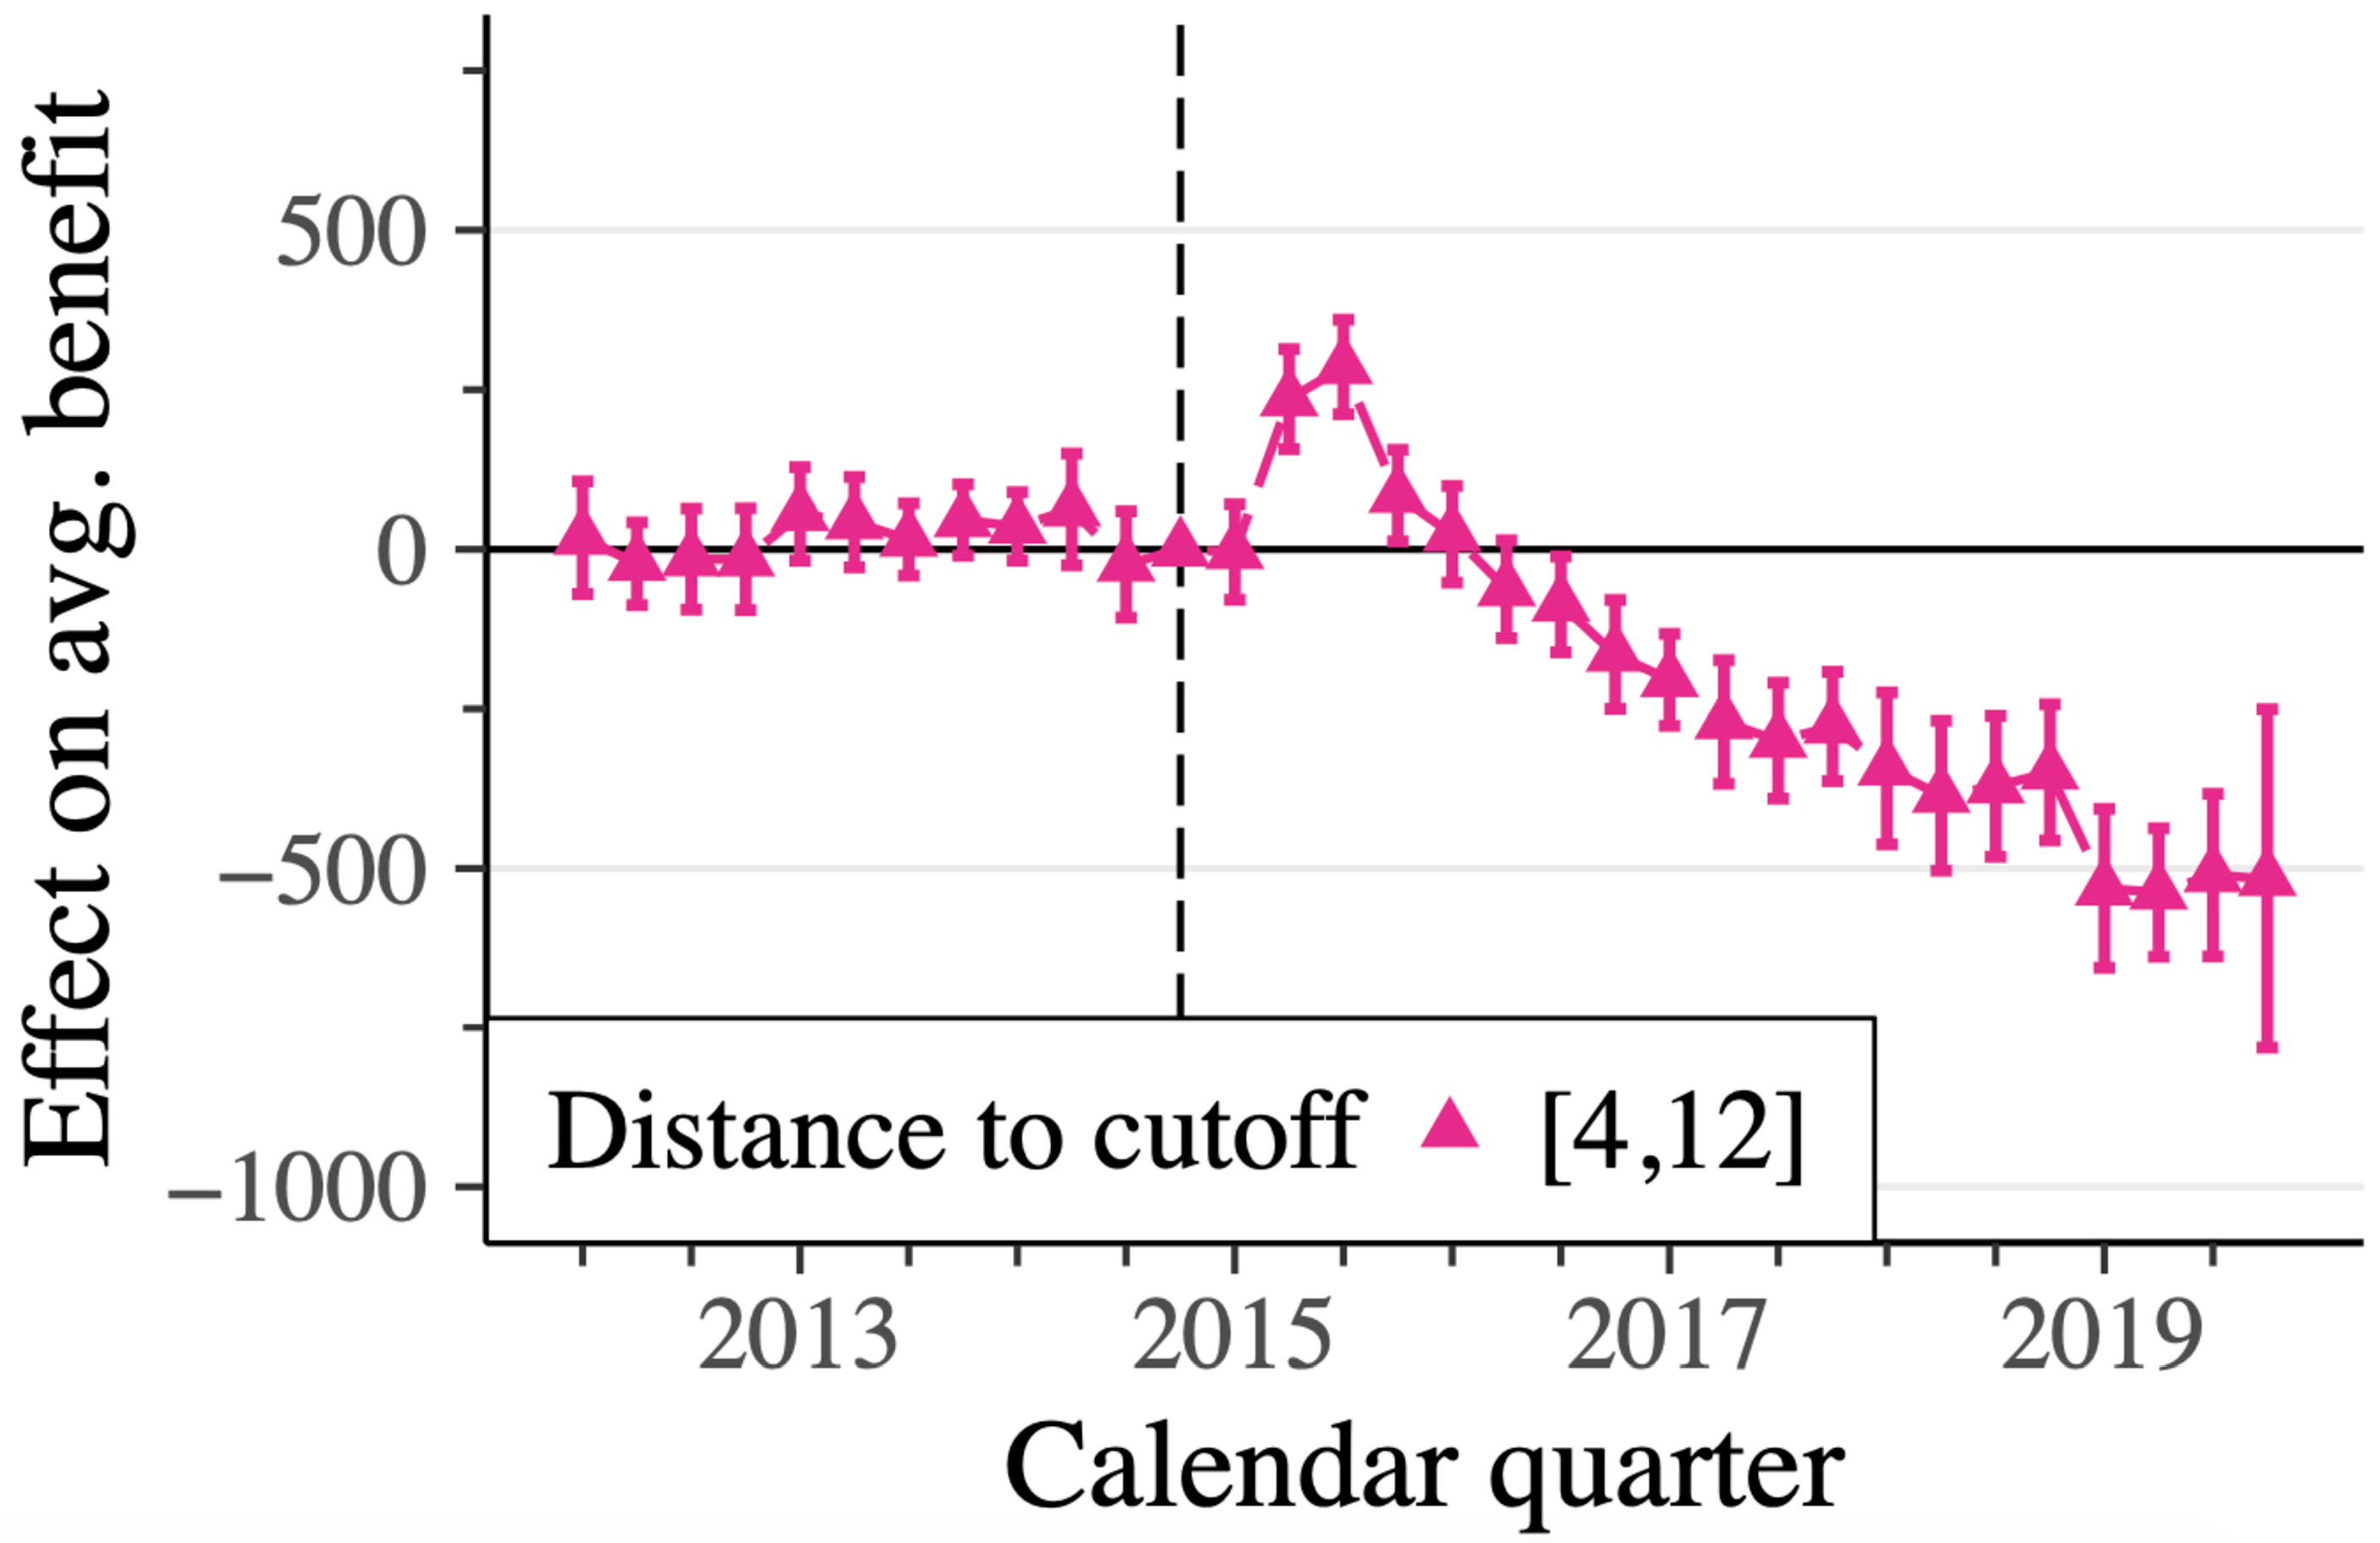
\includegraphics[width=0.8\linewidth]{old4.pdf}
\end{frame}

\begin{frame}{Efeito sobre os Benefícios Médios Pré-Reforma em $p \in [\bar p+6,\bar p+15]$}
    \centering
    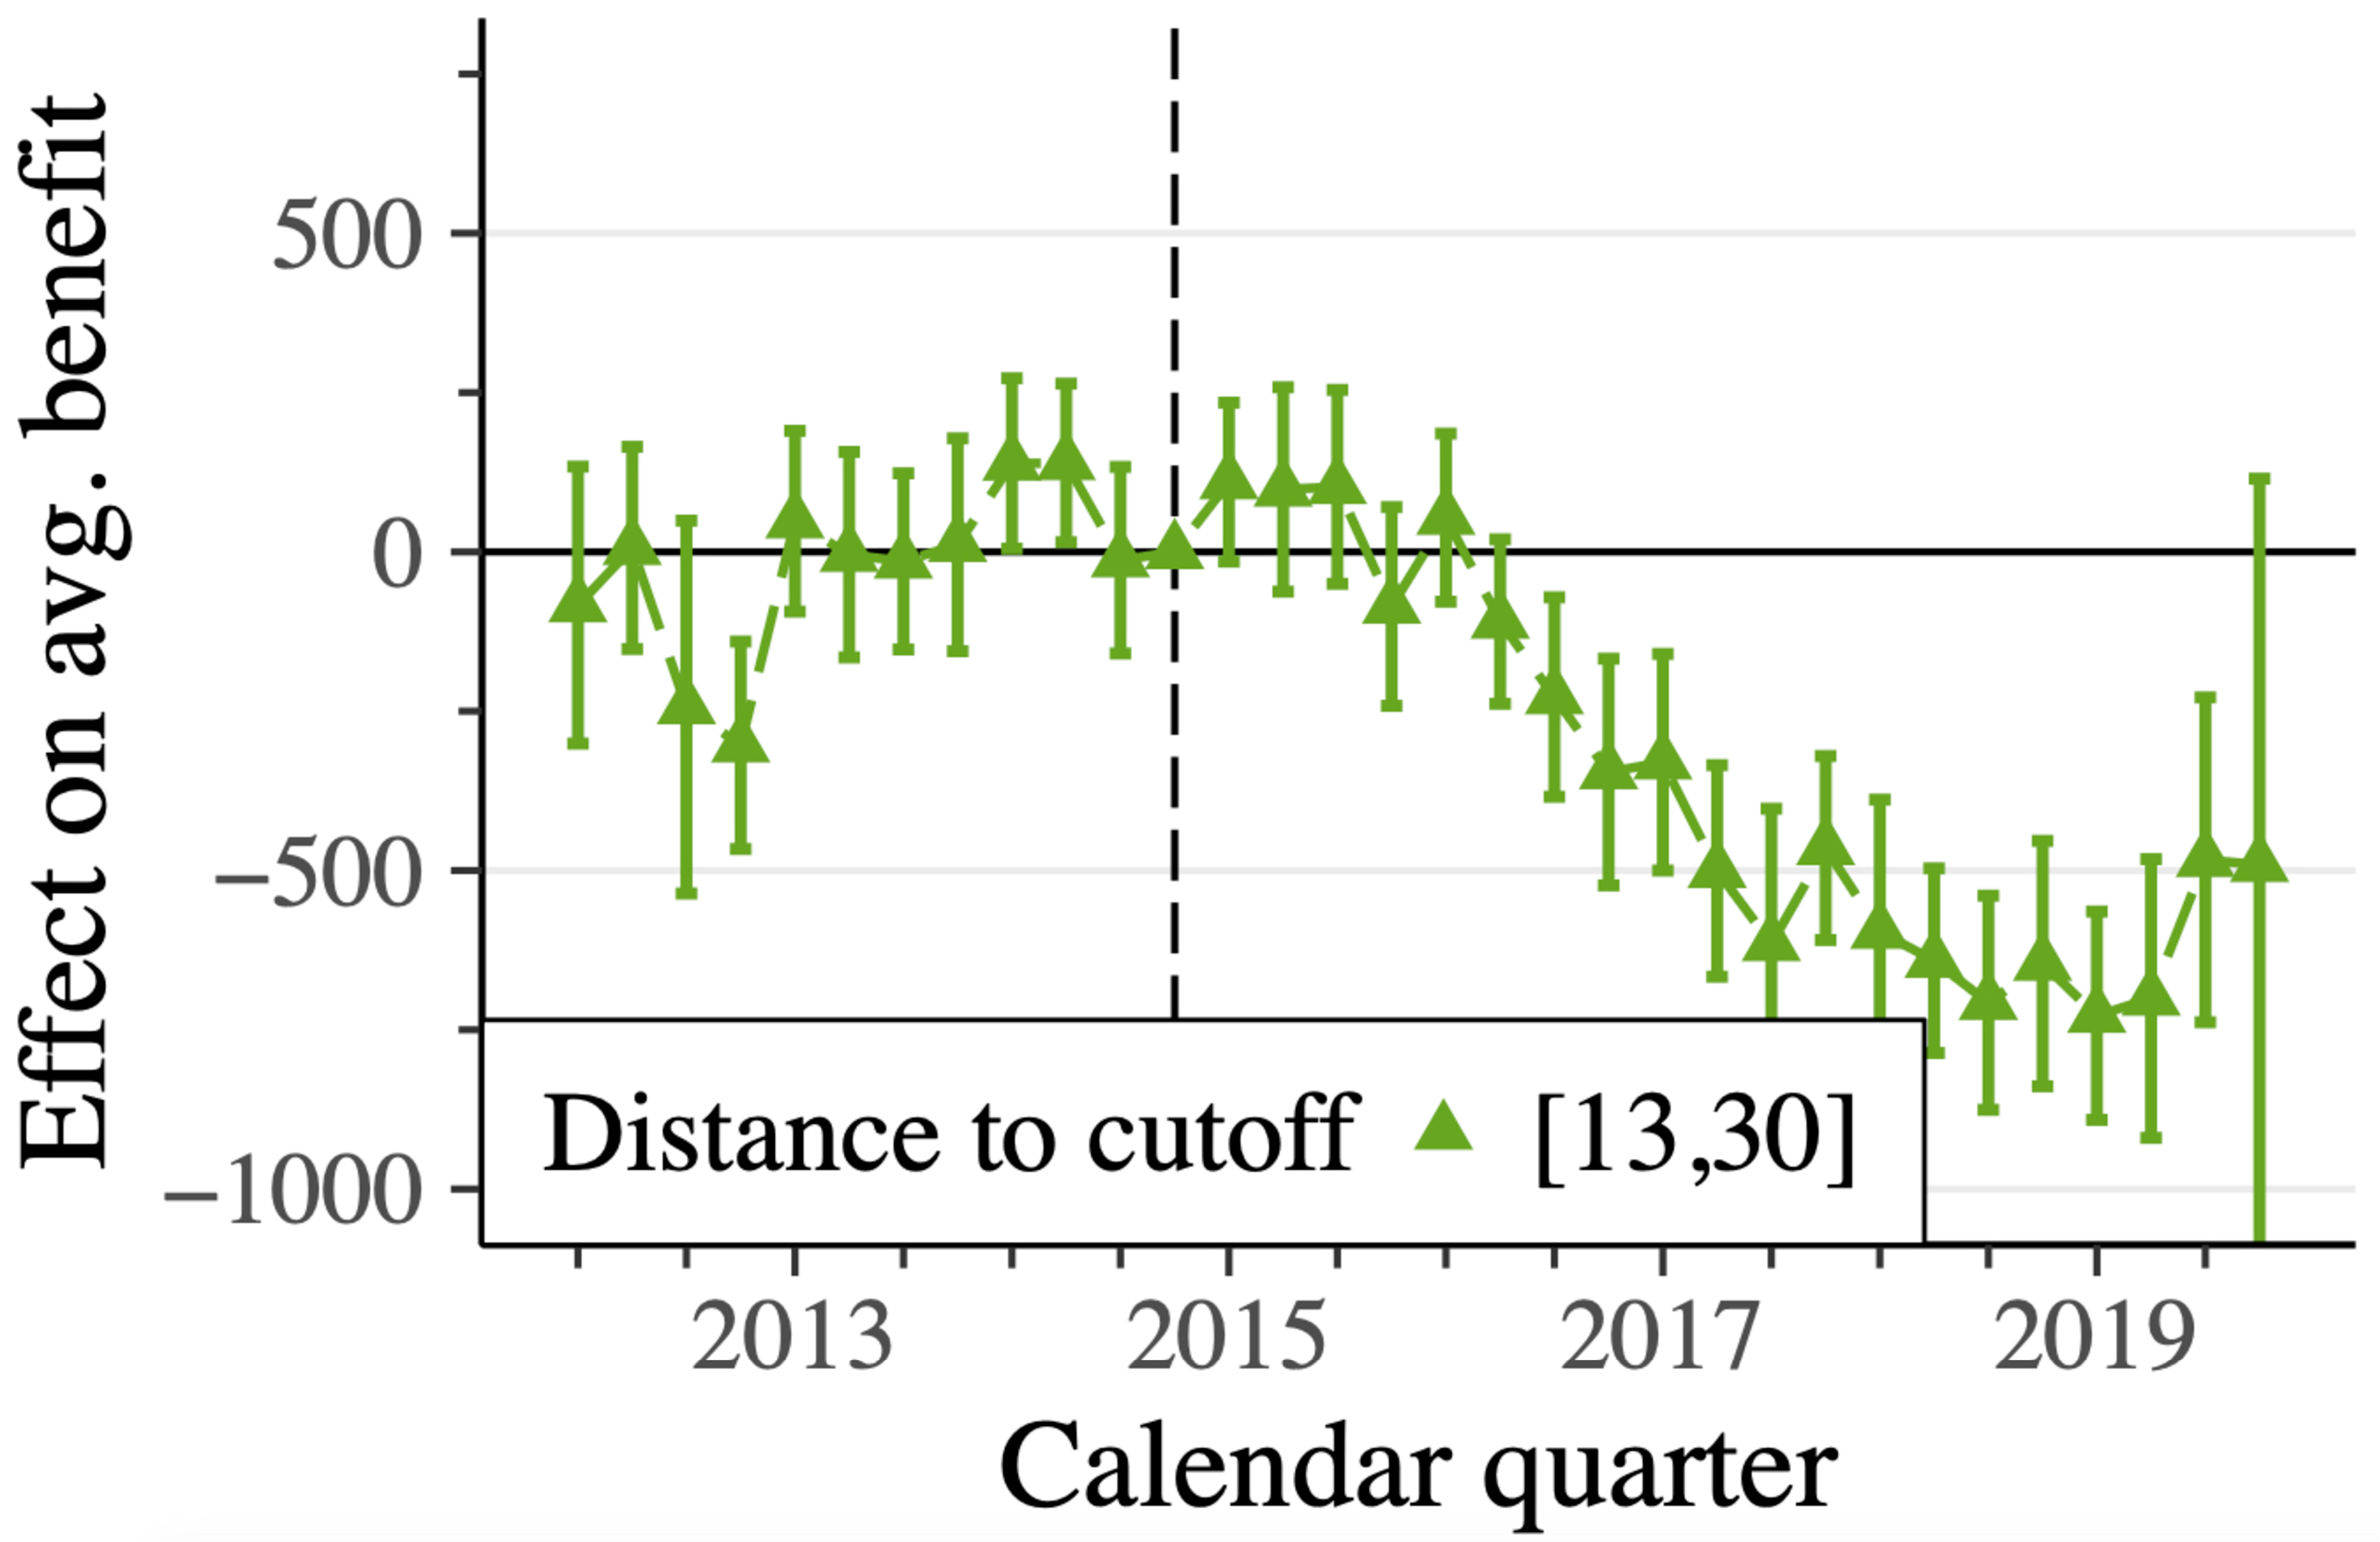
\includegraphics[width=0.8\linewidth]{old13.pdf}
    \bfootnote{\hyperlink{selectionRightAbove}{\beamerbutton{Voltar}}}
\end{frame}

\begin{frame}[label=chToFrequencies]{Recuperando Frequências Contrafactuais a partir dos Hazards de Requerimento}
    \begin{itemize}
        \item Seja $C_{pt}$ o número de requerimentos e $R_{pt}$ o número de requerentes potenciais em $(p,t)$, de modo que $CH_{pt}=C_{pt}/R_{pt}$
        \item Antes do anúncio: $C^c_{p,-2}=C_{p,-2}$ e $R^c_{p,-2}=R_{p,-2}$
        \begin{block}{Hipótese 1: Acumulação Determinística de Pontos}
            Os pontos normalizados aumentam deterministicamente em $\Delta p= 0.5$, correspondendo a contribuições contínuas no emprego formal até o requerimento.
        \end{block}
        \item Requerentes potenciais em $t+1$ = sobreviventes de $t$ + entradas em $t+1$
        \[
        R_{p+\Delta p,\,t+1}^c = R_{pt}^c - C_{pt}^c + I_{p+\Delta p,\,t+1}
        = R_{pt}^c \left(1 - CH_{pt}^c\right) + I_{p+\Delta p,\,t+1},
        \]
        \item $I_{pt}$: número de trabalhadores que se tornam elegíveis com $p$ pontos em $t$
        \item A frequência contrafactual é recuperada usando $C_{pt}^c = R^c_{pt} CH^c_{pt}$
    \end{itemize}
    \bfootnote{\hyperlink{ChDdRightAbove}{\beamerbutton{Voltar}}}
\end{frame}

\begin{frame}[label=npv]{Valor Presente dos Benefícios Líquidos de Impostos}
    \begin{itemize}
        \item Podemos medir $\sum_{t=0}^{T} \frac{b^a(x_{it}^a)}{(1+r)^t}$ e $\sum_{t=0}^{T}  \frac{\tau(x_{it}^a)}{(1+r)^t}$
        \begin{itemize}
            \item Onde $T$ é o último trimestre dos nossos dados
        \end{itemize}
        \item Precisamos obter $b_i^{PDV}\equiv  \sum_{t=0}^{T_i} \frac{b^a(x_{it}^a)}{(1+r)^t}$ e $\tau_i^{PDV}\equiv  \sum_{t=0}^{T_i}  \frac{\tau(x_{it}^a)}{(1+r)^t}$
        \begin{itemize}
            \item Onde $T_i$ é o número de trimestres até a morte de $i$, mas $T_i>T$
        \end{itemize}
        \item Medimos $T_i$ assumindo que os indivíduos vivem até a expectativa de vida condicional à sua idade e sexo
        \item Como os benefícios mensais são constantes, podemos estimar $b_i^{PDV}$
        \item Em andamento: estimar $\tau_i^{PDV}$ usando Surrogate Index (Athey et al, 2025)
    \end{itemize}
    \bfootnote{\hyperlink{npvTaxes}{\beamerbutton{Surrogate Index}}}
\end{frame}

\begin{frame}[label=npvTaxes]{Estimando o VPD da Arrecadação Tributária}
    \begin{itemize}
        \item Estimamos $\tau_i^{PDV}$ usando Surrogate Index (Athey et al, 2025)
        \begin{enumerate}
            \item Usando a amostra de trabalhadores de 1995-2000, podemos computar $\tau^{PDV}_{i}$ assumindo que eles param de trabalhar em até 20 anos
            \item Prever $\tau^{PDV}_{i}$ com observáveis (renda, setor, idade etc.)
            \item Usar (2) para prever $\tau_i^{PDV}$ para aqueles na nossa amostra (2012-2018)
        \end{enumerate}
    \end{itemize}
    \bfootnote{\hyperlink{empiricalOverviewDAP}{\beamerbutton{Voltar}}}
\end{frame}

\begin{frame}[label=tax]{Efeito sobre a Arrecadação Tributária}
    \begin{itemize}
        \item Exploramos o fato de que trabalhadores com rendimentos $<$ 1.25 vezes o salário mínimo não foram afetados pela reforma, pois os benefícios são limitados ao salário mínimo
         \begin{align*}
            \label{eq_dd_taxes}
            \Delta \tau_{i,t} = \delta_i^{tax}+\gamma_t^{tax} + \sum_{k\neq -2}\beta_k^{tax}1(w_{it}>1.25MW) \times 1(t = k) +\varepsilon^{tax}_{it}
        \end{align*}
        \begin{assumption}[Crescimento Paralelo]
            \label{ass_parallelTaxes}
             Se a reforma não tivesse ocorrido, a mudança na arrecadação tributária dos trabalhadores com salários de contribuição abaixo de 1.25 salários mínimos teria permanecido paralela à mudança observada para aqueles acima desse valor.
        \end{assumption}
        \item Restrito a trabalhadores com até 5 salários mínimos ($\approx 80$\%)
    \end{itemize}
\end{frame}

\begin{frame}{Resultados de Arrecadação Tributária (DD)}
    \centering
    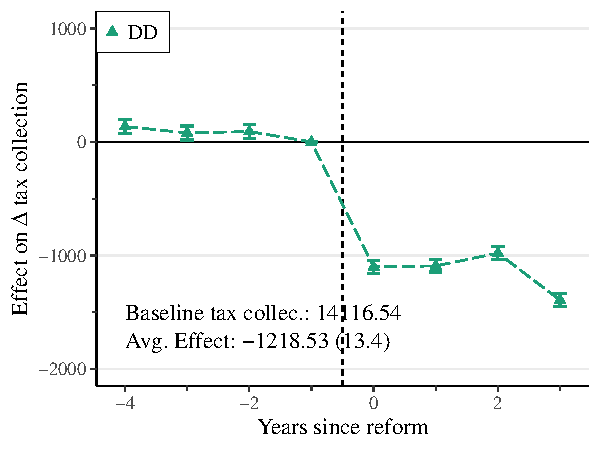
\includegraphics[width=0.7\linewidth]{H2_dd_tax_collection_1.pdf}
    \bfootnote{\hyperlink{MEandFE}{\beamerbutton{Voltar}}}
\end{frame}

\begin{frame}[label=mechanicalOther]{Efeito sobre os Benefícios Médios Pós-Reforma em $p \in [\bar p-6,\bar p-2)$}
    \centering
    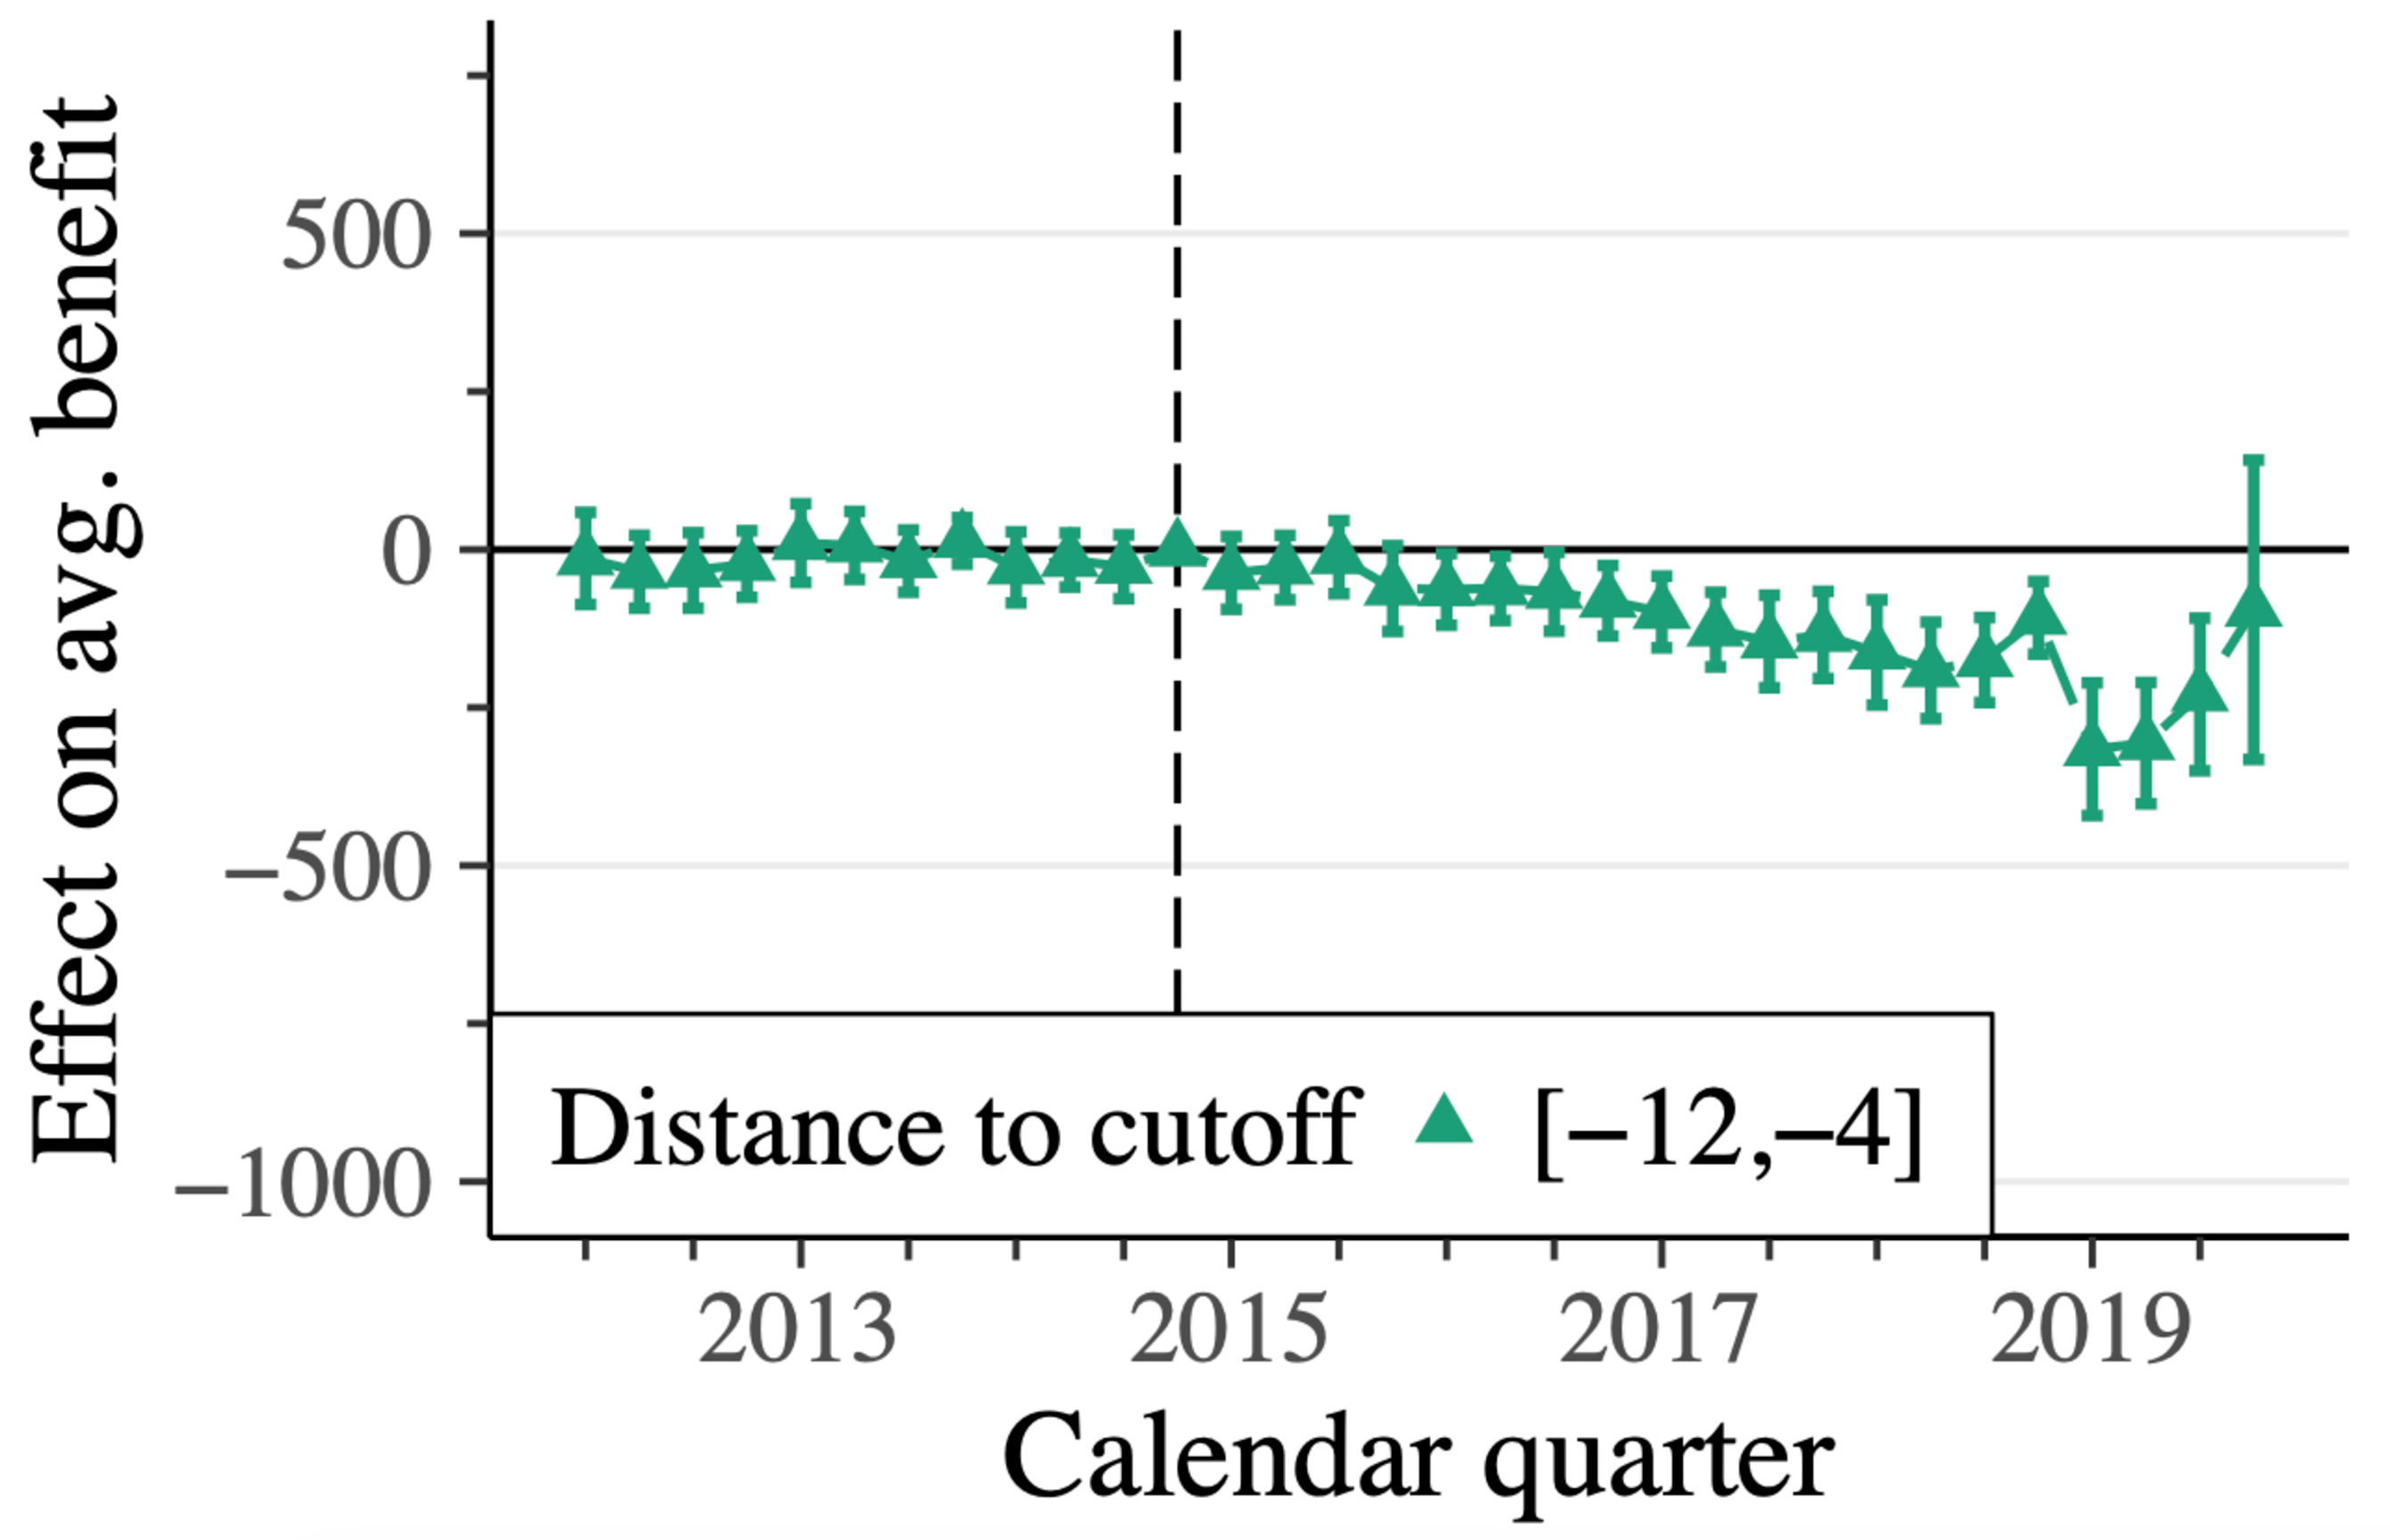
\includegraphics[width=0.8\linewidth]{new-12.pdf}
\end{frame}

\begin{frame}{Efeito sobre os Benefícios Médios Pós-Reforma em $p \in [\bar p+2,\bar p+6)$}
    \centering
    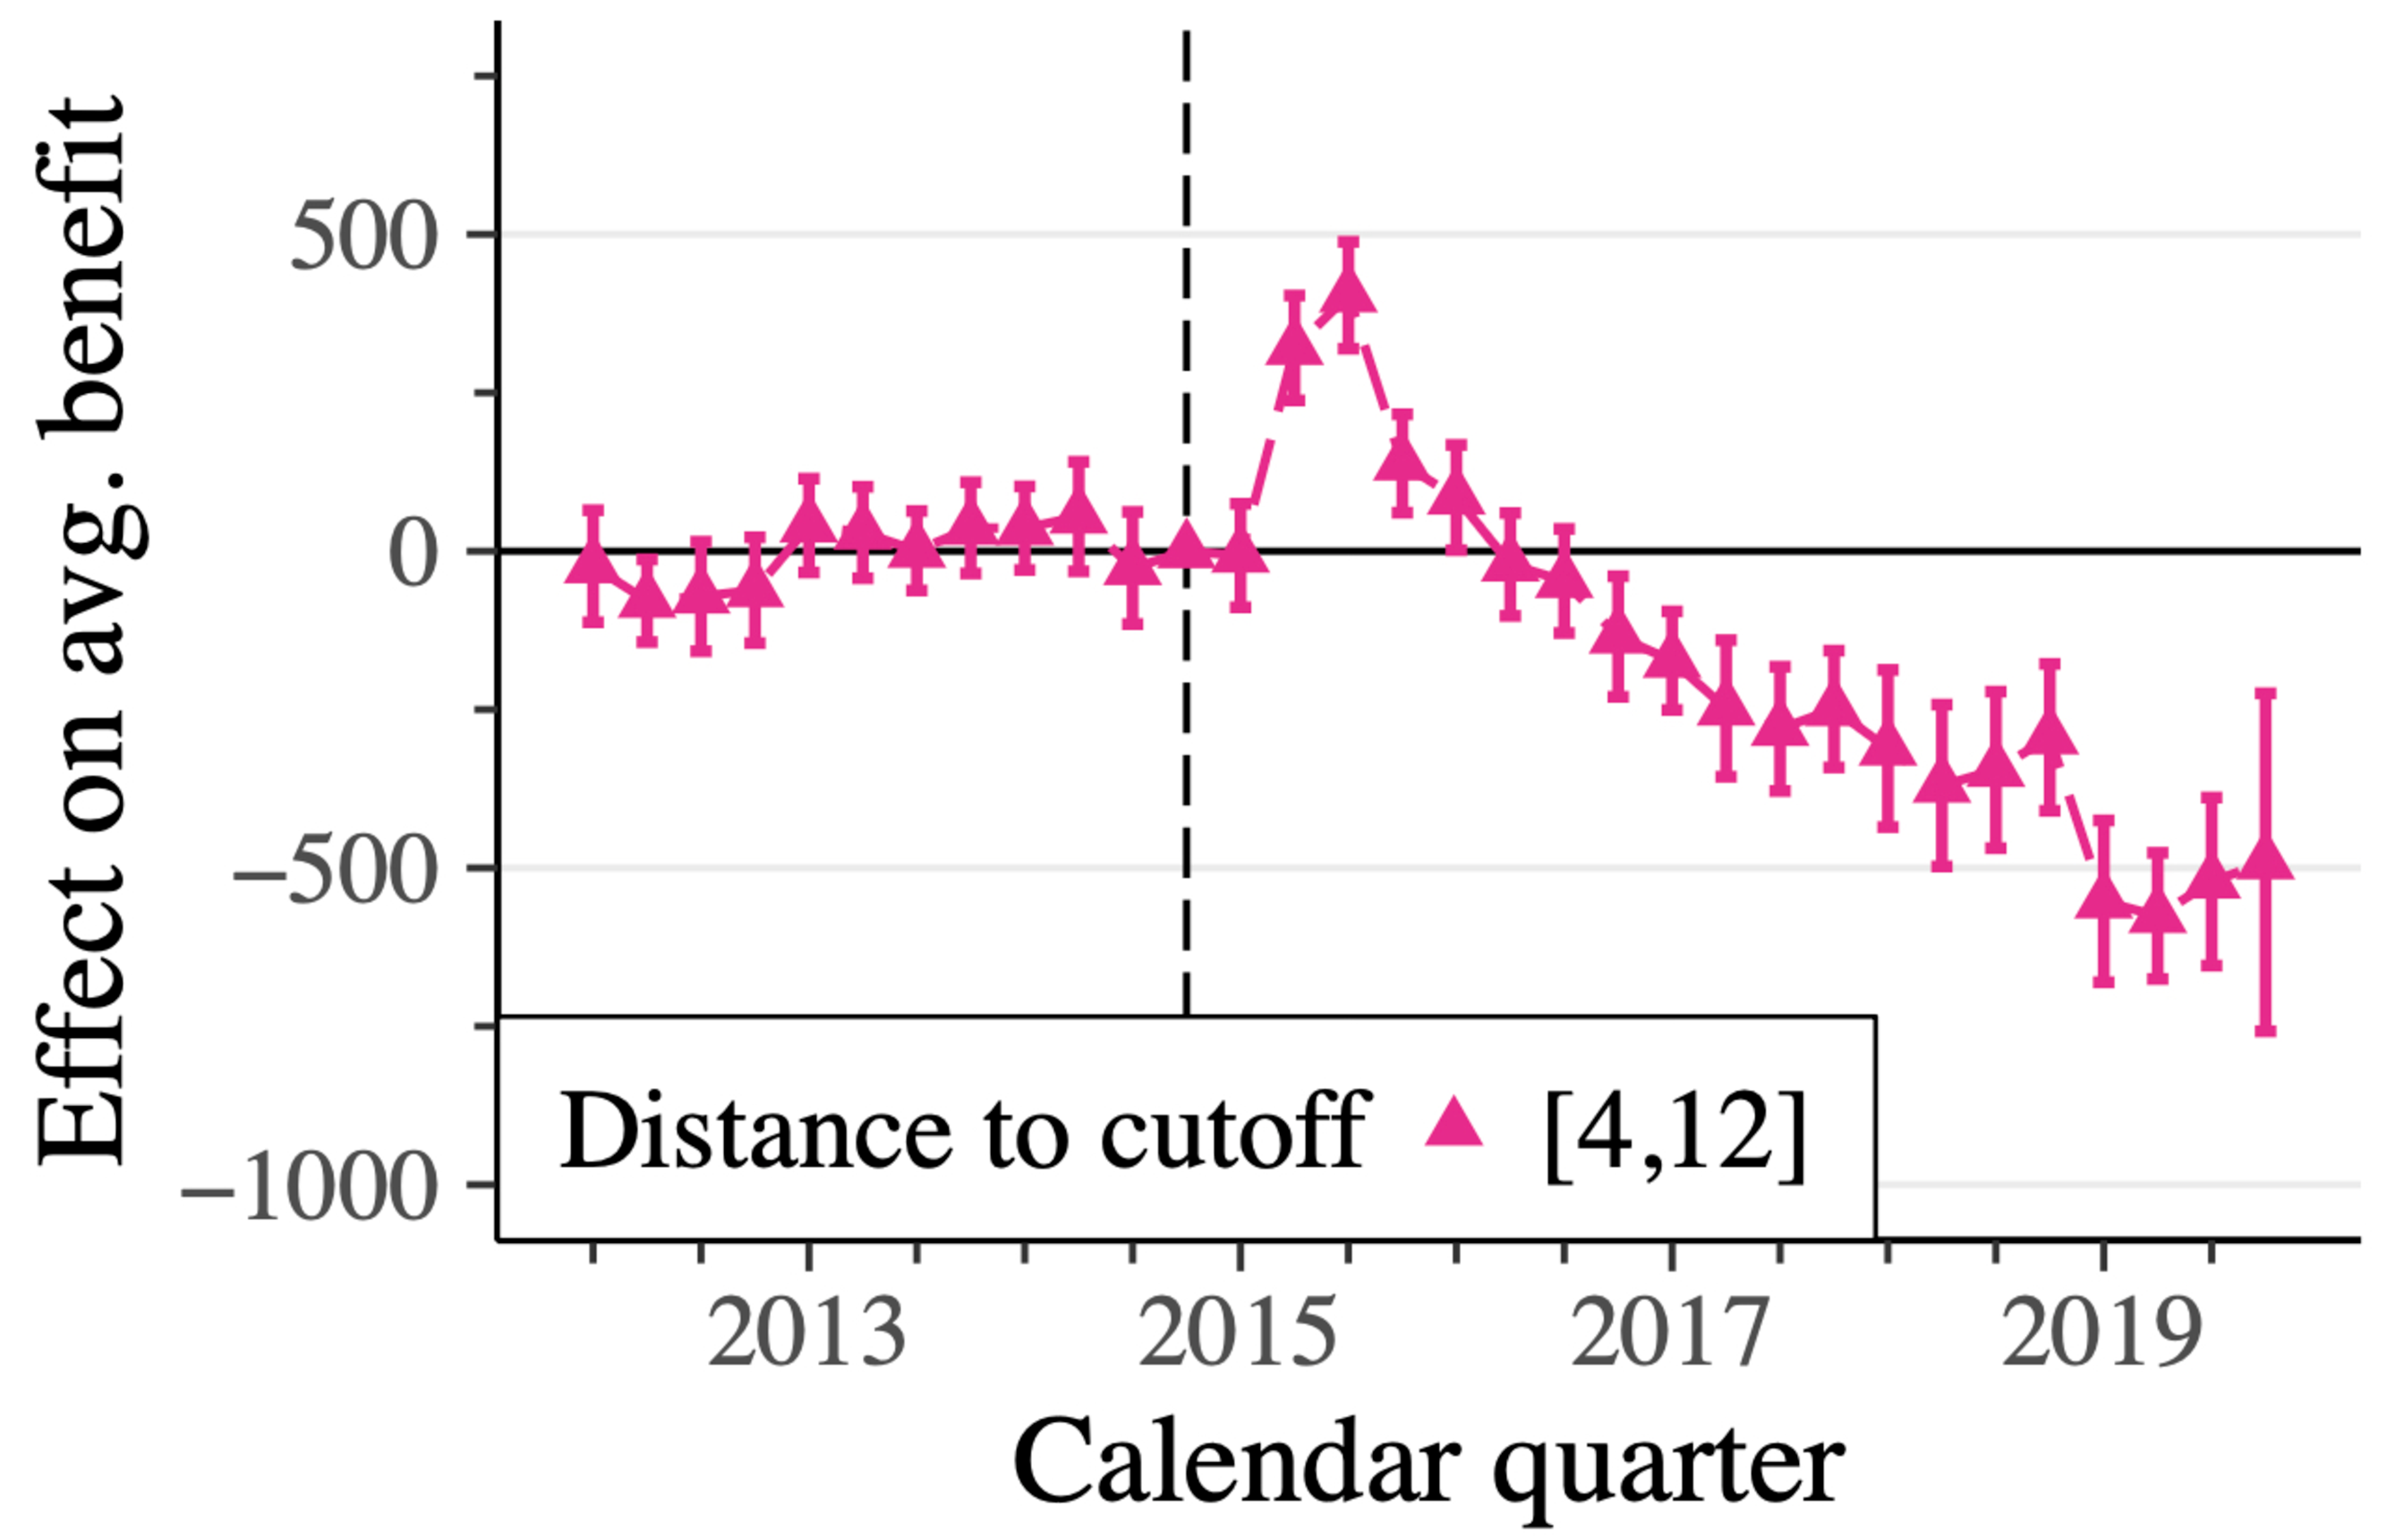
\includegraphics[width=0.8\linewidth]{new4.pdf}
\end{frame}

\begin{frame}{Efeito sobre os Benefícios Médios Pós-Reforma em $p \in [\bar p+6,\bar p+15]$}
    \centering
    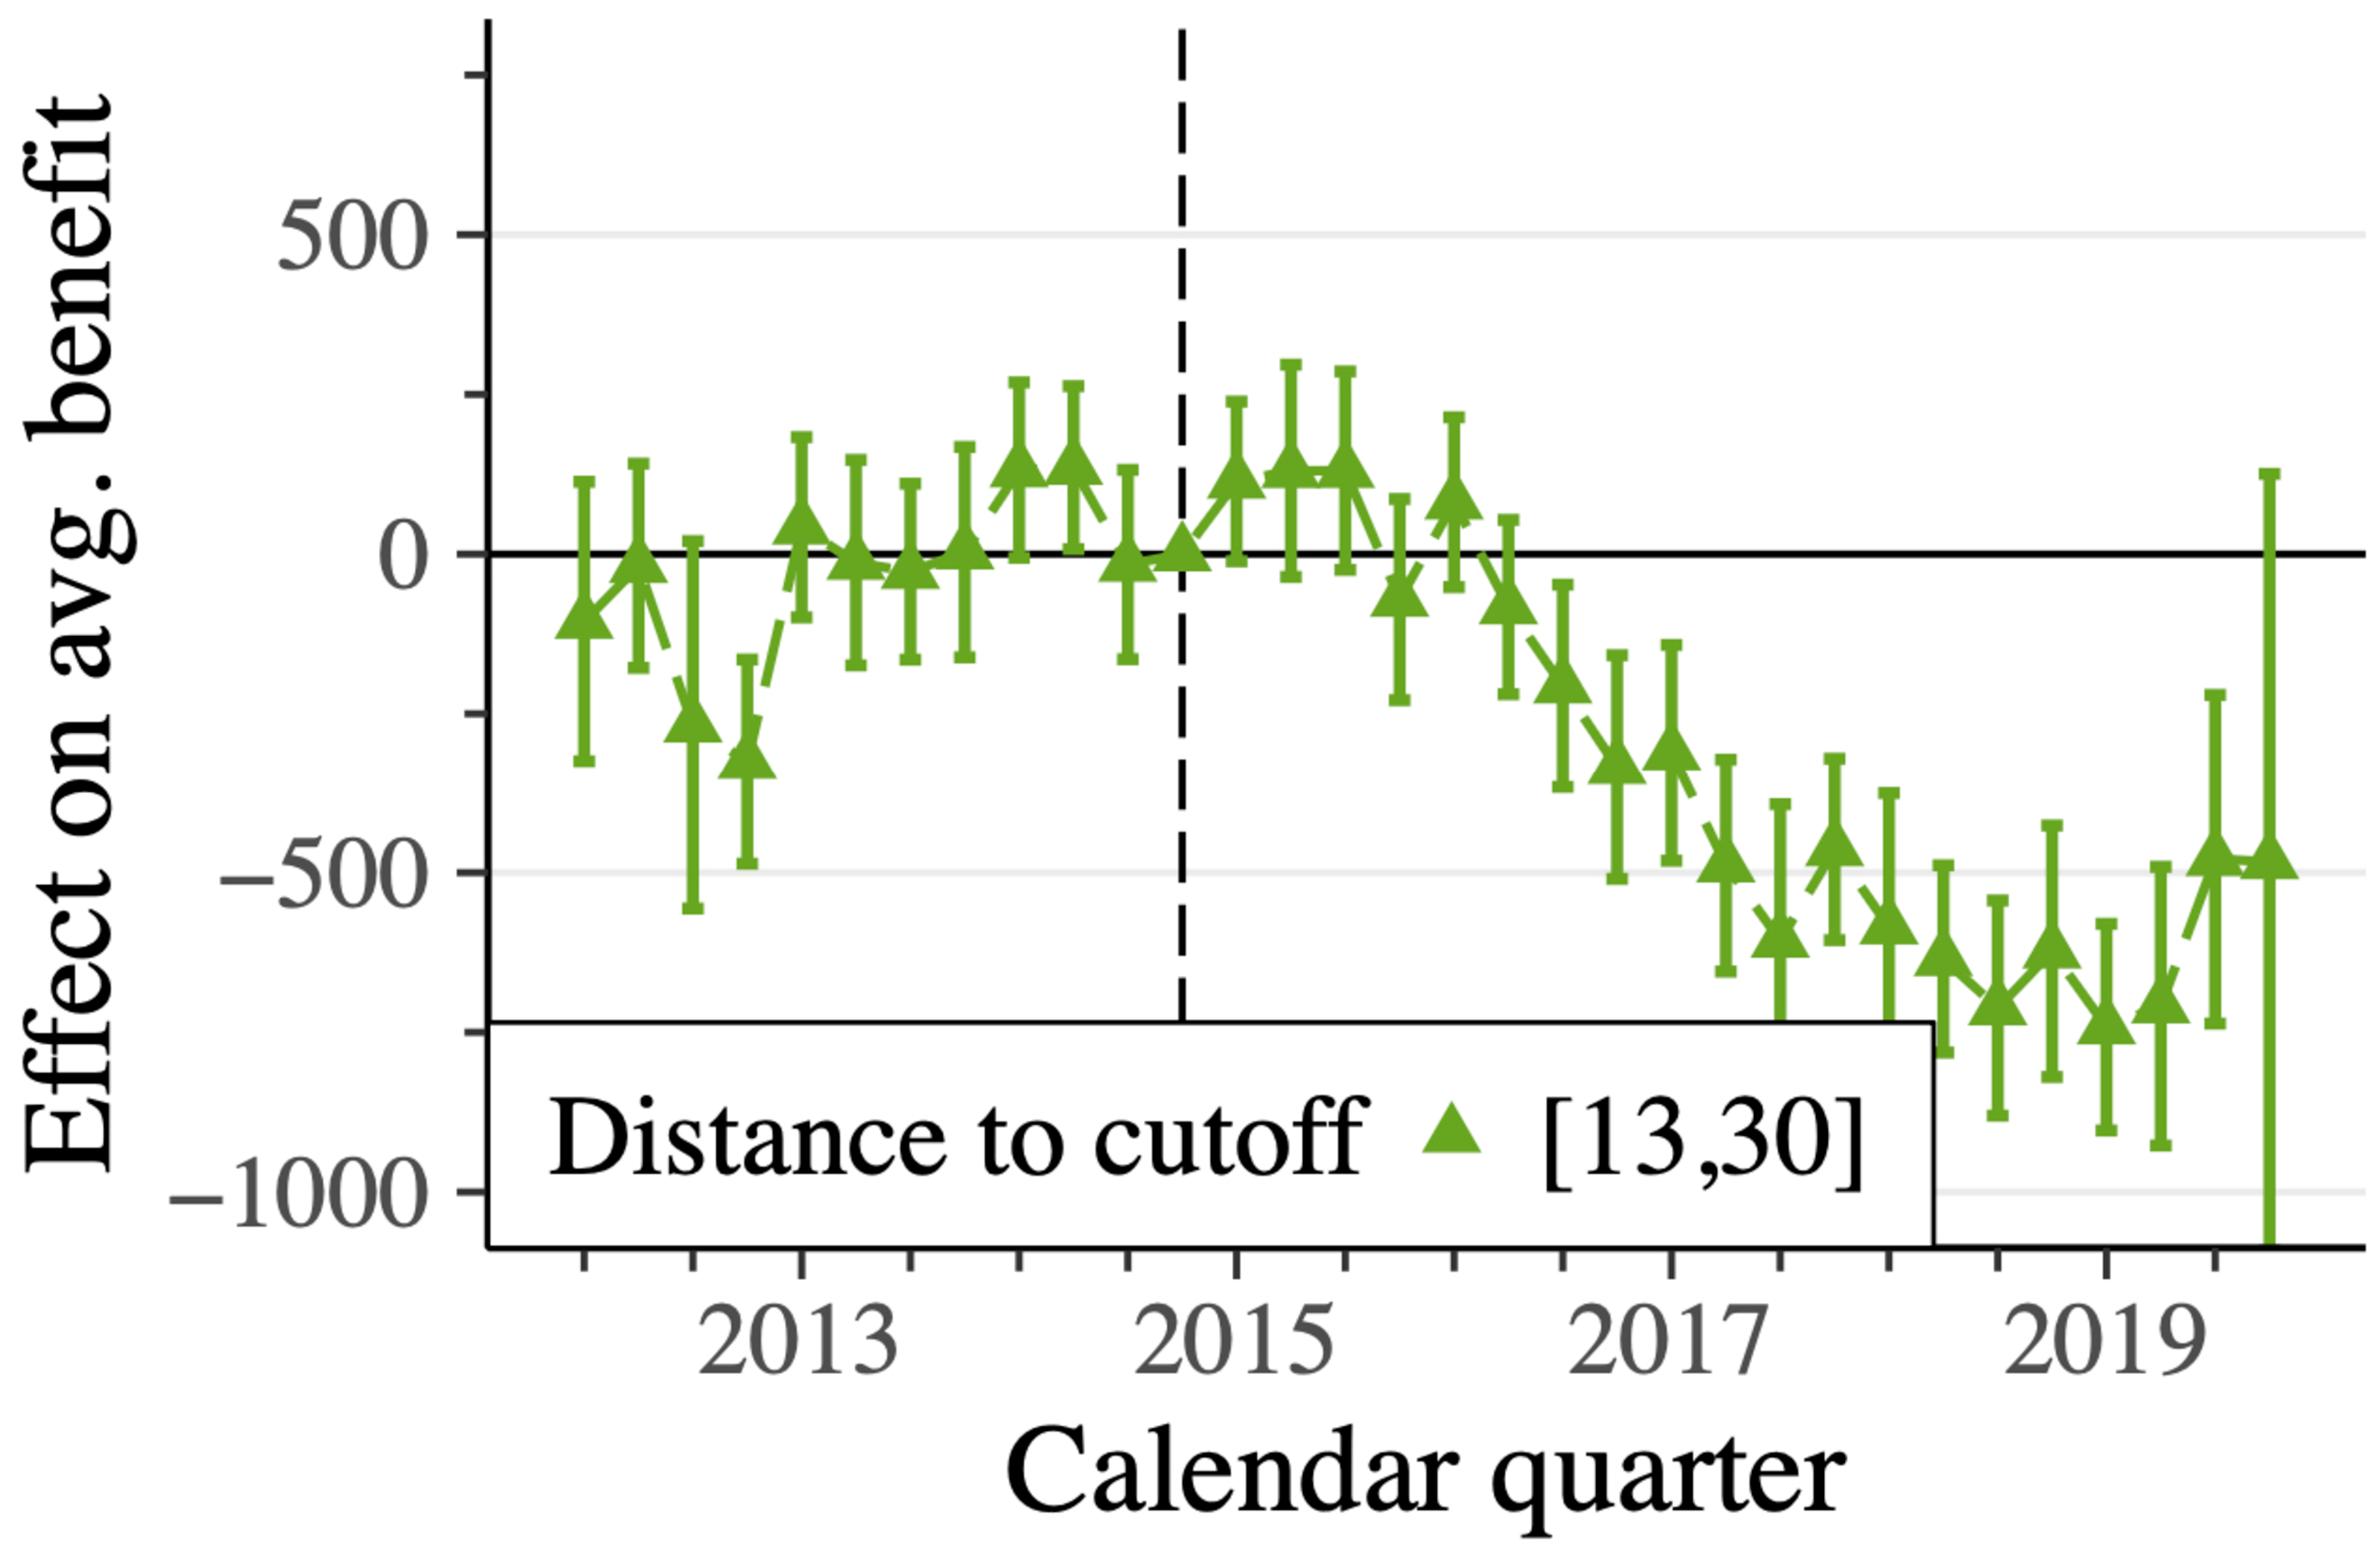
\includegraphics[width=0.8\linewidth]{new13.pdf}
    \bfootnote{\hyperlink{mechanicalRightAbove}{\beamerbutton{Voltar}}}
\end{frame}

\begin{frame}[label=netOfTaxBenefits]{Benefícios Contrafactuais Médios Líquidos de Impostos $\frac{1}{N_{p,t}^c}\sum_{i:p(x_{it}^c)=p}[b^c(x_{it}^c)-\tau(x^c_{it})]$}
    \begin{itemize}
        \item $\bar{b}^{NoT}_{p,t} \equiv \frac{1}{N_{p,t}} \sum_{i:p(x_{it}^a)=p}b^c(x_{it}^a)-\tau(x_{it}^a)$: média dos benefícios líquidos de impostos que teriam sido pagos aos que requerem com $p$ pontos normalizados no trimestre $t$ sob a regra pré-reforma e as escolhas pós-reforma
        \item Problema: os \textit{bunchers} podem ser positivamente selecionados (por exemplo, benefícios e impostos mais altos)
        \item Hipótese de identificação: $\bar{b}^{NoT}_{p,t}$ para $p\geq -6$ permaneceria paralelo ao observado em $p<-6$ na ausência da reforma
        \item O DiD recupera o efeito da reforma sobre esses benefícios médios $\beta^{NoT}_{k,p}$ em cada ponto normalizado $p$ e trimestre $k$:
         \begin{align*}
            \bar{b}^{NoT}_{p,t}=\delta_p^{NoT}+\gamma_t^{NoT} +\sum_{k\neq -2}\beta_{p,k}^{NoT} 1(p\in \tilde p)*1(t=k)+\varepsilon_{p,t}^{NoT}
        \end{align*}
        \item $\bar{b}^{NoT}_{p,t}-\hat \beta_{p,t}^{NoT}$ é uma estimativa de $\frac{1}{N_{p,t}^c}\sum_{i:p(x^c_{it})=p}[b^c(x^c_{it})-\tau(x^c_{it})]$
    \end{itemize}
    \bfootnote{\hyperlink{costReform}{\beamerbutton{Voltar}}}
    % The estimate for the average benefit that would have been paid in the absence of the reform at point p and quarter t is estimated as bar b^o_{p,t}-\beta_{t,p}
\end{frame}

\begin{frame}[label=theory]{Problema do Agente em Dois Estágios}
    \begin{align*}
        \tilde{U}_{i0}(p,b) =\max_{x_{i0}} \Big\{\sum_{t=0}^T\beta^t E[u(x_{it})]\ \text{sujeito à restrição orçamentária}, \\
         p(x^{iT})=p,\ \text{ e }\ b(x_{it})=b\Big\}
    \end{align*}
    \begin{itemize}
        \item $\tilde{U}_{i0}(p,b)$ é a utilidade esperada em forma reduzida em termos de pontos e benefícios, dadas escolhas racionais.
        \item Isso implica curvas de indiferença decrescentes em $\beta$ ($-\frac{d}{d\beta}\frac{d\tilde U/dp}{d\tilde U/db}<0$)
        \item Dois grupos de agentes:
        \begin{enumerate}
            \item Agentes não restritos: chegam à reforma com $p(x_{i0})<\bar p$ (podem fazer bunching em $\bar p$)
            \item Agentes restritos: chegam à reforma com $p(x_{i0})>\bar p$ pontos (não podem fazer bunching e só podem escolher em $[p(x_{i0}),\infty)$)
        \end{enumerate}
    \end{itemize}
    \bfootnote{\hyperlink{twoCounterfactualReforms}{\beamerbutton{Voltar}}}
\end{frame}

\begin{frame}[label=intuition]{Densidade Teórica Antes e Depois de $\Delta b_L>0$}
\centering
\setlength{\columnsep}{6pt}
\begin{columns}[T,onlytextwidth]

% ============= ESQUERDA =============
\begin{column}{0.49\textwidth}
\centering
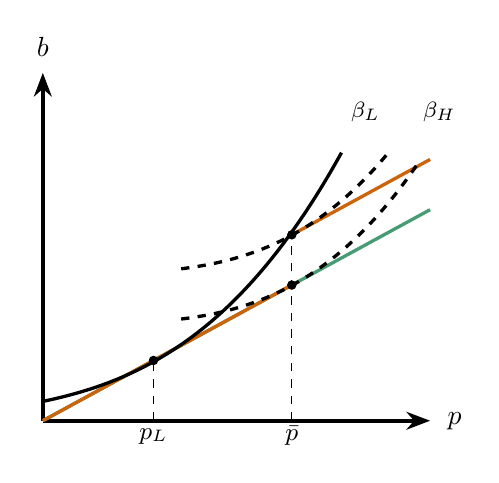
\begin{tikzpicture}
  \begin{axis}[
    width=6.5cm, height=6cm,
    axis lines=left,
    axis line style={-{Stealth[length=3mm]}, ultra thick},
    xmin=0, xmax=4.2, ymin=0, ymax=9,
    xtick=\empty, ytick=\empty, clip=false,
    %--- labels near arrow tips
    xlabel={$p$},
    xlabel style={at={(axis description cs:1.02,0)}, anchor=west},
    ylabel={}, % esvazia o ylabel do pgfplots (ele rotaciona por padrão)
  ]

    %--- Criamos manualmente o rótulo horizontal do eixo y no bico da seta:
    \node[anchor=south, rotate=0] at (axis description cs:0,1.02) {$b$};

    %---- Parâmetros
    \def\slope{1.3}
    \def\notch{1.3}
    \def\pH{1.2}
    \def\pbar{2.7}
    \def\aIC{0.08}

    %---- Linhas de orçamento (sempre visíveis)
    \addplot[very thick,col_before,domain=0:4.2] {\slope*x};
    \only<2->{\addplot[very thick,col_after,domain=0:\pbar] {\slope*x};
    \addplot[very thick,col_after,domain=\pbar:4.2] {\slope*x+\notch};
    \draw[dashed,black!60!black] (axis cs:\pbar,0) -- (axis cs:\pbar,\slope*\pbar+\notch);}

    %---- IC azul (sempre visível)
    \addplot[black, very thick, domain=0:4.1, samples=220, restrict y to domain=0:7]
      {1.5 + 0.5*(x-2) + 0.2*(x)^2 + 0.08*(x)^3};
    \filldraw[black] (axis cs:1.2,1.56) circle (1.5pt);
    \draw[dashed] (axis cs:1.2,0) -- (axis cs:1.2,1.56);
    \node[black] at (axis cs:3.5,8) {\footnotesize $\beta_L$};

    %---- IC vermelha baixa: aparece no overlay 2 (e já mostra \beta_H)
      \addplot[black, dashed, very thick, domain=1.5:4.1, samples=220, restrict y to domain=0:7.5]
        {3.5 + 1.3*(x-\pbar) + 0.6*(x-\pbar)^2 + 0.1*(x-\pbar)^3};
      \filldraw[black] (axis cs:2.7,3.51) circle (1.5pt);
      \draw[dashed] (axis cs:2.7,0) -- (axis cs:2.7,3.51);
      \node[black] at (axis cs:4.3,8) {\footnotesize $\beta_H$}; % já no overlay 2

    %---- IC vermelha alta: aparece no overlay 3
      \only<2->{\addplot[black, dashed, very thick, domain=1.5:4.1, samples=220, restrict y to domain=0:7]
        {4.8 + 1.3*(x-\pbar) + 0.6*(x-\pbar)^2 + 0.1*(x-\pbar)^3};
      \filldraw[black] (axis cs:2.7,4.81) circle (1.5pt);
      \draw[dashed] (axis cs:2.7,0) -- (axis cs:2.7,4.81);}

    %---- Rótulos no eixo x
    \node at (axis cs:{1.2},-0.4) {\small $p_L$};
    \node at (axis cs:{2.7},-0.4) {\small $\bar{p}$};

  \end{axis}
\end{tikzpicture}
\end{column}

% ============= DIREITA =============
\begin{column}{0.49\textwidth}
\centering

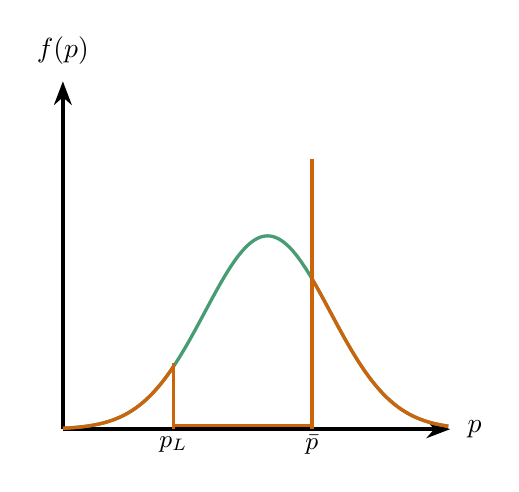
\begin{tikzpicture}
  \begin{axis}[
    width=6.5cm, height=6cm,
    axis lines=left,
    axis line style={-{Stealth[length=3mm]}, ultra thick},
    xmin=0, xmax=4.2, ymin=0, ymax=9,
    xtick=\empty, ytick=\empty, clip=false,
    %--- labels near arrow tips
    xlabel={$p$},
    xlabel style={at={(axis description cs:1.02,0)}, anchor=west},
    ylabel={}, % esvazia o ylabel do pgfplots (ele rotaciona por padrão)
  ]

    %--- Criamos manualmente o rótulo horizontal do eixo y no bico da seta:
    \node[anchor=south, rotate=0] at (axis description cs:0,1.02) {$f(p)$};

    \addplot[very thick, col_before, domain=0:4.18, samples=220, smooth]
      {5 * exp(-0.5*((x-2.22)/0.68)^2)};

    \only<2->{\addplot[very thick, col_after, domain=0:1.2, samples=220, smooth]
      {5 * exp(-0.5*((x-2.22)/0.68)^2)};

      \addplot[very thick, col_after, domain=2.7:4.18, samples=220, smooth]
      {5 * exp(-0.5*((x-2.22)/0.68)^2)};

    \draw[very thick, col_after] (axis cs:1.2,0) -- (axis cs:1.2,1.7);
    \draw[very thick, col_after] (axis cs:1.2,0.1) -- (axis cs:2.7,0.1);
    \draw[ultra thick, col_after] (axis cs:2.7,0) -- (axis cs:2.7,7);}

    %---- Rótulos no eixo x
    \node at (axis cs:{1.2},-0.4) {\small $p_L$};
    \node at (axis cs:{2.7},-0.4) {\small $\bar{p}$};

  \end{axis}
\end{tikzpicture}


\end{column}
\end{columns}
\end{frame}

\begin{frame}[label=intuitionSlope]{Densidade Teórica Antes e Depois de $\Delta b_S<0$}
\centering
\setlength{\columnsep}{6pt}
\begin{columns}[T,onlytextwidth]

% ============= ESQUERDA =============
\begin{column}{0.49\textwidth}
\centering

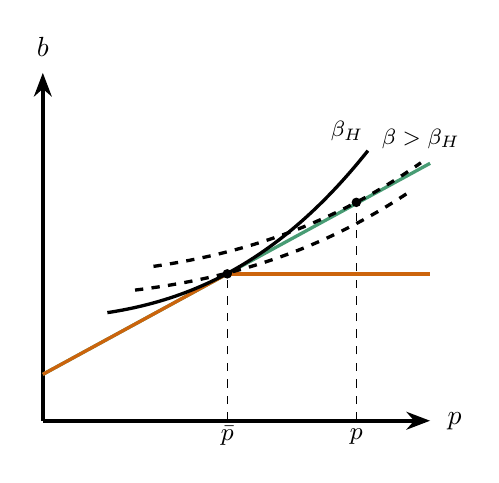
\begin{tikzpicture}
  \begin{axis}[
    width=6.5cm, height=6cm,
    axis lines=left,
    axis line style={-{Stealth[length=3mm]}, ultra thick},
    xmin=0, xmax=4.2, ymin=0, ymax=9,
    xtick=\empty, ytick=\empty, clip=false,
    %--- labels near arrow tips
    xlabel={$p$},
    xlabel style={at={(axis description cs:1.02,0)}, anchor=west},
    ylabel={}, % esvazia o ylabel do pgfplots (ele rotaciona por padrão)
  ]

    %--- Criamos manualmente o rótulo horizontal do eixo y no bico da seta:
    \node[anchor=south, rotate=0] at (axis description cs:0,1.02) {$b$};

    %---- Parâmetros
    \def\slope{1.3}
    \def\notch{1.3}
    \def\pH{1.2}
    \def\pbar{2.7}
    \def\aIC{0.08}

    %---- Linhas de orçamento (sempre visíveis)
    \addplot[very thick,col_before,domain=0:4.2] {1.2+\slope*x};
    \only<2>{\addplot[very thick,col_after,domain=0:2] {1.2+\slope*x};}
    \only<2>{\addplot[very thick,col_after,domain=2:4.2] {1.2+\slope*2};}
    \draw[dashed,black!60!black] (axis cs:2,0) -- (axis cs:2,1.2+\slope*2);

    %---- IC solida (sempre visível)
    \addplot[black, very thick, domain=0.7:4.1, samples=220, restrict y to domain=0:7]
      {2.65 + 0.08*x + 0.15*x^(2) + 0.05*x^(3)};
    \filldraw[black] (axis cs:2,1.2+\slope*2) circle (1.5pt);
    \node[black] at (axis cs:3.3,7.5) {\footnotesize $\beta_H$};

    %---- IC dashed - before
    \addplot[black, dashed, very thick, domain=1.2:4.1, samples=220, restrict y to domain=0:7]
      {3.75+0.09*x+0.07*x^(2)+0.02*x^(3)};
    \filldraw[black] (axis cs:3.4,5.65) circle (1.5pt);
    \node[black] at (axis cs:4.1,7.3) {\footnotesize $\beta > \beta_H$};
    \draw[dashed,black!60!black] (axis cs:3.4,0) -- (axis cs:3.4,5.65);

    %---- IC dashed - after
    \only<2>{\addplot[black, dashed, very thick, domain=1:4, samples=220, restrict y to domain=0:7]
      {3.2+0.09*x+0.07*x^(2)+0.02*x^(3)};}

    %---- Rótulos no eixo x
    \node at (axis cs:{2},-0.4) {\small $\bar p$};
    \node at (axis cs:{3.4},-0.4) {\small $p$};

  \end{axis}
\end{tikzpicture}

\end{column}

% ============= DIREITA =============
\begin{column}{0.49\textwidth}
\centering

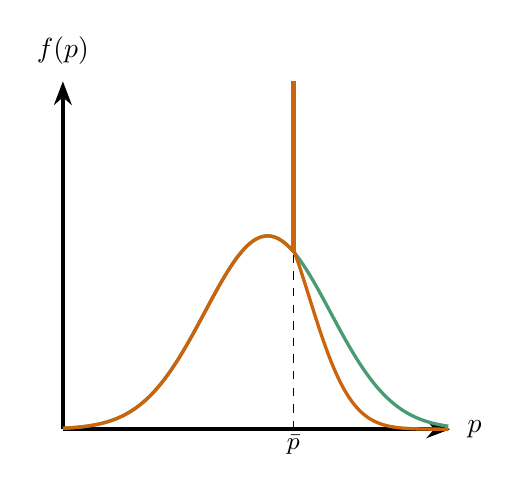
\begin{tikzpicture}
  \begin{axis}[
    width=6.5cm, height=6cm,
    axis lines=left,
    axis line style={-{Stealth[length=3mm]}, ultra thick},
    xmin=0, xmax=4.2, ymin=0, ymax=9,
    xtick=\empty, ytick=\empty, clip=false,
    %--- labels near arrow tips
    xlabel={$p$},
    xlabel style={at={(axis description cs:1.02,0)}, anchor=west},
    ylabel={}, % esvazia o ylabel do pgfplots (ele rotaciona por padrão)
  ]

    %--- Criamos manualmente o rótulo horizontal do eixo y no bico da seta:
    \node[anchor=south, rotate=0] at (axis description cs:0,1.02) {$f(p)$};

    \addplot[very thick, col_before, domain=0:4.18, samples=220, smooth]
      {5 * exp(-0.5*((x-2.22)/0.68)^2)};

    \only<2>{\addplot[very thick, col_after, domain=0:2.5, samples=220, smooth]
      {5 * exp(-0.5*((x-2.22)/0.68)^2)};}

    \only<2>{\addplot[very thick, col_after, domain=2.5:4.18, samples=220, smooth]
      {5.65 * exp(-0.5*((x-2.22)/0.45)^2)};}

    \only<2>{\draw[ultra thick, col_after] (axis cs:2.5,4.6) -- (axis cs:2.5,9);}

    \draw[dashed,black!60!black] (axis cs:2.5,0) -- (axis cs:2.5,4.6);

    %---- Rótulos no eixo x
    \node at (axis cs:{2.5},-0.4) {\small $\bar{p}$};

  \end{axis}
\end{tikzpicture}


\end{column}
\end{columns}
% This movement happens over time because unconstrained individuals with ideal points at p>pbar may have to wait quarters after the reform to reach pbar and bunch. 
    % Ex: Woman with p^sim=80 at t=0 and works needs to wait 2.5 years (til december 2017) to claim. 
    % She would have claimed with 86 points in june 2018 but claims now with 85 in december 2017. 
    % Her movement increases claiming at 2017Q4 at pbar, so that the counterfactual claiming in 2017Q4 at pbar is lower than the actual 
    % But it also decreases claiming at 2018Q2 at p=85, so that the counterfactual claiming in 2018Q2 is higher than the actual claiming.  
    % Note this effect on pbar+x takes x/2 years to happen or 2x quarter to happen. So for example, a movement from pbar + 6 to pbar would take 12 quarters to appear (there are 12 quarters between the reform and 2018Q2)
    \bfootnote{\hyperlink{constrained}{\beamerbutton{Agentes Restritos}} \hyperlink{twoCounterfactualReforms}{\beamerbutton{Voltar}}}
\end{frame}

\begin{frame}[label=constrained]{Agentes Restritos Respondendo a $\Delta b_S$}
    \centering 
    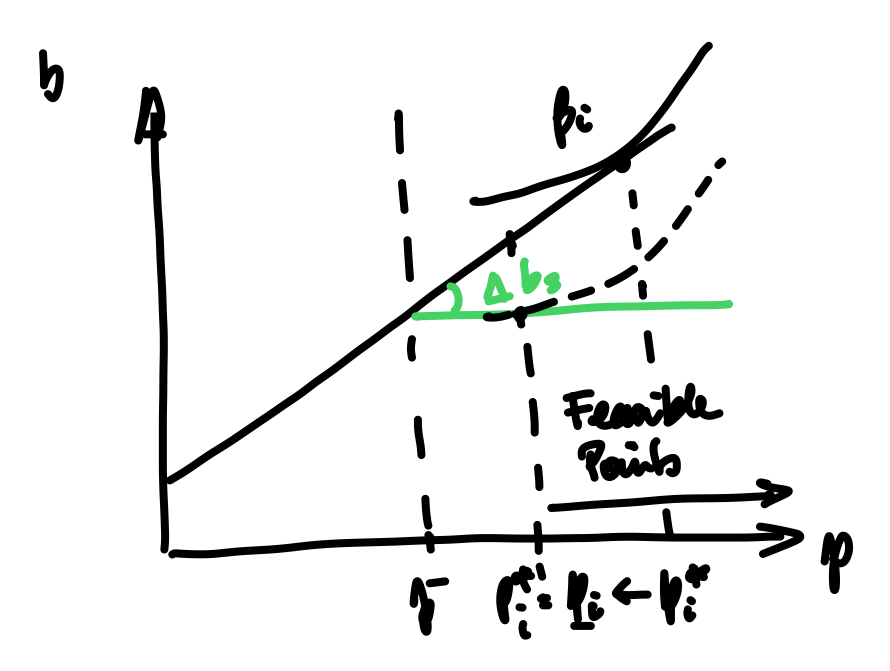
\includegraphics[width=.8\textwidth]{morRef2The.png}
    % This response should increase the claiming density at p_underline immediately after the reform. (Only people are inattentive; this effect could be delayed.)
    % It should also decrease the claiming density at  p*=p_underline+x, x/2 years or 2x quarters after the reform. Ex: If punderline=87 and p*=89 (x=2), it should decrease density in 89 four quarters after the reform (.
    % There should be no one claiming at p>pbar after the first quarter after the reform unless it is because of frictions.
    % Note that if there are partial frictions (people claim at pbar+epsilon<p*), then the increase will happen at pbar+epsilon, 2*epsilon quarters after the reform. The decrease in p* should happen in the same period. 
    % Empiricamente, não conseguimos estimar o efeito sobre a CHs so para constrained agents (those that have age+contribution>pbar in June 2015), because the CH is not defined for those that have already claimed. So after the reform, there will be no one claiming with p<pbar-6.5 because everyone will be claiming with p>age+contribution in June 2015. 
    % Idea: plot the distribution of constrained agents at each month before and after the reform. I think the logic above has predictions for where (points) and when (quarters) the effect should arise. 
    \bfootnote{\hyperlink{twoCounterfactualReforms}{\beamerbutton{Voltar}}}
\end{frame}

\begin{frame}{\textcolor{red}{Frequências das Reformas Puras: Anúncio ($t=-1$)}}
\begin{itemize}
    \item Para $p<0$, há apenas postergação que ocorreria sob a reforma pura em nível, mas não sob a reforma pura em inclinação. Portanto:
    \[
    N^L_{p,-1}=N^a_{p,-1}
    \qquad\text{and}\qquad
    N^S_{p,-1}=N^c_{p,-1}
    \]
    \item Para $p\geq 0$, a reforma observada induz postergação em $t=-1$ devido aos maiores benefícios pós-reforma (como na reforma pura em nível)
    \item Portanto, para requerentes já elegíveis:
    \[
    N^L_{p,-1}=N^a_{p,-1}, \qquad p\geq 0
    \]
\end{itemize}
\end{frame}

\begin{frame}{\textcolor{red}{Antecipação na Reforma Pura em Inclinação em $t=-1$: Lógica}}
\begin{itemize}
    \item Sob a reforma pura em inclinação, o aumento de nível não existe e esperar se torna menos atraente para $p>0$
    \item Assim, requerentes já elegíveis que atrasam sob a reforma observada passariam a antecipar sob a reforma pura em inclinação
    \item A1 (Mapeamento de Atenção): se um indivíduo reage com atraso de $x$ trimestres após a implementação na reforma observada, ele reagiria com atraso de $x$ trimestres após o anúncio na reforma pura em inclinação
    \begin{itemize}
        \item Isso implica que a massa excedente inicial sob a reforma observada em $t$ é deslocada para $t-1$ sob a reforma pura em inclinação
    \end{itemize}
    \item Como os pontos aumentam em $0.5$ por trimestre, enquanto $p$ é agrupado em inteiros, a massa de $(p,0)$ é redistribuída para $(p,-1)$ e $(p-1,-1)$ para $p\geq 0$
\end{itemize}
\end{frame}

\begin{frame}{\textcolor{red}{Frequências da Reforma Pura em Inclinação em $t=-1$ e $p\geq 0$}}
    \begin{itemize}
        \item Defina a massa excedente inicial na célula $(p,t)$ como $EM_{p,t}\equiv N^a_{p,t}-N^c_{p,t}$
        \item A1 implica que a massa de antecipação que entra em $p\geq 0$ e $t=-1$ é:
        \[
        A_{p,-1}\equiv \frac12 EM_{p,0}+\frac12 EM_{p+1,0}.
        \]
        \item Para $p\geq 0$ e $t=-1$, a frequência sob a reforma pura em inclinação é igual à distribuição contrafactual (já que ninguém postergaria) mais essa massa de antecipação (já que os antecipadores requereriam antes da reforma):
        \begin{align*}
            N^S_{p,-1}=N^c_{p,-1}+A_{p,-1}
        \end{align*}
    \end{itemize}
\end{frame}

\begin{frame}{Hipóteses: Acumulação de Pontos e Janela de Bunching}
\begin{itemize}
    \item A3: o bunching só ocorre em $p\in[0,\textcolor{red}{3})$, correspondendo a respostas nos \textcolor{red}{3} primeiros trimestres após o primeiro contato com o incentivo
    \item Nos primeiros trimestres pós-reforma, pode surgir massa excedente além de $p=2$ porque a antecipação dos requerentes já elegíveis é difusa
    \item A restrição empírica central é que esse excesso em $p$ mais alto desaparece em grande medida após $t=\textcolor{red}{3}$
    \item Isso motiva usar massa excedente inicial apenas para $t\in\{0,1,2,3\}$ ao construir a antecipação da reforma pura em inclinação
\end{itemize}
\end{frame}

\begin{frame}[label=pureLStep]{Separando Respostas: Visão Geral}
    \begin{itemize}
        \item Estimamos os efeitos de bem-estar dessas reformas puras em 5 etapas
        \begin{enumerate}
            \item \alt<2>{\textbf{Estimar frequências sob a reforma pura em nível, redistribuindo a massa faltante de postergação para regiões futuras de bunching}}{Estimar frequências sob a reforma pura em nível, redistribuindo a massa faltante de postergação para regiões futuras de bunching}
            \item Estimar frequências sob a reforma pura em inclinação, removendo do bunching observado a postergação encontrada em (1)
            \item Estimar os gastos mecânicos sob ambas as reformas, sem respostas, corrigindo por toda a seleção
            \item Estimar os gastos sob cada reforma, corrigindo apenas pela seleção associada à antecipação (postergação)
            \item Calcular efeitos de bem-estar e custos totais a partir de 1-4 e então calcular os WMVPFs
        \end{enumerate}
    \end{itemize}
    \bfootnote{\hyperlink{pureL}{\beamerbutton{Detalhes das Frequências da Reforma Pura em Nível}}}
\end{frame}

\begin{frame}{Frequências sob a Reforma Pura em \textbf{Nível}:
    \only<1>{Q3 2015}\only<2>{Q4 2015}\only<3>{Q1 2016}\only<4>{Q2 2016}\only<5>{Q3 2016}\only<6>{Q4 2016}\only<7>{Q1 2017}\only<8>{Q2 2017}\only<9>{Q3 2017}\only<10>{Q4 2017}\only<11>{Q1 2018}\only<12>{Q2 2018}\only<13>{Q3 2018}}
     \only<1>{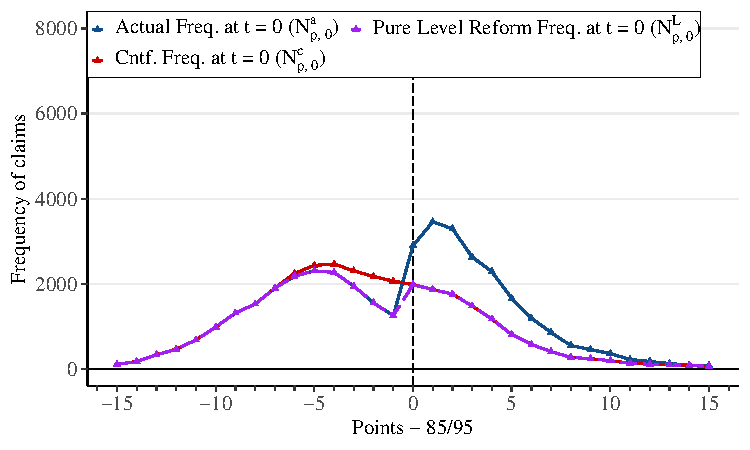
\includegraphics[width=.9\linewidth]{frequenciesLQ0.pdf}}\only<2>{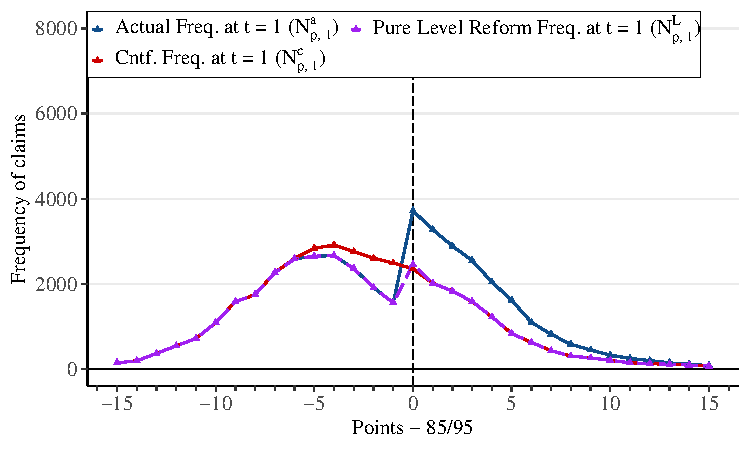
\includegraphics[width=.9\linewidth]{frequenciesLQ1.pdf}}\only<3>{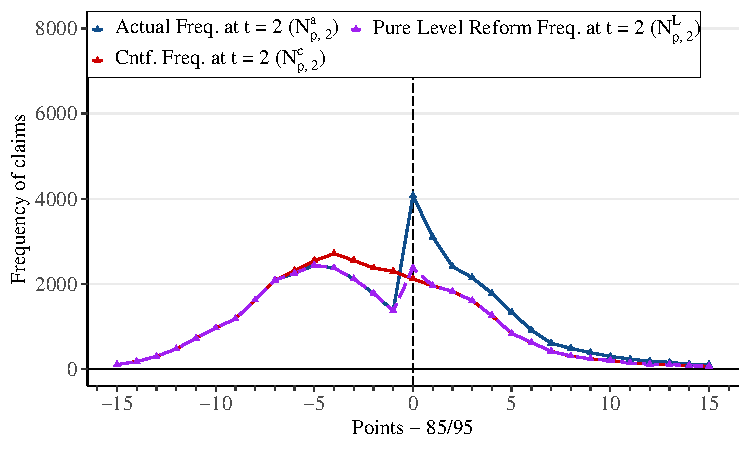
\includegraphics[width=.9\linewidth]{frequenciesLQ2.pdf}}\only<4>{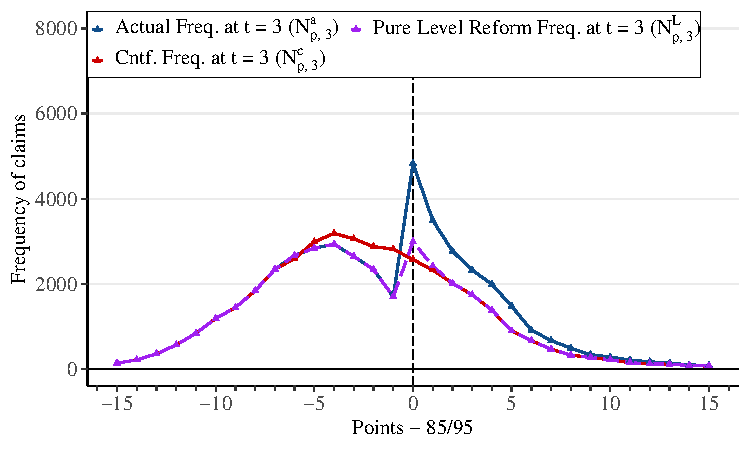
\includegraphics[width=.9\linewidth]{frequenciesLQ3.pdf}}\only<5>{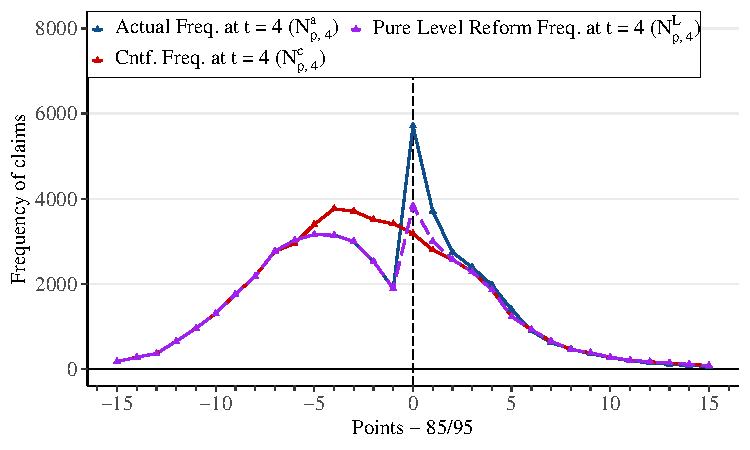
\includegraphics[width=.9\linewidth]{frequenciesLQ4.pdf}}\only<6>{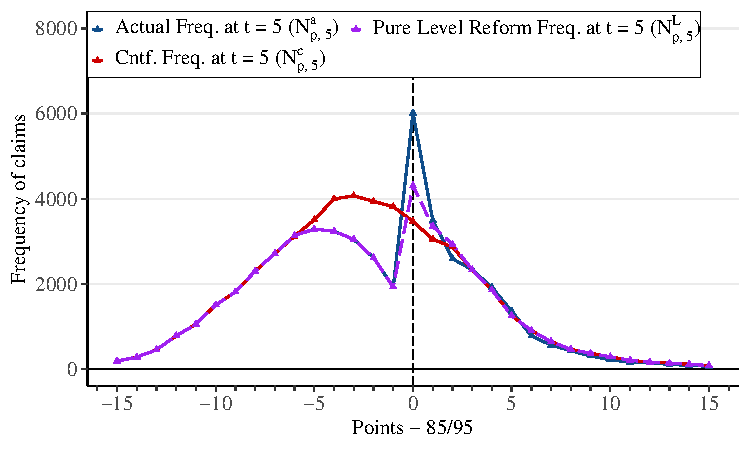
\includegraphics[width=.9\linewidth]{frequenciesLQ5.pdf}}\only<7>{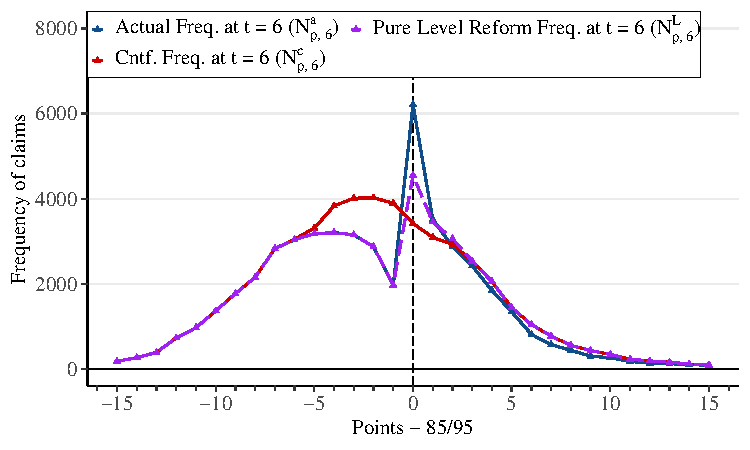
\includegraphics[width=.9\linewidth]{frequenciesLQ6.pdf}}\only<8>{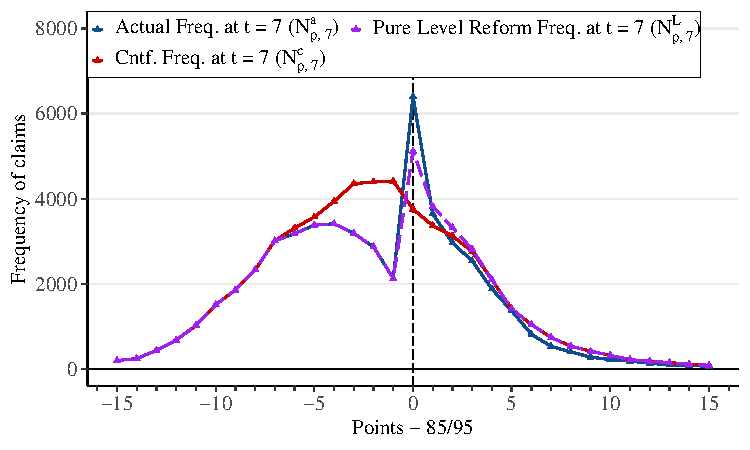
\includegraphics[width=.9\linewidth]{frequenciesLQ7.pdf}}\only<9>{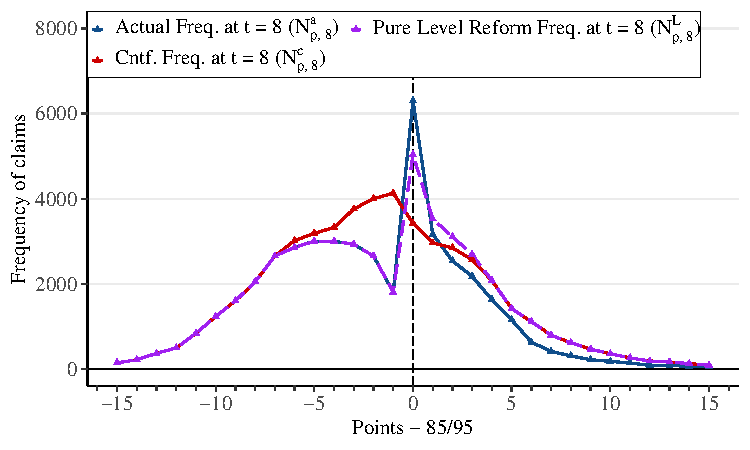
\includegraphics[width=.9\linewidth]{frequenciesLQ8.pdf}}\only<10>{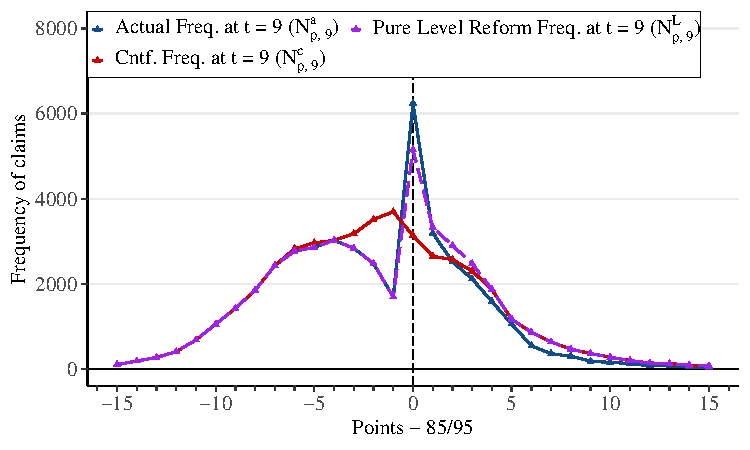
\includegraphics[width=.9\linewidth]{frequenciesLQ9.pdf}}\only<11>{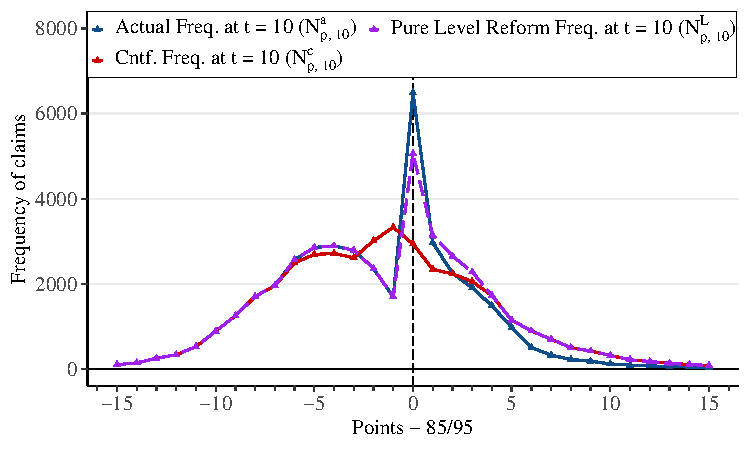
\includegraphics[width=.9\linewidth]{frequenciesLQ10.pdf}}\only<12>{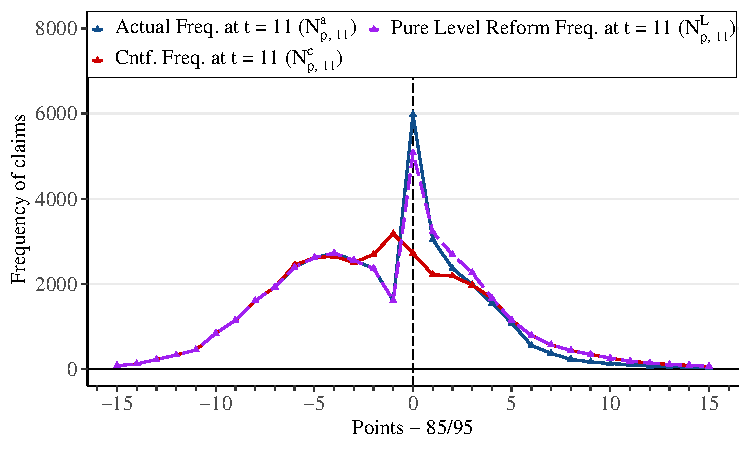
\includegraphics[width=.9\linewidth]{frequenciesLQ11.pdf}}\only<13>{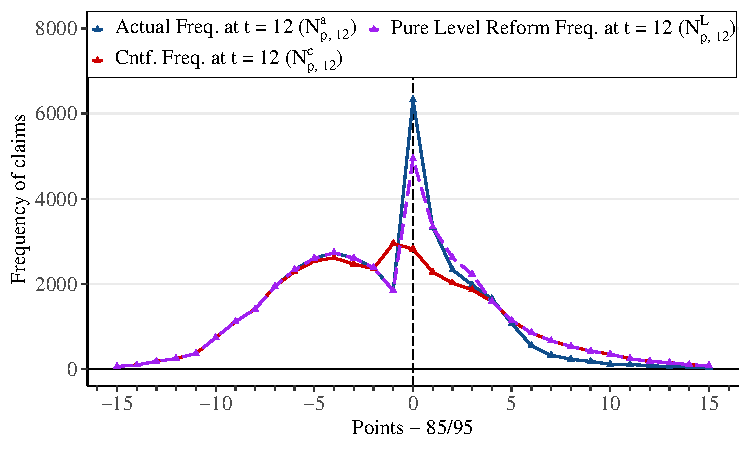
\includegraphics[width=.9\linewidth]{frequenciesLQ12.pdf}}
\end{frame}

\begin{frame}[label=pureSStep]{Separando Respostas: Visão Geral}
    \begin{itemize}
        \item Estimamos os efeitos de bem-estar dessas reformas puras em 5 etapas
        \begin{enumerate}
            \item Estimar frequências sob a reforma pura em nível, redistribuindo a massa faltante de postergação para regiões futuras de bunching
            \item \alt<2>{\textbf{Estimar frequências sob a reforma pura em inclinação, removendo do bunching observado a postergação encontrada em (1)}}{Estimar frequências sob a reforma pura em inclinação, removendo do bunching observado a postergação encontrada em (1)}
            \item Estimar os gastos mecânicos sob ambas as reformas, sem respostas, corrigindo por toda a seleção
            \item Estimar os gastos sob cada reforma, corrigindo apenas pela seleção associada à antecipação (postergação)
            \item Calcular efeitos de bem-estar e custos totais a partir de 1-4 e então calcular os WMVPFs
        \end{enumerate}
    \end{itemize}
    \bfootnote{\hyperlink{pureS}{\beamerbutton{Detalhes das Frequências da Reforma Pura em Inclinação}}}
\end{frame}

\begin{frame}{Frequências sob a Reforma Pura em \textbf{Inclinação}:
    \only<1>{Q3 2015}\only<2>{Q4 2015}\only<3>{Q1 2016}\only<4>{Q2 2016}\only<5>{Q3 2016}\only<6>{Q4 2016}\only<7>{Q1 2017}\only<8>{Q2 2017}\only<9>{Q3 2017}\only<10>{Q4 2017}\only<11>{Q1 2018}\only<12>{Q2 2018}\only<13>{Q3 2018}}
     \only<1>{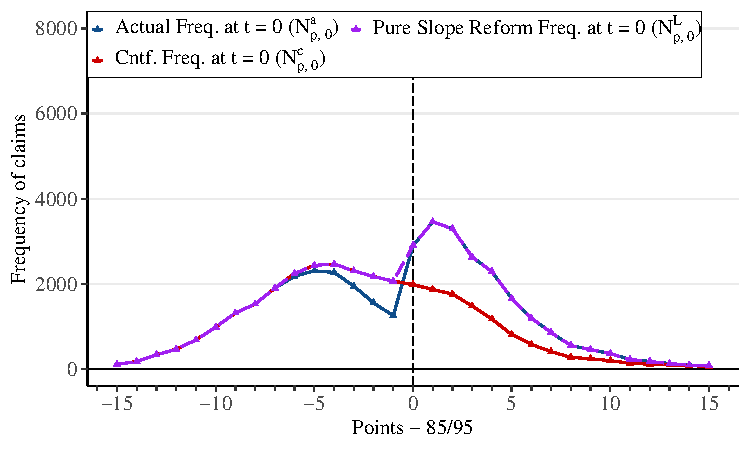
\includegraphics[width=.9\linewidth]{frequenciesSQ0.pdf}}\only<2>{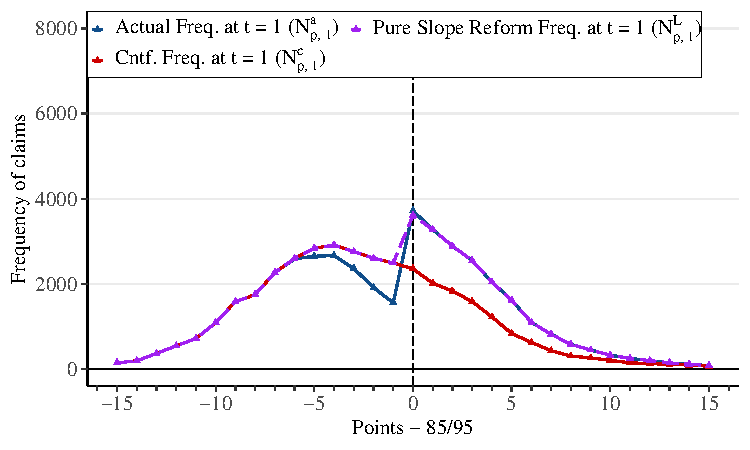
\includegraphics[width=.9\linewidth]{frequenciesSQ1.pdf}}\only<3>{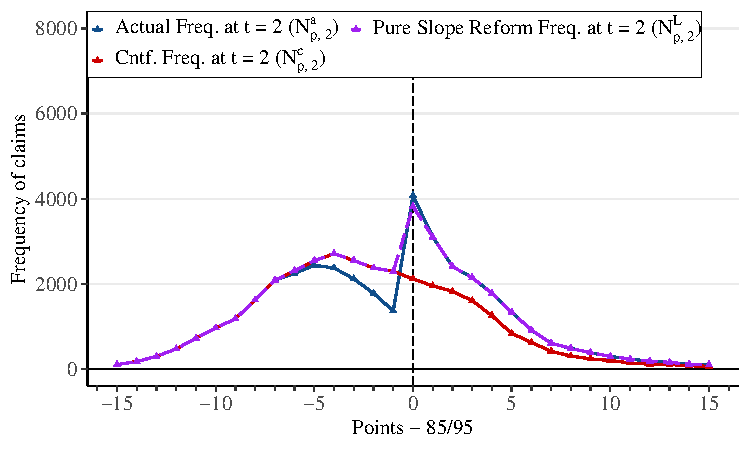
\includegraphics[width=.9\linewidth]{frequenciesSQ2.pdf}}\only<4>{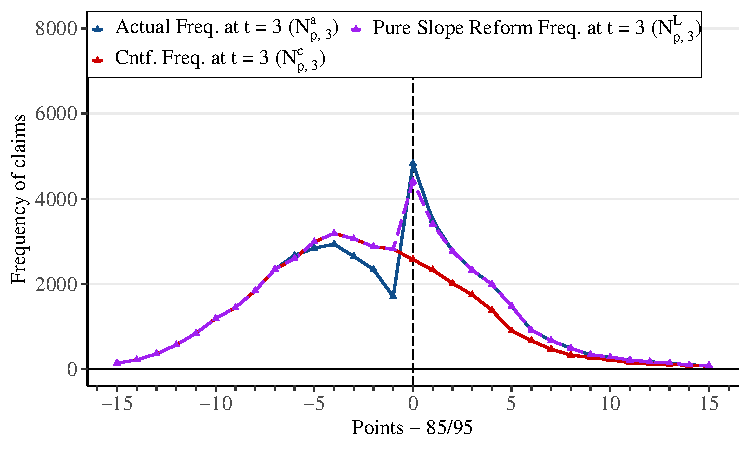
\includegraphics[width=.9\linewidth]{frequenciesSQ3.pdf}}\only<5>{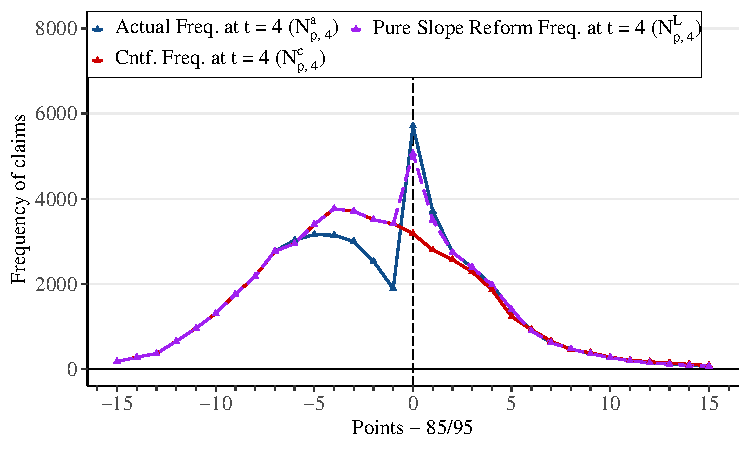
\includegraphics[width=.9\linewidth]{frequenciesSQ4.pdf}}\only<6>{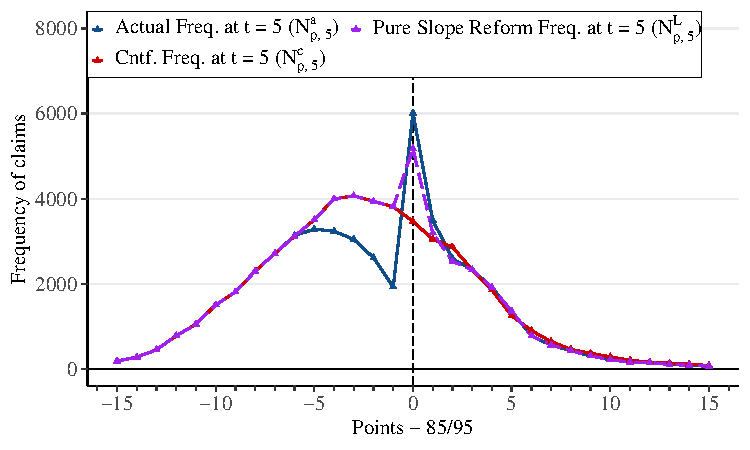
\includegraphics[width=.9\linewidth]{frequenciesSQ5.pdf}}\only<7>{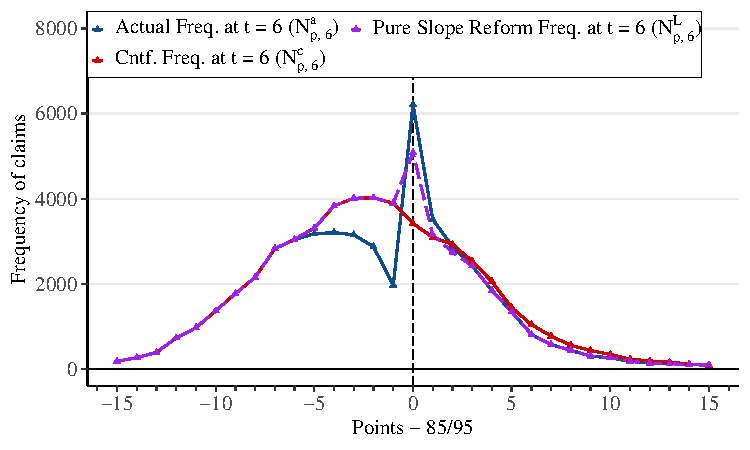
\includegraphics[width=.9\linewidth]{frequenciesSQ6.pdf}}\only<8>{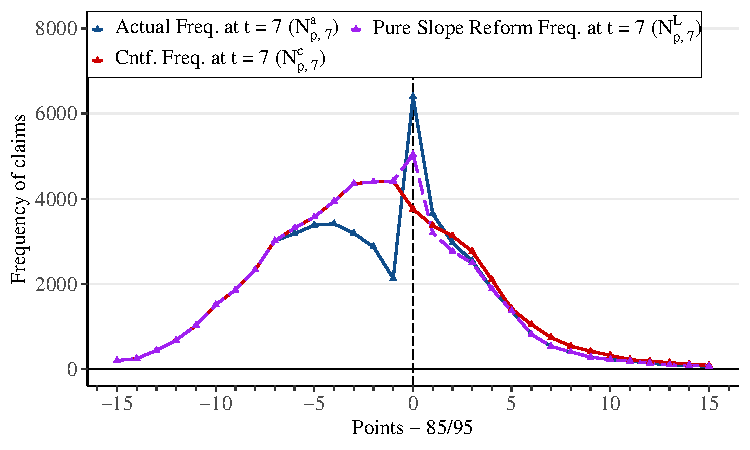
\includegraphics[width=.9\linewidth]{frequenciesSQ7.pdf}}\only<9>{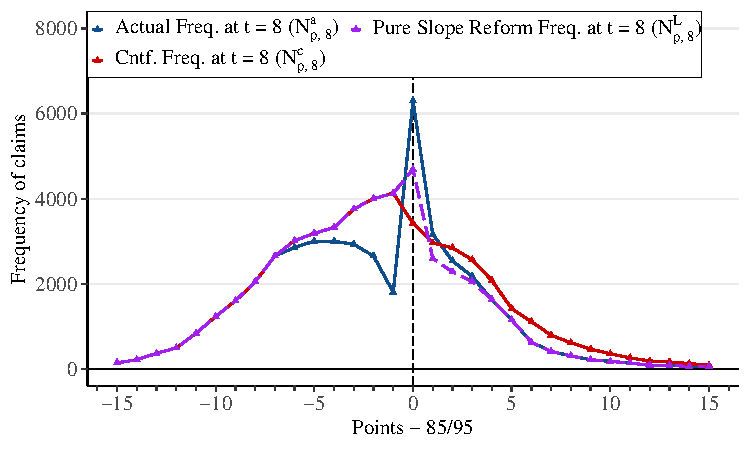
\includegraphics[width=.9\linewidth]{frequenciesSQ8.pdf}}\only<10>{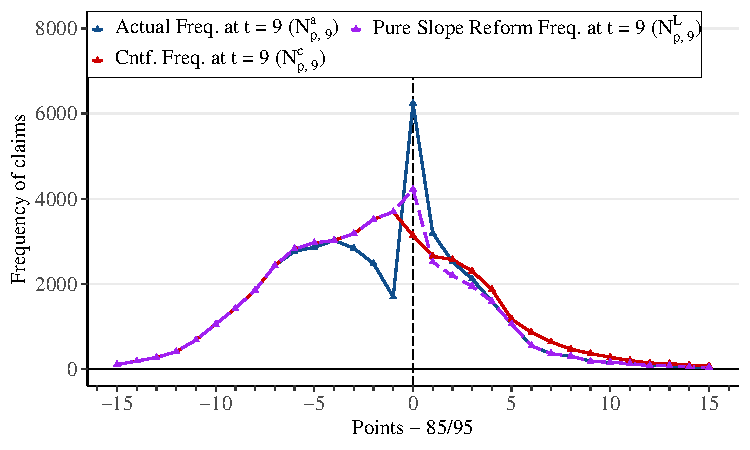
\includegraphics[width=.9\linewidth]{frequenciesSQ9.pdf}}\only<11>{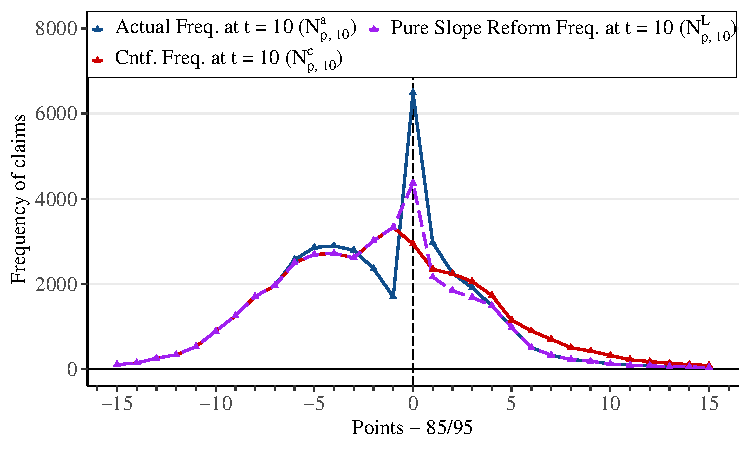
\includegraphics[width=.9\linewidth]{frequenciesSQ10.pdf}}\only<12>{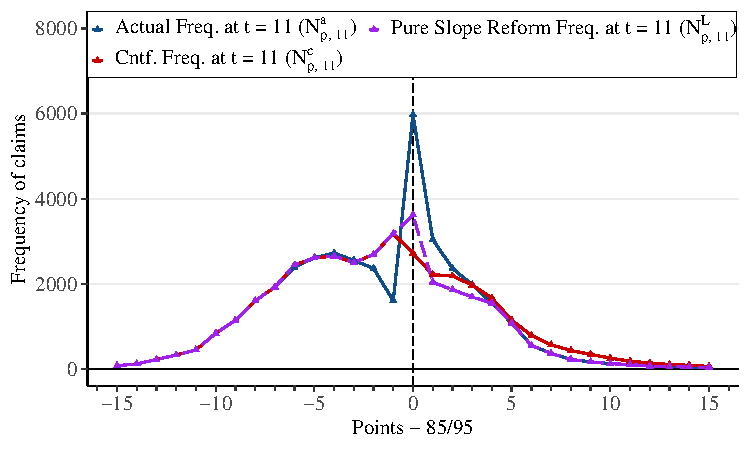
\includegraphics[width=.9\linewidth]{frequenciesSQ11.pdf}}\only<13>{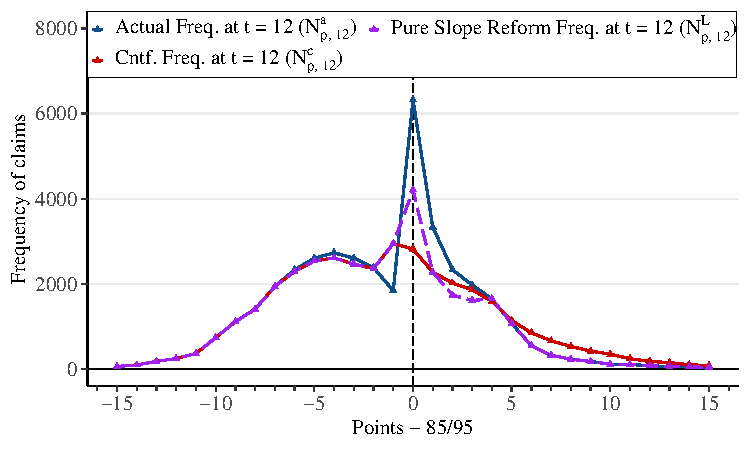
\includegraphics[width=.9\linewidth]{frequenciesSQ12.pdf}}
\end{frame}
    
\begin{frame}[label=disentangling]{Separando Respostas: Visão Geral}
    \begin{itemize}
        \item Estimamos os efeitos de bem-estar dessas reformas puras em 5 etapas
        \begin{enumerate}
            \item Estimar frequências sob a reforma pura em nível, redistribuindo a massa faltante de postergação para regiões futuras de bunching
            \item Estimar frequências sob a reforma pura em inclinação, removendo do bunching observado a postergação encontrada em (1)
            \item \alt<2>{\textbf{Estimar os gastos mecânicos sob ambas as reformas, sem respostas, corrigindo por toda a seleção}}{Estimar os gastos mecânicos sob ambas as reformas, sem respostas, corrigindo por toda a seleção}
            \item \alt<2>{\textbf{Estimar os gastos sob cada reforma, corrigindo apenas pela seleção associada à antecipação (postergação)}}{Estimar os gastos sob cada reforma, corrigindo apenas pela seleção associada à antecipação (postergação)}
            \item \alt<2>{\textbf{Calcular efeitos de bem-estar e custos totais a partir de 1-4 e então calcular os WMVPFs}}{Calcular efeitos de bem-estar e custos totais a partir de 1-4 e então calcular os WMVPFs}
        \end{enumerate}
    \end{itemize}
    \bfootnote{\hyperlink{pureDetails}{\beamerbutton{Detalhes}}}
\end{frame}

\section{Reforma Ótima}

\begin{frame}[label=optimal]{Reforma Ótima com Orçamento Balanceado}
    \begin{itemize}
        \item Qual reforma da regra aumenta mais o bem-estar?
        \begin{itemize}
            \item Local no sentido de que o governo só pode aumentar custos e receitas em um montante fixo igual a $C(b^c,b^a)\approx R\$250$ bi
        \end{itemize}
        \item Vantagem de implementação:
        \begin{itemize}
            \item A \textbf{regra} previdenciária ótima depende de estatísticas suficientes sob a regra \textbf{ótima}
            \item A \textbf{reforma} previdenciária ótima depende de estatísticas suficientes sob a regra \textbf{observada}
        \end{itemize}
        \item $WMVPF_{b_L} \approx 0.68<0.71\approx WMVPF_{b_S}$
        \begin{itemize}
            \item $\Delta b_S^*=0.081$: aumento de 350\% (a linha de base era 0.023)
            \item $\Delta b_L^*=-791$: queda de 26\% (a linha de base era 3014.76)
        \end{itemize}
    \end{itemize}
    \bfootnote{\hyperlink{optimalDetails}{\beamerbutton{Detalhes}}}
\end{frame}

\begin{frame}{Reforma Ótima Neutra em Orçamento}
\centering
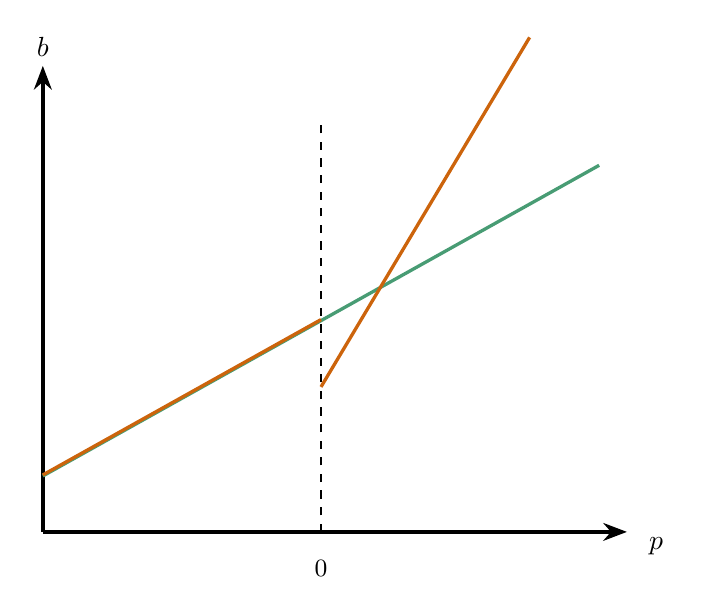
\begin{tikzpicture}
  \begin{axis}[
    width=9cm, height=7.5cm,
    axis lines=left,
    axis line style={-{Stealth[length=3mm]}, ultra thick},
    xmin=0, xmax=4.2, ymin=0, ymax=9,
    xtick=\empty, ytick=\empty, clip=false,
    xlabel={},
    xlabel style={at={(axis description cs:1.02,0)}, anchor=west},
    ylabel={},
  ]

    % Axis labels
    \node[anchor=south, rotate=0] at (axis description cs:0,1) {$b$};
    \node[anchor=south, rotate=0] at (axis description cs:1.05,-0.07) {$p$};

    % Black baseline line
    \addplot[very thick,col_before,domain=0:4] {1.08+1.5*x};

    % Orange shifted line (parallel, upward shift)
    \addplot[very thick,col_after,domain=0:2] {1.1+1.5*x};

    % Orange horizontal line
    \addplot[very thick,col_after,domain=2:3.5] {-6.2+4.5*x};

    %\node[col_after] at (axis cs:3,4.6) {$\Delta b_S$};

    \draw[dashed,black!60!black] (axis cs:2,0) -- (axis cs:2,8);

    % Arc to show angle
  %\draw[thick,col_after] (2.6,4) arc[start angle=0,end angle=22,radius=2];

    \node at (axis cs:{2},-0.7) {\small $0$};

  \end{axis}
\end{tikzpicture}
\end{frame}

\begin{frame}[label=expenditure]{O Problema Ótimo de Gasto}
    \begin{itemize}
        \item Suponha, em vez disso, que o governo queira expandir a Previdência Social, financiando isso com impostos sobre a folha
        \item Bergstrom et al (2026) mostram que, nesse caso, o gasto ótimo recairia sobre o parâmetro com maior $WNSBD$, isto é:
        {\scriptsize
        \begin{align*}
            WNSBD_p= \frac{WE_p-WMVPF_T*TC_p}{ME_p}, \ \text{para} \ p=b_L,b_S
        \end{align*}}
        %NSBD net social benefit per dollar 
        % How much welfare would increase if we spent one dollar with p and then financed that expenditure with a payroll tax increase
        \item Onde $WMVPF_T$ é o WMVPF do imposto sobre a folha
        \begin{itemize}
            \item Combinando os resultados de Lobel (2025) com as medidas de consumo da POF, calculamos $WMVPF_T = 1.53$
        \end{itemize}
        \item Todos os demais insumos vêm diretamente da análise acima
        \begin{itemize}
            \item $WNSBD_{b_S}\approx -0.96>-1.04\approx WNSBD_{b_L}$
            \item A reforma ótima aumentaria $b_S$ em $\Delta b_S^*=.081$ e financiaria isso com um aumento do imposto sobre a folha
        \end{itemize}
    \end{itemize}
    \bfootnote{\hyperlink{payroll}{\beamerbutton{Detalhes}} }
\end{frame}

\begin{frame}{Reforma Ótima de Gasto Financiada pela Folha}
\centering
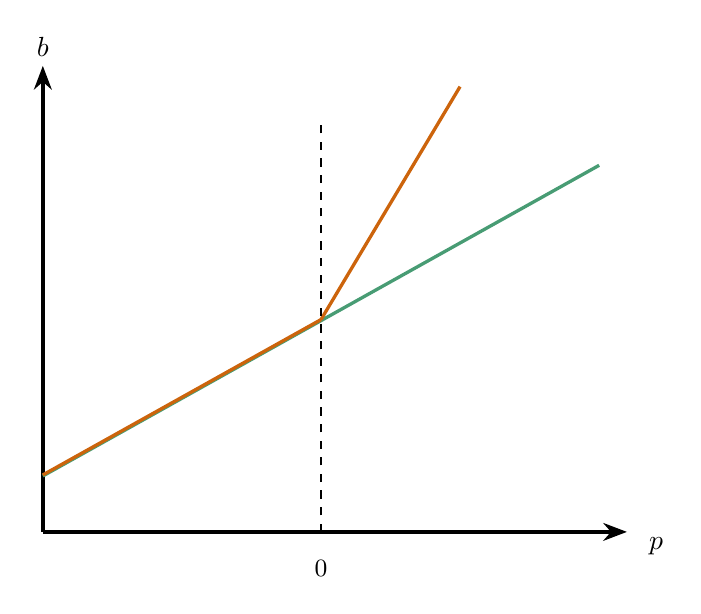
\begin{tikzpicture}
  \begin{axis}[
    width=9cm, height=7.5cm,
    axis lines=left,
    axis line style={-{Stealth[length=3mm]}, ultra thick},
    xmin=0, xmax=4.2, ymin=0, ymax=9,
    xtick=\empty, ytick=\empty, clip=false,
    xlabel={},
    xlabel style={at={(axis description cs:1.02,0)}, anchor=west},
    ylabel={},
  ]

    % Axis labels
    \node[anchor=south, rotate=0] at (axis description cs:0,1) {$b$};
    \node[anchor=south, rotate=0] at (axis description cs:1.05,-0.07) {$p$};

    % Black baseline line
    \addplot[very thick,col_before,domain=0:4] {1.08+1.5*x};

    % Orange shifted line (parallel, upward shift)
    \addplot[very thick,col_after,domain=0:2] {1.1+1.5*x};

    % Orange horizontal line
    \addplot[very thick,col_after,domain=2:3] {-4.9+4.5*x};

    %\node[col_after] at (axis cs:3,4.6) {$\Delta b_S$};

    \draw[dashed,black!60!black] (axis cs:2,0) -- (axis cs:2,8);

    % Arc to show angle
  %\draw[thick,col_after] (2.6,4) arc[start angle=0,end angle=22,radius=2];

    \node at (axis cs:{2},-0.7) {\small $0$};

  \end{axis}
\end{tikzpicture}
\bfootnote{\hyperlink{counterfactualDistribution}{\beamerbutton{Voltar}}}
\end{frame}

\begin{frame}[label=pureL]{Frequências da Reforma Pura em Nível para $t\geq 0$: Chegadas ao Limite}
\begin{itemize}
    \item Objetivo: obter as frequências \emph{puras em nível} $N^{L}_{p,t}$
    \item Número de postergadores vindos de $(p,s)$: $P_{p,s}\equiv N^{c}_{p,s}-N^{a}_{p,s}\quad\text{para }p<0$
    \item A2: os pontos se acumulam deterministicamente em $0.5$ por trimestre
    \item Para $p<0$, o postergador saindo de $(p,s)$ atinge o limite $p=0$ em $s-2p\equiv t$, de modo que as \emph{chegadas por postergação ao limite} no trimestre $t$ são:
    \[
        PA_{t} \equiv \sum_{p\in\{-6,-5.5,\dots,-0.5\}} P_{p,\;t+2p},
    \]
    \item Interpretação: $PA_{t}$ é o número de postergadores que pela primeira vez passam a poder requerer com $p=0$ (chegam ao limiar) no trimestre $t$
\end{itemize}
\end{frame}

\begin{frame}{Frequência da Reforma Pura em Nível}
    \begin{itemize}
        \item A2 implica que um requerimento em $(p,t)$ deve vir de chegadas em $t-2p$
        \begin{itemize}
            \item Ex.: os únicos postergadores que podem estar em $(p,t)=(1,4)$ são aqueles que chegaram em $t=2$ e então requereram 2 trimestres depois
        \end{itemize}
        \item O bunching por postergação em $(p,t)$ é dado pelas chegadas em $t-2p$ ($PA_{t-2p}$) vezes a probabilidade de requerer com $p$ dado que se chegou em $t-2p$ ($g_{p,t-2p}$):
    \[
        PB_{p,t}\equiv g_{p,t-2p}\cdot PA_{t-2p}
    \]
    \item Frequência pós-reforma pura em nível:
    \[
        N^{L}_{p,t}=
        \begin{cases}
            N^{a}_{p,t}, & p<0,\\[3pt]
            N^{c}_{p,t}+PB_{p,t}, & p\ge 0.
        \end{cases}
    \]
\end{itemize}
\end{frame}

\begin{frame}[label=gp_est]{Estimando $g_{p,t}$ a partir de Coortes de Chegada (Contagens)}
\begin{itemize}
    \item A3: o bunching só ocorre para \textcolor{red}{$p=0,1$}, o que corresponde a atrasos no requerimento de até \textcolor{red}{2} trimestres após atingir o limiar, justificado por:
        \begin{itemize}
            \item Nos primeiros períodos, a massa excedente pode ocorrer por antecipação sem bunching (que também só aparece até \textcolor{red}{$t=3$})
            % Suggesting that the less attentive ppl were inattentive for 3 quarters
            % If someone reaches p=0 and only responds 3 quarters later it will claim with 1.5 points
            \item Nos períodos posteriores $(t\geq \textcolor{red}{4})$, a massa excedente só é observada para \textcolor{red}{$p=0,1$}
            % When there is only actual bunching incentives, it is diffuse up to 4
        \end{itemize}
    \item A4 (Mistura Proporcional): condicional à chegada em $t$, antecipadores e postergadores requerem proporcionalmente em \textcolor{red}{$p=0,1$}. Note que
    \begin{itemize}
        \item Mesmo aqueles que chegam em $t=0$ podem requerer em $(p,t)=(1,2)$.
        \item Consideramos quem chega em $t\geq 0$, mas não os antecipadores já acima do limite no momento da reforma
    \end{itemize}
    \item Distribuição empírica de requerimento condicional às chegadas em $t>0$:
    \[
        \widehat{ g}_{p,t}\equiv
        \frac{\#\{i:\text{ arrived in } t\text{, and claimed with }p\}}
             {\#\{i:\text{ arrived in } t\text{, and claimed with }\textcolor{red}{p\in [0,1]}\}},
        \quad \textcolor{red}{p=0,1}
    \]
\end{itemize}
\bfootnote{\hyperlink{pureLStep}{\beamerbutton{Voltar}} }
\end{frame}

\begin{frame}[label=pureS]{Frequências Pós-Reforma Pura em Inclinação}
    \begin{itemize}
        \item Lembre que $EM_{p,t}\equiv N^a_{p,t}-N^c_{p,t},
        \quad p\geq 0,\; t\in\{0,1,2,3\}$, e defina $EM_{p,t}=0$ para $t>3$.
        % This is because the excess mass we are talking about is only for early quarters anticipation
        % The later quarters anticipation consist of individuals that had not arrived by t=0, would have claim at p>0 but anticpate to p=0. They would do the exact same thing under the pure-S reform.
        
        \item Defina a massa de antecipação que entra:
        \[
        A_{p,t}\equiv \frac12 EM_{p,t+1}+\frac12 EM_{p+1,t+1}.
        \]
        \item Então, para $p\geq 0$,
        \[
        N^S_{p,t}=N^c_{p,t}+A_{p,t}-PB_{p,t}.
        \]
         \item Como $EM_{p,t}=0$ para $t>3$, isso desliga automaticamente o ajuste de antecipação nos períodos posteriores, de modo que não é necessária uma terceira linha adicional.
    \end{itemize}
    \bfootnote{\hyperlink{pureSStep}{\beamerbutton{Voltar}} }
\end{frame}

\begin{frame}{Frequências Pós-Reforma Pura em Inclinação}
    \begin{itemize}
        \item A reforma pura em inclinação geraria todos os movimentos da reforma observada acima do limite, exceto a postergação:
    \end{itemize}
    \begin{align*}
            N^S_{p,t}&=\begin{cases} 
                N_{p,t}^c, & if\quad p<0 \\
                N_{p,t}^a - PB_{p,t}, & if\quad p\geq 0
            \end{cases}
        \end{align*}
    \begin{itemize}
        \item Como $PB_{p,t}=0$ fora de $p\in[0,4)$, essa subtração afeta apenas células nas quais pode surgir bunching por postergação
    \end{itemize}
\end{frame}

\begin{frame}[label=pureDetails]{Visão Geral do Cálculo das Reformas Puras}
\begin{itemize}
    \item As escolhas (por exemplo, requerimento, anos de contribuição, salário etc.) do indivíduo $i$ no trimestre $t$ são denotadas por $x_{it}$
    \begin{itemize}
        \item $x^a_{it}$: escolhas observadas após a reforma
        \item $x^c_{it}$: escolhas contrafactuais na ausência da reforma
        \item $x^L_{it}$: escolhas que teriam sido feitas sob a reforma pura em nível
    \end{itemize}
    \item Objetivo: construir 3 objetos análogos de benefícios sob cada reforma pura
    \begin{itemize}
        \item $b^{L}(x^a_{it})$: benefícios obtidos ao aplicar $b^{L}$ às escolhas observadas pós-reforma $x^a_{it}$
        \item $b^{L}(x^c_{it})$: benefícios mecânicos pagos sem respostas comportamentais
        \item $b^{L}(x^{L}_{it})$: benefícios sob a regra pura em nível usando apenas respostas comportamentais puras em nível
    \end{itemize}
    \item A mesma lógica vale para a reforma pura em inclinação ($b^{S}$)
\end{itemize}
\end{frame}

\begin{frame}{Passo 1: Computar os Gastos Observados $E^{a,L}_{p,t}$}
\begin{itemize}
    \item Aplicar a regra pura em nível $b^{L}$ às escolhas observadas pós-reforma $x^a_{it}$
    \item Aproximamos isso usando taxas de reposição (RR): ver o próximo slide
    
    \item {Computamos o gasto total em cada célula $(p,t)$ como:}
    \begin{align*}
        {E^{a,L}_{p,t} \equiv \sum_{i \in \{p|t\}} \sum_t^{T_i} \frac{b^L(x^a_{it})}{(1+r)^t}}
    \end{align*}
    
    \item {Note que isso corresponde a $N^a_{p,t}\,\bar b^L(x^a_{p,t})$ na notação anterior:}
    
    \item {$E^{a,L}_{p,t}$ é o valor presente do gasto total com aqueles que requerem com $p$ pontos no trimestre $t$ sob a regra pura em nível e escolhas observadas}
\end{itemize}
\end{frame}

\begin{frame}[label=menApprox]{Aproximações para $b^L(x_{it}^a)$ e $b^S(x_{it}^a)$}
    \begin{columns}
        \begin{column}{0.45\textwidth}
            \centering
            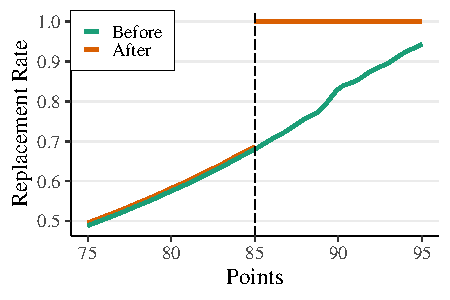
\includegraphics[width=\linewidth]{schedule_women_new.pdf}
        \end{column}
        \begin{column}{0.45\textwidth}
          \centering
          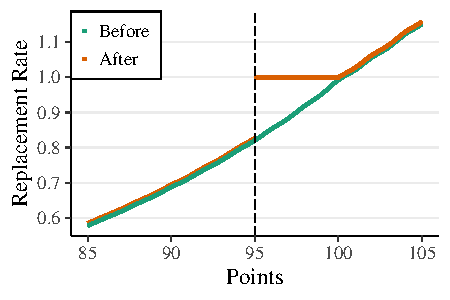
\includegraphics[width=\linewidth]{schedule_men_new.pdf}
        \end{column}
    \end{columns}
    {\small \begin{align*}
        RR(x_{it}^a) & = RR_{0} (x_{it}^a) + b_S(x_{it}^a)p(x_{it}^a) =\begin{cases}
            0.69+0.021p \text{ se $i$ é mulher} \\
            0.82+0.025p \text{ se $i$ é homem}
        \end{cases}
    \end{align*}}
    \begin{itemize}
        \item $b^L(x_{it}^a) = \begin{cases}
            b(x_{it}^a) & \text{se} \quad p(x_{it}^a)<0 \\
            b(x_{it}^a)\{1+[1-RR_{0}(x_{it}^a)]/RR(x_{it}^a)\} & \text{se} \quad p(x_{it}^a)\geq 0
        \end{cases}$
        \item $b^S(x_{it}^a) = \begin{cases}
            b(x_{it}^a) & \text{se} \quad p(x_{it}^a)<0 \\
            b(x_{it}^a)RR_{0}(x_{it}^a)/RR(x_{it}^a) & \text{se} \quad p(x_{it}^a)\geq 0
        \end{cases}$
    \end{itemize}
\end{frame}

\begin{frame}{Passo 2: Gasto Mecânico $E^{c,L}_{p,t}=\sum_{i \in \{p|t\}} \sum_t^{T_i} \frac{b^L(x^c_{it})}{(1+r)^t}$}
\begin{itemize}
    \item {Os gastos mecânicos são computados sob (i) $b^L$ e (ii) escolhas contrafactuais na ausência da reforma $x_{it}$}
    
    \item {Usamos um DD para recuperar o gasto contrafactual em cada célula}
\end{itemize}    
    \begin{align*}
        {E^{a,L}_{p,t}=\delta_{p}^{L}+\gamma_t^{L} +\sum_{k\neq -2}\beta_{\tilde{p},k}^{L} 1(p\in \tilde p)*1(t=k)+\varepsilon_{p,t}^{L}}
    \end{align*}
\begin{itemize}    
    \item {O mesmo DD de antes, mas usando $E^{a,L}_{p,t}$ (gastos) em vez de $\bar b^{L}(x^a_{p,t})$}
    
    \item {$\beta^{L}_{p,t}$ capta a seleção vinda de postergação e antecipação}
    
    \item {Para cada ponto normalizado $p$ e $t\geq 0$, obtemos $E^{c,L}_{p,t}
        \;=\;
        E^{a,L}_{p,t}
        \;-\;
        \hat \beta^{L}_{p,t}$:}
    \item {Alternativamente, podemos trabalhar com o DD original em que $\beta^{L}_{p,t}$ é um efeito sobre benefícios médios e então definir $E^{c,L}_{p,t}=N^{c}_{p,t}[\bar b^L(x^a_{p,t})-\hat \beta^{L}_{p,t}]$}
\end{itemize}
\end{frame}

\begin{frame}{Passo 2.1: Gasto Contrafactual $E^{c}_{p,t}=\sum_{i \in \{p|t\}} \sum_t^{T_i} \frac{b^c(x^c_{it})}{(1+r)^t}$}
\begin{itemize}
    \item {Os gastos contrafactuais são computados sob (i) $b^c$ e (ii) escolhas contrafactuais na ausência da reforma $x_{it}^c$}
    
    \item {Usamos um DD para recuperar o gasto contrafactual em cada célula}
\end{itemize}    
    \begin{align*}
        {E^{a,c}_{p,t}=\delta_{p}^{a,c}+\gamma_t^{a,c} +\sum_{k\neq -2}\beta_{\tilde{p},k}^{a,c} 1(p\in \tilde p)*1(t=k)+\varepsilon_{p,t}^{a,c}}
    \end{align*}
\begin{itemize}    
    \item {O mesmo DD de antes, mas usando $E^{a,c}_{p,t}=\sum_i \sum_t^{T_i} \frac{b^c(x^a_{it})}{(1+r)^t}$}
    
    \item {$\beta^{L}_{p,t}$ capta a seleção vinda de postergação e antecipação}
    
    \item {Para cada ponto normalizado $p$ e $t\geq 0$, obtemos $E^{c}_{p,t}
        \;=\;
        E^{a,c}_{p,t}
        \;-\;
        \hat \beta^{a,c}_{p,t}$:}
\end{itemize}
\end{frame}

\begin{frame}{Passo 3: Gastos Mecânicos sob a Reforma Pura em Nível}
\begin{itemize}
    \item Estes são os gastos mecânicos com benefícios mais altos, mas sem respostas comportamentais
    
    
    \item Agregamos os {gastos contrafactuais} ao longo dos pontos normalizados:
    \[
        \text{MECH}^{L}_t
        \;=\;
        \sum_{p} {E^{c,L}_{p,t}}
    \]
    
    \item Este é o valor presente do gasto total com benefícios sob a reforma $b^L$ na ausência de qualquer resposta comportamental para aqueles que requerem em $(p,t)$
\end{itemize}
\end{frame}

\begin{frame}{Passo 4: Gastos da Reforma Pura em Nível $E^{L}_{p,t}=\sum_{i \in \{p|t\}}\sum_i^{T_i} b^L(x^L_{it})$}
\begin{itemize}
    \item Como a reforma pura em nível gera {postergação}, mas não {antecipação}, só precisamos remover a seleção associada à segunda
    
    \item Como apenas a postergação afeta $p<0$:
    \[
        {
        E^{L}_{p,t} \;=\; E^{a,L}_{p,t}
        }\quad \text{para}\quad p<0,\ t\geq -1
    \]
    \item \textcolor{red}{Para $p\geq 0$ e $t=-1$, $E^{L}_{p,t}=E^{a,L}_{p,t}$ porque há postergação tanto na reforma observada quanto na reforma pura em nível:}
    \item Para $p\geq 0$ e $t\geq 0$, construímos os gastos combinando gastos contrafactuais com fluxos de postergação $E^{P,L}_{p,t}$:
    \[
        {
        E^{L}_{p,t}
        \;=\;
        E^{c,L}_{p,t}
        \;+\;
        E^{P,L}_{p,t}
        }
    \]
\end{itemize}
\end{frame}

\begin{frame}{Efeitos da Postergação: Exemplos}
    \begin{itemize}
        \item Ex1: os postergadores para $(p,t)=(1,6)$ vêm de $(-1,2)$ e $(-2,0)$, mas não podem vir de $(-3,-2)$, $(-4,-4)$, $(-5,-6)$ nem $(-6,-8)$
        \begin{itemize}
            \item Eles vêm de $(-x,t-2(x+1))$ para $x=1,2$
            \item {Todos esses grupos chegam ao limiar no trimestre $t-2p=4$, mas lembre que eles requerem com $1$ com probabilidade $g_{1,4}$}
        \end{itemize}
        
        \item Ex2: os postergadores para $(p,t)=(2,6)$ vêm de $(-1,0)$, mas não podem vir de $(-2,-2)$, $(-3,-4)$, $(-4,-6)$, $(-5,-8)$ nem $(-6,-10)$
        \begin{itemize}
            \item Eles vêm de $(-x,t-2(x+2))$ para $x=1$
            \item {Eles chegam ao limiar no trimestre $t-2p=2$, mas lembre que requerem com $2$ com probabilidade $g_{2,2}$}
        \end{itemize}
        
        \item {Construímos os gastos de postergação em $(p,t)$ a partir das perdas de gasto nas células de origem}
        \begin{align*}
        \text{Ex1:}\quad 
        {E^{P,L}_{1,6}}
        &{= g_{1,4}\Bigl[-E^{P,L}_{-1,2}-E^{P,L}_{-2,0}\Bigr]}
        \\
        \text{Ex2:}\quad 
        {E^{P,L}_{2,6}}
        &{= g_{2,2}\Bigl[-E^{P,L}_{-1,0}\Bigr]}
        \end{align*}
        \item {Onde $E^{P,L}_{p,t}=E^{a,L}_{p,t}-E^{c,L}_{p,t}$ para todo $p\in (-6,0)$ e $t\geq -1$}
    \end{itemize}
\end{frame}

\begin{frame}{Efeitos da Postergação: Caso Geral}
    \begin{itemize}
        \item Para ir de $-x$ até $p$, os indivíduos precisam de $2x$ períodos para chegar a zero e depois de $2p$ períodos para chegar a $p$
        
        \item Portanto, se eles foram de $-x$ para $p$ em $t$, precisam ter saído em $t-2(x+p)$
        
        \item Os postergadores para $(p,t)$ vêm de $(-x,t-2(x+p))$ para $x=1,..,\bar{x}_{p,t}$
        
        \item Onde $-\bar x_{p,t}$ é o ponto mais negativo de origem dos postergadores para $(p,t)$ associado ao trimestre do anúncio $t-2(\bar x_{p,t}+p)=-1$, se tal ponto for ao menos $-6$, isto é,
        \begin{align*}
            \bar x_{t,p}=\begin{cases}
                (t+1)/2-p & \text{se } (t+1)/2-p\leq 6 \\
                6 & \text{caso contrário.}
            \end{cases}
        \end{align*}
        \item {Lembre que todos esses grupos chegam ao limiar em $t-2p$ e requerem com $p$ com probabilidade $g_{p,t-2p}$}
        \item {Construímos os gastos totais de postergação em $(p,t)$ como a realocação das perdas de gasto vindas das células de origem}
        \begin{align*}
            E^{P,L}_{p,t}
            &=
            g_{p,t-2p}
            \sum_{x=1}^{\bar x_{t,p}}
            \left(
            -E^{P,L}_{-x,t-2(x+p)}
            \right)
            \quad \text{para } p \in [0,4)
        \end{align*}
    \end{itemize}
\end{frame}

\begin{frame}{Gastos Comportamentais e Contrafactuais da Reforma Pura em Nível}
    \begin{itemize}
        \item {Isso garante que recuperamos $E^{L}_{p,t}$ para todo $p$}
        
        \item Gastos comportamentais no trimestre $t$:
        \[
            {
            \text{BEHAV}^{L}_t
            \;=\;
            \sum_{p}
            E^{L}_{p,t}
            }
        \]
        
        \item {Combina o deslocamento comportamental puro em nível com os gastos realocados}
        
        \item Também podemos recuperar os gastos contrafactuais com benefícios como antes
        \begin{align*}
            {
            \text{CNTRF}_t
            =
            \sum_{p}
            E^{c}_{p,t}
            }\equiv \sum_{p}
            N^{c}_{p,t}\,
            \bar b(x_{p,t})
        \end{align*}
    \end{itemize}
\end{frame}



\begin{frame}{Resultados Finais}
    \begin{itemize}
        \item Podemos então calcular custos totais, efeitos mecânicos e efeitos de bem-estar para $b^L$ (como no slide 38) e obter os WMVPFs
        \begin{align*}
             TC^L_t &= \text{BEHAV}_t^{L} - \text{CNTRF}_t, \quad 
             ME^L_t = \text{MECH}_t^{L} - \text{CNTRF}_t \text{ and }\\ 
            WE^L_t &= ME^L_t \, \left(1-\gamma \frac{c_b - c_{pop}}{c_{pop}}-\right) \Rightarrow WMVPF_t^L = \frac{WE^L_t}{TC^L_t}
        \end{align*}
        
        \item Obter $\Delta b_L$ médio em $t=T$ (3T de 2018):
        \begin{align*}
            \Delta b_L = \frac{1}{N_T}\sum_{i}b(x^a_{iT})\frac{1-RR_{0}(x^a_{iT})}{RR(x^a_{iT})}
        \end{align*}
        
        \item Resultados: (i) densidades, (ii) gráfico de WE/FE/ME, (iii) $\Delta b_S$ e $\Delta b_L$, (iv) $TC_T$ e $TC_T^L$, e (v) WMVPFs para o último trimestre (3T de 2018)
    \end{itemize}
    \bfootnote{\hyperlink{disentangling}{\beamerbutton{Voltar}} }
\end{frame}

\begin{frame}{Passos Equivalentes para a Reforma Pura em Inclinação $b^{S}$ (1/2)}
\begin{enumerate}
    \item Computar ${b}^S(x^a_{it})$ e {os gastos em $E^{a,S}_{p,t} = \sum_{i \in \{p|t\}} b^S(x^a_{it})$}
    \item Estimar os efeitos de seleção com o seguinte DD
    \begin{align*}
        {E^{a,S}_{p,t}}=\delta_{p}^{S}+\gamma_t^{S} +\sum_{k\neq -2}\beta_{\tilde p,k}^{S} 1(p\in \tilde p)*1(t=k)+\varepsilon_{p,t}^{S}
    \end{align*}
    
    \item Corrigir o gasto em (1) usando seleção e obter o gasto mecânico total
    \[
    {
    E^{c,S}_{p,t}
    \;=\;
    E^{a,S}_{p,t}
    \;-\;
    \hat \beta^{S}_{p,t}
    \quad
    \text{ou usando o DD anterior }
    \quad
    E^{c,S}_{p,t}
    =
    N^{c}_{p,t}[\bar b^{S}(x_{p,t}^a)-\hat \beta^S_{p,t}]
    }
    \]
    
    \item Os gastos da reforma pura em inclinação corrigem (1) apenas pela seleção associada à postergação:
\end{enumerate}
{\tiny
    \[
    E^{P,S}_{p,t}
    =
    \begin{cases}
        E^{a,S}_{p,t}-E^{c,S}_{p,t} & \text{para } p<0 \\
        -g_{p,t-2p}
            \sum_{x=1}^{\bar x_{t,p}}
            {E^{P,S}_{-x,t-2(x+p)}} & \text{para } p\in [0,4) \\
        0 & \text{para } p\geq 4
    \end{cases} \Rightarrow
    E^{S}_{p,t}
    =
    \begin{cases}
        E^{c,S}_{p,t} & \text{para } p<0 \\
        E^{a,S}_{p,t}-E^{P,S}_{p,t} & \text{para } p\geq 0
    \end{cases}
    \]}
\end{frame}

\begin{frame}{Passos Equivalentes para a Reforma Pura em Inclinação $b^{S}$ (2/2)}
\begin{enumerate}
    \setcounter{enumi}{4}
    
    \item Agregar os {gastos} usando a densidade sob a reforma pura em inclinação
    \[
        \text{BEHAV}^{S}_t
        \;=\;
        \sum_{p}
        {E^{S}_{p,t}
        }
    \]
    
    \item Calcular custos totais, efeitos mecânicos e efeitos de bem-estar, e os WMVPFs:
    \begin{align*}
        TC^S_t &= \text{BEHAV}_t^{S} - \text{CNTRF}_t, \\
        ME^S_t &= \text{MECH}_t^{S} - \text{CNTRF}_t, \\
        WE^S_t &= ME^S_t \left(1-\gamma \frac{c_b - c_{pop}}{c_{pop}}\right), \\
        WMVPF_t^S &= \frac{WE^S_t}{TC^S_t}
    \end{align*}
    
    \item Obter $\Delta b_S$ médio usando a participação de homens e mulheres ($s_m/s_w$) como pesos
    \begin{align*}
        \Delta b_S = -(s_w*0.021+s_m*0.025)
    \end{align*}
    
    \item Gerar o gráfico dos insumos do WMVPF, $\Delta b_S$, $TC_T^S$ e $WMVPF_T^S$
\end{enumerate}
\bfootnote{\hyperlink{disentangling}{\beamerbutton{Voltar}} }
\end{frame}

\begin{frame}[label=optimalDetails]{Detalhes da Reforma Ótima Neutra em Orçamento}
    \begin{itemize}
        \item Qual reforma da regra aumenta mais o bem-estar?
        \begin{itemize}
            \item Local no sentido de que o governo só pode aumentar custos e receitas em um montante fixo igual a $C(b^c,b^a)$
        \end{itemize}
        \item Se o formulador de política precisa equilibrar seu orçamento com $b_S$ e $b_L$:
        \begin{itemize}
            \item Aumentar $b_S$ de modo que $dC/db_S * \Delta b_S^* = C(b^c,b^a)$
            \item Reduzir $b_L$ de modo que $dC/db_L * \Delta b_L^* = -C(b^c,b^a)$
        \end{itemize}
        \item Estimar $dC/db_S$ ($dC/db_L$) com $C(b,b_S)/\Delta b_S$ ($C(b,b_L)/\Delta b_L$)
        \item Vantagem de implementação:
        \begin{itemize}
            \item A \textbf{regra} previdenciária ótima depende de estatísticas suficientes sob a regra \textbf{ótima}
            \item A \textbf{reforma} previdenciária ótima depende de estatísticas suficientes sob a regra \textbf{observada}
        \end{itemize}
    \end{itemize}
    \bfootnote{\hyperlink{optimal}{\beamerbutton{Voltar}}}
\end{frame}

\begin{frame}[label=payroll]{Estimando o WNSBD}
    \begin{itemize}
        \item Obter os insumos para o WNSBD a partir da análise acima:
        {\footnotesize
        \begin{align*}
            WNSBD_p & = \frac{\sum_t\sum_xE(SMU_{it}|x)[b^p(x)-b(x)]-{WMVPF_T}(ME_p+BE_p)}{ME_p} \\
            & = \left(1-\gamma \frac{c_b - c_{pop}}{c_{pop}}-\right) - {WMVPF_T}\left(1+\frac{BE_p}{ME_p}\right),\quad \ \text{para} \ p=L,S
        \end{align*}}
        
        %\item Assumption: $SMU_{it}$ is constant ($\gamma \frac{c_b - c_{pop}}{c_{pop}}$) among beneficiaries
        
        \item Lobel (2025) encontra ${MVPF_T}\approx 1.64$, com incidência de 23\% sobre firmas (peso zero), 12\% sobre trabalhadores (consumo $c_w$) e 65\% sobre consumidores (consumo $c_p$), de modo que:
        \begin{align*}
            {WMVPF_T} = \left[.12\gamma \left(1-\gamma \frac{c_w - c_{pop}}{c_{pop}}-\right)+.65\right]1.64
        \end{align*}
    \end{itemize}
    \bfootnote{\hyperlink{expenditure}{\beamerbutton{Voltar}} }
\end{frame}

\end{document}
